%	-------------------------------------------------------------------------------
% 
%
%
%
%
%
%
%
%
%
%	-------------------------------------------------------------------------------
	\documentclass[12pt, a4paper, twoside]{book}
%	\documentclass[12pt, a4paper, twoside, openright]{book}
%	\documentclass[12pt, a4paper, oneside]{book}
%	\documentclass[12pt, a4paper, landscape, oneside]{book}


		% --------------------------------- 페이지 스타일 지정
		\usepackage{geometry}
%		\geometry{landscape=true	}
		\geometry{top 		=10em}
		\geometry{bottom		=10em}
		\geometry{left		=8em}
		\geometry{right		=8em}
		\geometry{headheight	=4em} % 머리말 설치 높이
		\geometry{headsep		=2em} % 머리말의 본문과의 띠우기 크기
		\geometry{footskip		=4em} % 꼬리말의 본문과의 띠우기 크기
% 		\geometry{showframe}
	
%		paperwidth 	= left + width + right (1)
%		paperheight 	= top + height + bottom (2)
%		width 		= textwidth (+ marginparsep + marginparwidth) (3)
%		height 		= textheight (+ headheight + headsep + footskip) (4)



		%	===================================================================
		%	package
		%	===================================================================
%			\usepackage[hangul]{kotex}				% 한글 사용
			\usepackage{kotex}						% 한글 사용
			\usepackage[unicode]{hyperref}			% 한글 하이퍼링크 사용
			\usepackage{amssymb,amsfonts,amsmath}	% 수학 수식 사용

			\usepackage{scrextend}					% 
		
		% ------------------------------ 개조식 문서 작성
			\usepackage{enumerate}			%
			\usepackage{enumitem}			%
			\usepackage{tabto}				%     tabto package
			\usepackage{tablists}			%	수학문제의 보기 등을 표현하는데 사용
										%	tabenum


		% ------------------------------ table 
			\usepackage{longtable}			%
			\usepackage{tabularx}			%
			\usepackage{tabu}				%

			\usepackage{setspace}			%
			\usepackage{booktabs}			% table
			\usepackage{color}				%
			\usepackage{multirow}			%
			\usepackage{boxedminipage}		% 미니 페이지
			\usepackage[pdftex]{graphicx}	% 그림 사용
			\usepackage[final]{pdfpages}	% pdf 사용
			\usepackage{framed}			% pdf 사용
			
			\usepackage{fix-cm}	
			\usepackage[english]{babel}
	
			\usepackage{tikz}%
			\usetikzlibrary{arrows,positioning,shapes}
			%\usetikzlibrary{positioning}
			



		% --------------------------------- 	page
			\usepackage{afterpage}			% 다음페이지가 나온면 어떻게 하라는 명령 정의 패키지
%			\usepackage{fullpage}			% 잘못 사용하면 다 흐트러짐 주의해서 사용
%			\usepackage{pdflscape}			% 
			\usepackage{lscape}			%	 


			\usepackage{blindtext}
	
		% --------------------------------- font 사용
			\usepackage{pifont}				%
			\usepackage{textcomp}
			\usepackage{gensymb}
			\usepackage{marvosym}






		% --------------------------------- 페이지 스타일 지정

		\usepackage[Sonny]		{fncychap}

			\makeatletter
			\ChNameVar	{\Large\bf}
			\ChNumVar		{\Huge\bf}
			\ChTitleVar	{\Large\bf}
			\ChRuleWidth	{0.5pt}
			\makeatother

%		\usepackage[Lenny]		{fncychap}
%		\usepackage[Glenn]		{fncychap}
%		\usepackage[Conny]		{fncychap}
%		\usepackage[Rejne]		{fncychap}
%		\usepackage[Bjarne]	{fncychap}
%		\usepackage[Bjornstrup]{fncychap}

		\usepackage{fancyhdr}
		\pagestyle{fancy}
		\fancyhead{} % clear all fields
		\fancyhead[LO]{\footnotesize \leftmark}
		\fancyhead[RE]{\footnotesize \leftmark}
		\fancyfoot{} % clear all fields
		\fancyfoot[LE,RO]{\large \thepage}
		%\fancyfoot[CO,CE]{\empty}
		\renewcommand{\headrulewidth}{1.0pt}
		\renewcommand{\footrulewidth}{0.4pt}
	
	
	
		% --------------------------------- 	section 스타일 지정
	
		\usepackage{titlesec}
		
		\titleformat*{\section}			{\large\bfseries}
		\titleformat*{\subsection}			{\normalsize\bfseries}
		\titleformat*{\subsubsection}		{\normalsize\bfseries}
		\titleformat*{\paragraph}			{\normalsize\bfseries}
		\titleformat*{\subparagraph}		{\normalsize\bfseries}
	
		\renewcommand{\thesection}			{\arabic{section}.}
		\renewcommand{\thesubsection}		{\thesection\arabic{subsection}.}
		\renewcommand{\thesubsubsection}	{\thesubsection\arabic{subsubsection}}
		
		\titlespacing*{\section} 			{0pt}{1.0em}{1.0em}
		\titlespacing*{\subsection}	  		{0ex}{1.0em}{1.0em}
		\titlespacing*{\subsubsection}		{0ex}{1.0em}{1.0em}
		\titlespacing*{\paragraph}			{0ex}{1.0em}{1.0em}
		\titlespacing*{\subparagraph}		{0ex}{1.0em}{1.0em}
	
	%	\titlespacing*{\section} 			{0pt}{0.0\baselineskip}{0.0\baselineskip}
	%	\titlespacing*{\subsection}	  		{0ex}{0.0\baselineskip}{0.0\baselineskip}
	%	\titlespacing*{\subsubsection}		{6ex}{0.0\baselineskip}{0.0\baselineskip}
	%	\titlespacing*{\paragraph}			{6pt}{0.0\baselineskip}{0.0\baselineskip}
	

		% --------------------------------- recommend		섹션별 페이지 상단 여백
		\newcommand{\SectionMargin}			{\newpage  \null \vskip 2cm}
		\newcommand{\SubSectionMargin}		{\newpage  \null \vskip 2cm}
		\newcommand{\SubSubSectionMargin}	{\newpage  \null \vskip 2cm}


	
		% --------------------------------- mini toc 설정
		\usepackage{minitoc}


%		\renewcommand*{\partheadstartvskip}{\null\vskip20pt}
%		\renewcommand*{\partheadendvskip}{\vskip2pt}
%		\renewcommand\beforeparttoc{}		
		
		
		% --------------------------------- 절의 목차
		\setcounter{parttocdepth}{1}
		\setlength{\ptcindent}{0pt}
		\renewcommand{\ptcfont}{\normalsize\rm}
		\renewcommand{\ptcCfont}{\normalsize\bf}
		\renewcommand{\ptcSfont}{\normalsize\rm}
		
		% --------------------------------- 장의 목차
		\setcounter{minitocdepth}{1}    	% Show until subsubsections in minitoc
		\setlength{\mtcindent}{12pt} 		% default 24pt




	
		% --------------------------------- 	문서 기본 사항 설정
		\setcounter{secnumdepth}{3} 		% 문단 번호 깊이
		\setcounter{tocdepth}{3} 			% 문단 번호 깊이
		\setlength{\parindent}{0cm} 		% 문서 들여 쓰기를 하지 않는다.
		

		% --------------------------------- 	찾아보기
		\usepackage{makeidx}
		\makeindex




		% --------------------------------- 	줄간격 설정
		\doublespace
%		\onehalfspace
%		\singlespace
		
		
% 	============================================================================== List global setting
%		\setlist{itemsep=1.0em}
	
% 	============================================================================== enumi setting

%		\renewcommand{\labelenumi}{\arabic{enumi}.} 
%		\renewcommand{\labelenumii}{\arabic{enumi}.\arabic{enumii}}
%		\renewcommand{\labelenumii}{(\arabic{enumii})}
%		\renewcommand{\labelenumiii}{\arabic{enumiii})}


	%	-------------------------------------------------------------------------------
	%		Vertical and Horizontal spacing
	%	-------------------------------------------------------------------------------
		\setlist[enumerate,1]	{ leftmargin=8.0em, rightmargin=0.0em, labelwidth=0.0em, labelsep=0.0em }
		\setlist[enumerate,2]	{ leftmargin=8.0em, rightmargin=0.0em, labelwidth=0.0em, labelsep=0.0em }
		\setlist[enumerate,3]	{ leftmargin=8.0em, rightmargin=0.0em, labelwidth=0.0em, labelsep=0.0em }
		\setlist[enumerate]	{ 	itemsep=0.0em, 
								leftmargin=6.0ex, 
								rightmargin=0.0em, 
								labelwidth=0.0em, 
								labelsep=4.0ex 
							}


	%	-------------------------------------------------------------------------------
	%		Label
	%	-------------------------------------------------------------------------------
%		\setlist[enumerate,1]{ label=\arabic*., ref=\arabic* }
%		\setlist[enumerate,1]{ label=\emph{\arabic*.}, ref=\emph{\arabic*} }
%		\setlist[enumerate,1]{ label=\textbf{\arabic*.}, ref=\textbf{\arabic*} }   	% 1.
%		\setlist[enumerate,1]{ label=\textbf{\arabic*)}, ref=\textbf{\arabic*)} }		% 1)
		\setlist[enumerate,1]{ label=\textbf{(\arabic*)}, ref=\textbf{(\arabic*)} }	% (1)
		\setlist[enumerate,2]{ label=\textbf{\arabic*)}, ref=\textbf{\arabic*)} }		% 1)
		\setlist[enumerate,3]{ label=\textbf{\arabic*.}, ref=\textbf{\arabic*.} }		% 1.

%		\setlist[enumerate,2]{ label=\emph{\alph*}),ref=\theenumi.\emph{\alph*} }
%		\setlist[enumerate,3]{ label=\roman*), ref=\theenumii.\roman* }



	

% ------------------------------------------------------------------------------
% Begin document (Content goes below)
% ------------------------------------------------------------------------------
	\begin{document}
	
		% ----------------------- 장 목차 생성 Initialization
			\noptcrule 	% part toc에서 줄이 침범하는 에러가 나서 줄긋기를 중지 시킴			
			\dominitoc 		
			\doparttoc
			\dopartlof
			\dopartlot
			



%	% 	--------------------------------------------------------- Title Page  Begin [ 약표제지 ]
%		\begin{titlepage}
%			\centering
%			\null
%			\vspace{2cm}
%			{지질 \huge\bfseries 암석} \par
%		\end{titlepage}
%		\newpage
%		\thispagestyle{empty}
	
	
	% 	--------------------------------------------------------- Title Page [ 표제지 ]
		\clearpage
		\begin{titlepage}
			\centering
			\null
			\vspace{2cm}
			{지질 \huge\bfseries 암석} \par
			\vspace{2cm}
			{\Large 김대희\par}
			\vfill
			% Bottom of the page
			{\large 2016.8.16 \par}
			\vspace{2cm}
		\end{titlepage}
		\newpage
		\thispagestyle{empty}



			\tableofcontents
			\listoffigures
			\listoftables





%% 	======================================================================================================================= part  암석 일반
	\addtocontents{toc}{\protect\newpage}	
	
	
		\part{암석 일반}
	

%% 	======================================================================================================================= part  암석 일반
	
	
	
% 	======================================================================================================================= chapter
	\clearpage
	\chapter{암석 일반}
	\minitoc				% Creating an actual minitoc



	\clearpage
%	----------------------------------------------------------------------------------------------------------------------- section
	\section{암석 일반}
	

				우리는 산과 들, 강과 계곡에서 갖가지 모양과 색깔의 암석을 만난다. 
				집 앞마당이나 마을 뒷동산, 공원에 있는 조경석만 보더라도 같은 모양이나 종류를 찾아보기 어렵다. 
				이 수많은 암석 중에서 다이아몬드(금강석)처럼 완벽한 구조 덕분에 영원히 변치 않는 경우도 있지만, 대개는 생성된 이후 변화와 소멸을 거듭하며 윤회의 삶을 산다.  \\
				

				예를 들어, 해변의 모래가 차곡차곡 쌓여 형성된 사암은 지하 깊은 곳에서 높은 압력과 열을 받아 규암으로 변성한다. 
				그 후 지반이 융기하여 지표에 노출되면 비, 바람 얼음 등에 의해 침식, 풍화되어 다시 모래가 된다. 
				이후 모래는 하천이나 강을 따라 바다로 흘러 들어가 다시 해변에 쌓인다. \\

				이와 같이 암석은 환경의 변화에 따라 형태가 달라지기 때문에 지구가 생겨난 이래 끊임없이 계속된 지질 변동의 역사를 고스란히 담고 있다. 
				그러므로 암석의 특성과 분포 지역을 제대로 알면, 그 지역의 과거 지질 환경과 지표 경관이 어떠했는지를 이해하는데 큰 도움이 된다.




% 	======================================================================================================================= chapter
	\clearpage
	\chapter{암석의 분류}
	\minitoc				% Creating an actual minitoc


	\clearpage
%	----------------------------------------------------------------------------------------------------------------------- section
	\section{	암석의 분류}
	
			마그마가 식어 \textbf{ 화성암 }이 되고 퇴적물이 굳어져 \textbf{ 퇴적암 }이 되고 
			기존 암석이 열과 압력의 영향을 받아 \textbf{ 변성암 }이 된다는 것은 예로부터 알려졌다.
			
			
			\setlength{\fboxsep}{10pt}
			\setlength{\fboxrule}{2pt}
			\begin{center}
			\fbox{화성암} \hfill
			\fbox{퇴적암} \hfill
			\fbox{변성암}
			\end{center}
			
			

			암석은 기원에 따라 크게 화성암(火成巖), 퇴적암(堆積巖), 변성암(變成巖)으로 나뉜다. 

	\clearpage
%	----------------------------------------------------------------------------------------------------------------------- section
	\section{화성암}

				화성암은 마그마, 즉 지구 내부의 물질이 녹아 만들어진 유체가 압력과 온도 조건이 바뀌면서 굳은 암석으로, 
				고결(固結) 당시의 깊이와 압력에 따라 \textbf{ 심성암 (深成巖) }과 \textbf{ 화산암 (火山巖) }으로 구분된다. \\
				
				심성암에는 마그마가 지각의 약한 곳을 뚫고 올라오다가 지하 깊은 곳에서 굳은 화강암, 섬록암(번쩍이는 녹색 암석), 반려암 등이 있다. 
				반면 지표 가까이서 굳거나 지표 위로 분출하여 형성된 유문암, 안산암(안데스산맥의 암), 조면암, 현무암 등은 화산암에 속한다.  \\
				
				화성암의 광물 구조는 마그마의 성분과 냉각 속도 등에 따라 차이가 나타난다. 
				
				보통 화산암은 세립질 광물로 이루어져 있지만, 심성암은 조립질 광물로 이루어져 있다.



	\clearpage
%	----------------------------------------------------------------------------------------------------------------------- section
	\section{퇴적암}

				퇴적암은 지표 위에 있던 암석이 공기나 물에 노출되어 침식과 풍화 작용으로 깎여나간 다음 
				물, 바람, 빙하에 의해 특정한 지역으로 옮겨져 쌓인 후 굳은 암석을 말한다. 
				이러한 풍화, 침식, 운반, 퇴적의 과정은 원을 그리며 끊임없이 반복한다.  
				
				\paragraph{쇄설성퇴적암, 화학적 퇴적암} 
				이 가운데 진흙이 쌓여 만들어지는 이암과 모래가 쌓여 만들어지는 사암, 그리고 모래, 자갈, 진흙 등이 섞이고 쌓여 만들어지는 역암은 
				\textbf{ 쇄설성 퇴적암 }에 속하고, 
				산호, 조개 껍데기 등의 화학적 침전물이 쌓여 만들어지는 석회암은 \textbf{ 화학적 퇴적암 }에 속한다. 
				\paragraph{층리} 
				퇴적암에는 평행한 줄무늬인 층리가 나타나는데, 이것은 퇴적물이 오랜 세월 여러 겹으로 쌓인 결과로 쉽게 알아볼 수 있다. 
				\paragraph{화석} 
				또한 퇴적암에는 생물의 유해나 흔적이 화석으로 남아 있는 경우가 많은데, 이를 통해 퇴적 당시의 자연 환경을 추측할 수 있다.



	\clearpage
%	----------------------------------------------------------------------------------------------------------------------- section
	\section{변성암}

				\paragraph{변성암} 
				변성암은 지표 부근의 화성암이나 퇴적암이 지하 깊은 곳으로 이동한 다음, 높은 열과 압력을 받아 본래의 암석과 성질이나 조직이 전혀 다른 새로운 암석으로 변한 것을 말한다. 
				예를 들면, 규암은 사암이, 대리암은 석회암이 변성 된 것이다.  \\

				\paragraph{변성암의 구분} 
				변성암은 변성 요인에 따라 \textbf{ 접촉 변성암 }과 \textbf{ 광역 변성암 }으로 구분되며, 열과 압력의 정도에 따라서도 다양한 암석이 나타난다.  \\
 
				진흙이 쌓여 이루어진 이암의 경우, 온도와 압력이 높아짐에 따라 점판암 $\rightarrow$ 천매암 $\rightarrow$ 편암 $\rightarrow$ 편마암 순으로 변한다. \\

				변성암은 화성암이나 퇴적암보다 한 번 더 지질 역사를 경험했기 때문에 상대적으로 복잡한 암석이라 할 수 있다. 
				높은 열과 엄청난 압력을 받으면 암석을 구성하는 광물의 일부가 녹아버리기도 하고 새로운 광물이 생겨나기도 하며, 본래 있던 광물들이 재배치되는 과정에서 방향성을 띠거나 일렬로 늘어서기도 한다. 

				\paragraph{편리, 엽리} 
				변성암에 발달한 줄무늬를 편리 또는 엽리라고 하는데, 일반인들이 퇴적암에 발달한 층리와 변성암에 나타나는 엽리를 구분하는 것은 쉽지 않다.
	
	


% 	======================================================================================================================= chapter
	\clearpage
	\chapter{광물과 암석이 형성되는 과정}
	\minitoc				% Creating an actual minitoc



	\clearpage
%	----------------------------------------------------------------------------------------------------------------------- section
	\section{광물과 암석이 형성되는 과정}
	


			\paragraph{화성암 암석 성인론}
			
			마그마가 식어 화성암이 되고 퇴적물이 굳어져 퇴적암이 되고 기존 암석이 열과 압력의 영향을 받아 변성암이 된다는 것은 예로부터 알려졌다. 
			그러나 20세기 들어 더욱 자세히 연구되어 화성암을 만드는 광물들이 결정되는 순서가 밝혀져 화성암의 형성 과정이 제대로 알려지기 시작했다.  \\
			
			즉 1928년에는 캐나다에서 태어나 미국에서 활동한 실험과 이론에 밝은 암석학자 노만 L. 보웬(1887~1956)이 화성암의 성인에 반응 원리를 도입한 새로운 체계의 화성암 암석 성인론을 수립했다.  \\

			예를 들면, 유색 광물은 감람석, 휘석류, 각섬석, 흑운모 같은 \textbf{ 철 }이나 \textbf{ 마그네슘 }이 많은 광물들이 압력이 높고 온도가 높은 환경에서 먼저 만들어진다. 
			감람석도 처음에는 마그네슘이 많으나 시간이 가면서 적어지는 대신 철이 많아지고 휘석류도 알칼리 성분이 많아진다. 
			또 시간이 가면서 온도가 낮아지고 압력이 떨어지면서 백운모에 이어 석영 같은 무색광물들이 만들어진다. 이 과정은 불연속이 



% 	======================================================================================================================= chapter
	\clearpage
	\chapter{암석 나이의 측정}
	\minitoc				% Creating an actual minitoc


	\clearpage
%	----------------------------------------------------------------------------------------------------------------------- section
	\section{암석 나이의 측정}
	



1. 		암석 나이의 측정

page 21













%% 	======================================================================================================================= part  화성암
	\addtocontents{toc}{\protect\newpage}	
	
	
		\part{화성암}
	



% 	======================================================================================================================= chapter
	\clearpage
	\chapter{화성암 일반}
	\minitoc				% Creating an actual minitoc
	

	\clearpage
%	----------------------------------------------------------------------------------------------------------------------- section
	\section{화성암}



		지질은 총 세가지로 분류됩니다.(변성암,화성암,퇴적암)
		그중 화성암은 또 세가지로 분류되죠.(화산암,반심성암,심성암)

		\paragraph{마그마의 위치}
		마그마(땅속에있으면 마그마 땅위에 있으면 용암이라고 부릅니다)가 지표근처에 있는 화성암을 화산암이라고 부르구요, 
		땅속 깊이 있을때를 심성암이라고 부릅니다.(반심성암은 중간정도라고 이해하시면 됩니다.)

		\paragraph{화산암에서의 이산화 규소 량}
		근데 여기서 화산암을 이산화규소(SiO2)의 함량으로 세가지로 분류하는데요
		이산화 규소의 함량이 적은 순서대로 현무암질-안산암질-유문암질 이렇게 분류합니다. 

		이산화규소의 함량이 높을수록 용암의 점성이 높고 유동성이 적으며, 온도가 낮고, 화산 폭팔 시에 큰 화산폭발을 만들어내게 되고, 
		화산가스의 양을 많이 가지고 있고, 경사가 급한 화산을 이룹니다(경사가 완만한순서대로 순상화산-성층화산-종상화산)

		
		\paragraph{이산화 규소의 량이 많으면}

			\begin{itemize}[	topsep=0.0em, itemsep=-0.5em, leftmargin=4em, labelsep=3em ] 
			\item	용암의 점성이 높고
			\item	유동성이 적으며
			\item	온도가 낮고
			\item	화산 폭팔 시에 큰 화산폭발을 만들어내게 되고, 
			\item	화산가스의 양을 많이 가지고 있다.
			\item	경사가 급한 화산을 이룹다.
			\end{itemize}	
		

		\paragraph{심성암에서의 이산화 규소 량}
		그리고 이번엔 심성암을 보게되면 심성암은 구성되고있는 광물의 양에 따라 분류하면
		반려암,섬록암,화강암(이산화 규소의 함량이 적은순서대로) 등 이있습니다.

		질문을 설명드리자면 화산암의 이산화규소 함량의 따른 분류가 현무암질$<$안삼암질$<$유문암질 이구요,
		심성암을 비교를 위하여 이산화규소 함량에따라 나눠본 분류는 반려암질$<$섬록암질$<$화강암질 입니다

		그러니까 당연히 현무암질과 화강암질이섞이면 중간쯤인 안산암질이 되겠고,
		현무암질과 유문암질이 섞인다면 역시 중간쯤인 안산암질이 되겠죠...






		\paragraph{용암}
			용암(熔岩, 이탈리아어: lava)은 화산이 분출하는 동안 밖으로 나온 암석의 용융체이다. 
			처음 화산의 화구에서 빠져나올 때 용암의 온도는 700 °C에서 1,200 °C이다. 
			용암은 물에 비해 점성이 약 100,000배로 매우 점성질이지만, 요변성과 전단력으로 얇아지는 특성을 지녔기 때문에 냉각을 거쳐 굳을 때까지 매우 먼 거리를 이동하며 흐를 수 있다. 
			용암류(Lava flow)는 용암이 유출되어 나오는 것으로 비폭발적인 유출성 분출 중 생긴다. 
			움직임이 멈추면 용암은 굳어 현무암이 된다. 
			용암류를 줄여서 흔히 용암이라 부르기도 한다. 
			폭발적인 분출은 용암류와는 다른 화산재와 다른 파편들이 혼합된 테프라(tephra)를 만든다. 
			'lava'라는 말은 이탈리아어에서 나왔는데, '떨어지고', '미끄러지는' 의미의 라틴어 'labes'에서 유래되었을 것으로 본다. 
			분출된 마그마(지표 아래의 암석이 용융된 것)와 연관하여 처음 사용한 것은 프란시스코 세라오(Francesco Serao)가 1737년 5월 14일에서 6월 4일 동안에 베수비우스에서 분출한 것에 쓴 글에 나온다. 
			Serao는 호우에 뒤이어 화산의 옆구리 아래로 물과 진흙이 흘러가는 것을 "불붙는 용암의 흐름(a flow of fiery lava)"으로 기술하였다.

		\paragraph{용암}
			화산에서 뿜어저나온다. 
			화산 안에서 가장 약한 부분을 찾으면 뿜어져나온다. 
			화산의 안에 있으면 마그마지만, 화산 밖으로 뿜어져 나오는 순간 용암이 된다.

		\paragraph{용암과 마그마}
			용암은 화산 밖에 있고, 마그마는 화산 안에 있다. 
			화산 안에 있는 마그마는 가스를 가지고 있지만, 화산 안에서 나가는 순간, 가스가 증발해 용암이 되는 것이다. 
			그래서 용암과 마그마가 다르다.

		\paragraph{아아 용암}
			현무암질 용암의 표면 형상에 대하여 붙인 명칭이다. 
			아아는 하와이의 토착어(土着語)이며, 하와이의 화산에서 표면이 반들반들한 파호이호이 용암(Pahoehoe lava)에 대응하여 이 이름을 붙였다. 
			용암류의 두께는 보통 몇 m에서 몇십 m에 이른다.



	

	\clearpage
%	----------------------------------------------------------------------------------------------------------------------- section
	\section{마그마}




	\subsection{마그마}

				\begin{itemize}[topsep=0.0em, parsep=0.0em, itemsep=0em, leftmargin=12.0em, labelwidth=3em, labelsep=3em] 
				\item	염기성 현무암질 마그마
				\item	산성 화강암질 마그마

				\item	밝은 색의 산성 암맥
				\item	어두운 색의 염기성 암맥
				\end{itemize}






	\clearpage  \null
	\subsection{염기성, 중성, 산성 마그마}

				또한 마그마는 규소의 함량(함량)에 따라 어두운 색에서 밝은 색까지 다양하게 존재하는데, 규소의 함량이 많아지는 순서로 염기성(현무암질 , SiO2 함량 52\% 이하), 중성(안산암질), 산성(유문암질 SiO2 함량 66\% 이상) 마그마로 분류하기도 한다.  \\

		%		\tabulinesep=0.6ex
				\begin{tabu} to 1.0\textwidth { X[c, 2.0] X[c, 2.0] X[c, 2.0] }
				\tabucline[0.2ex]{-}		
				염기성\newline(규소함량이 적다) 	&중성		&산성\newline(규소함량이 많다)\\
				현무암질				&안산암질		&유문암질\\
				\tabucline[0.1ex]{-}		
				\end{tabu}  \null \\ \vskip 2em
	

		%		\tabulinesep=0.6ex
				\begin{tabu} to 1.0\textwidth { X[c, 2.0] X[c, 2.0] }
				\tabucline[0.2ex]{-}		
				염기성 마그마			&산성 마그마 \\
				\tabucline[0.2ex]{-}		
				깊은 곳에서 생성 		&온도가 높고 유동성이 크다 \\
				규소 함량이 작다			&얕은 곳에서 생성 \\
				온도가 낮고 유동성이 작다	&규소 함량이 많다 \\
				\tabucline[0.1ex]{-}		
				\end{tabu}  \\
	


				보통 염기성 마그마가 상대적으로 온도가 높고 유동성 큰 반면, 산성마그마는 온도가 낮고 유동성이 작다. \\
				
				대륙이나 해양 지각보다 더 깊은 맨틀이라는 곳에서 처음 만들어지는 마그마는 아마도 규소의 함량이 적은 염기성 마그마일 것으로 생각되며, 제주도의 현무암은 바로 이러한 염기성 마그마가 분출하여 굳은 것이다
				



				\paragraph{내 생각 정리}
				
				대륙 깊은 곳 맨틀에서 처음 만들어지는 마그마는 지각의 대부분을 차지하는 규소의 함량은 작을 것이다. 
				맨틀은 무거운 철분이 대부분을 차지하므로 따라서 지하 깊은 곳에 생성되어 온도가 높고 온도가 높으므로 유동성 또한 크다. 
				철과 마그네슘 성분 등을 많이 함유 하므로 색깔로 어두운 색을 띈다. 
				하지만 얕은 곳에서 생성되는 마그마는 지각의 대부분을 차지하는 규소를 충분히 함유하므로 상대적으로 낮은 온도에서 생성 되며 온도가 낮으므로 점성도 작다, 하지만 규소의 함량이 크므로 밝은 색을 띈다. 화강암이 된다.
				

	\subsection{마그마의 성질 변동}

				마그마는 냉각되면서 굳어질 때, 처음 만들어진 성분을 그대로 유지하지 못하는 경우가 많다..  \\
				
				예를 들어 염기성 마그마의 경우, 처음에 철과 마그네슘을 함유한 광물들이 먼저 결정으로 정출되는데, 이러한 광물의 순차적인 정출은 마그마 성분에 있어서 철, 마그네슘, 칼슘 성분이 줄어들고 규소, 나트륨, 칼륨의 함량을 증가시키는 결과를 가져온다. 
				결국 마그마의 조성은 염기성에서 산성으로 변화 될 수 있다. \\
				
				또한 마그마가 상승하면서 주변 암석을 포획하여 내부에 포함하는 경우, 이러한 주변 지가물질의 혼합 정도에 따라 마그마의 성분은 변화 될 것이다. 
				이럴 경우 원래의 마그마 성분을 알아낸다는 것은 매우 어려운 일이다. 
				실제로 충북 보은지역에 분포하는 중생대 쥐라기 화강암에 대한 결정작용과 동시성 혼합작용의 이론적 모델에 따른 좌용주(1996)의 연구에 의하면 
				이 화강암을 만든 화강암질 마그마는 이 지역을 관입하기 이전에 마그마 전체 질량의 약 10\% 내외의 퇴적 기원의 지각물질과 혼합된 것으로 계산되었다. 
				보통 염기성 현무암질 마그마에 규소 성분이 많은 지각물질이 혼합된다면 이 마그마는 규소의 함량이 많아지는 중성 내지 산성 마그마로 변화된다.  \\
				
				결국 화성암을 만든 마그마는 맨틀 기원의 마그마, 광물 정출과 분리에 따라 형성되는 여러 가지 조성의 마그마, 지각 물질의 첨가에 따라 조성이 변화된 마그마, 지각 물질이 녹아 만들어진 마그마 등 여러 가지 기원을 생각할 수 있다.



	\clearpage
%	----------------------------------------------------------------------------------------------------------------------- section
	\section{마그마의 분류}




	\subsection{마그마의 분류}


				\begin{itemize}[topsep=0.0em, parsep=0.0em, itemsep=0em, leftmargin=12.0em, labelwidth=3em, labelsep=3em] 
				\item	염기성 현무암질 마그마
				\item	산성 화강암질 마그마
				\end{itemize}




	\subsection{마그마의 분류}

			마그마는 $SiO_2$ 함량으로 그 조성범위를 특정 지울 수 있는데, 일반적으로 sio₂함량이 50\%내외인 현무암질(반려암질) 마그마 , 60\% 내외인 안산암질(섬록암질) 마그마, 70\% 내외인 유문암질(화강암질) 마그마로 구분된다. 

				\begin{itemize}[topsep=0.0em, parsep=0.0em, itemsep=0em, leftmargin=12.0em, labelwidth=3em, labelsep=3em] 
				\item	현무암질 마그마
				\item	안산암질 마그마
				\item	유문암질 마그마
				\end{itemize}



	\clearpage  \null
	\subsection{염기성, 중성, 산성 마그마}

				또한 마그마는 규소의 함량(함량)에 따라 어두운 색에서 밝은 색까지 다양하게 존재하는데, 규소의 함량이 많아지는 순서로 염기성(현무암질 , SiO2 함량 52\% 이하), 중성(안산암질), 산성(유문암질 SiO2 함량 66\% 이상) 마그마로 분류하기도 한다. 
				
		%		\tabulinesep=0.6ex
				\begin{tabu} to 1.0\textwidth { X[c, 2.0] X[c, 2.0] X[c, 2.0] }
				\tabucline[0.2ex]{-}		
				염기성\newline(규소함량이 적다) 	&중성		&산성\newline(규소함량이 많다)\\
				현무암질				&안산암질		&유문암질\\
				\tabucline[0.1ex]{-}		
				\end{tabu}  \null \\ \vskip 2em
	

		%		\tabulinesep=0.6ex
				\begin{tabu} to 1.0\textwidth { X[c, 2.0] X[c, 2.0] }
				\tabucline[0.2ex]{-}		
				염기성 마그마			&산성 마그마 \\
				\tabucline[0.2ex]{-}		
				깊은 곳에서 생성 		&온도가 높고 유동성이 크다 \\
				규소 함량이 작다			&얕은 곳에서 생성 \\
				온도가 낮고 유동성이 작다	&규소 함량이 많다 \\
				\tabucline[0.1ex]{-}		
				\end{tabu}  \\
	
				
	
				보통 염기성 마그마가 상대적으로 온도가 높고 유동성 큰 반면, 산성마그마는 온도가 낮고 유동성이 작다. 
				
				대륙이나 해양 지각보다 더 깊은 맨틀이라는 곳에서 처음 만들어지는 마그마는 아마도 규소의 함량이 적은 염기성 마그마일 것으로 생각되며, 제주도의 현무암은 바로 이러한 염기성 마그마가 분출하여 굳은 것이다
				
				\paragraph{내 생각 정리}
				
				대륙 깊은 곳 맨틀에서 처음 만들어지는 마그마는 지각의 대부분을 차지하는 규소의 함량은 작을 것이다. 
				맨틀은 무거운 철분이 대부분을  차지하므로 따라서 지하 깊은 곳에 생성되어 온도가 높고 온도가 높으므로 유동성 또한 크다. 
				철과 마그네슘 성분 등을 많이 함유 하므로 색깔로 어두운 색을 띈다. 
				하지만 얕은 곳에서 생성되는 마그마는 지각의 대부분을 차지하는 규소를 충분히 함유하므로 상대적으로 낮은 온도에서 생성 되며 온도가 낮으므로 점성도 작다, 하지만 규소의 함량이 크므로 밝은 색을 띈다. 화강암이 된다.





	\clearpage
%	----------------------------------------------------------------------------------------------------------------------- section
	\section{산성 마그마}





	\subsection{산성 마그마}


	\subsection{화강암질 마그마 [ granitic magma ] }

				화강암질 마그마는 무수환경 시 일정 압력이 있는 대륙판의 충돌 지역에서 생성된다. SiO2 함량이 약 66\% 이상으로 용융점이 낮고, 점성이 크며, 유동성이 작아 경사가 급한 종상화산을 만든다. \\
				
				지하 깊은 곳은 고온·고압이지만 온도와 압력이 균형을 이루고 있어서 지각이나 맨틀은 고체 상태를 유지하고 있는 것으로 알려져 있다. 그러나 온도와 압력이 변하면 용융이 일어나게 된다.  \\
				
				마그마의 생성 장소는 대체로 맨틀 및 지각 하부이며, 고체의 맨틀과 지각이 액체의 마그마가 되기 위해서는 그 온도를 일시적이라도 상부 액상선(liquidus) 이상으로 올려야 한다. 
				즉 용융 곡선에 접해야 한다. 
				그러기 위해서는 다음과 같은 몇 가지의 조건들을 생각할 수 있다.
				
				\begin{itemize}[topsep=0.0em, parsep=0.0em, itemsep=0em, leftmargin=6.0em, labelwidth=3em, labelsep=3em] 
				\item	[①] 	압력의 강하에 따른 용융점의 강하
				\item	[②] 	압력이 일정할 때의 온도의 상승
				\item	[③] 	기계적 에너지가 열적 에너지로 전환
				\item	[④]	온도, 압력이 일정할 때 $H_2O$ 등의 첨가로 고상선(solidus)의 강하 등이다.
				\end{itemize}
				
				
				①의 경우에는 어떤 이유로 지각 운동이 일어나면 이제까지 걸려있던 압력이 급강하하면서 용융점이 내려가는 경우이다. 
				
				②의 경우는 맨틀물질의 대류로 인하여 고온의 물질이 상승할 때 압력의 감소로 일어나며 주로 해령에서 일어난다. 
				
				③의 경우는 두 개의 판(plate)이 부딪칠 때 밀도차 때문에 하부로 스며들어가는 하나의 판이 생길 경우 등이다. 
				
				④의 경우는 실험적인 결과로 화강암은 H2O를 과잉으로 가해주면 10Kbar일 때 용융이 시작되는 무수(無水) 조건일 때보다 600°C 까지 저하되는 사실이 밝혀졌다. \\
				
				화강암질 마그마는 무수환경시 일정 압력이 있는 대륙판의 충돌 지역에서 생성된다. 위 그림에서 대륙지각의 지하 증온율과 H2O로 포화된 고체의 용융선(B)이 만나는 조건에서 형성된다. \\
				
				어떤 주어진 온도와 압력에서 암체는 일부분만 용해되고 용융물질의 성분은 원래의 암석과 전혀 달라질 수 있는데, 이 작용을 부분용융이라고 한다.  \\
				
				화강암질 마그마는 섭입대에서, 즉 두 판이 충돌하여 온도와 압력이 높은 곳에서 부분용융에 의해 생성된다. \\
				
				마그마는 sio₂함량으로 그 조성범위를 특정 지울 수 있는데, 일반적으로 sio₂함량이 50\%내외인 현무암질(반려암질) 마그마 , 60\% 내외인 안산암질(섬록암질) 마그마, 70\% 내외인 유문암질(화강암질) 마그마로 구분된다.  \\
				
				세 종류의 마그마의 산출 정도는 균등하지는 않아서 화산분출시 마그마의 80\% 정도가 현무암질 마그마이며, 안산암질 마그마와 유문암질 마그마는 각각 10\% 내외이다.  \\
				
				화강암질 마그마는 마그마의 분화 과정에서도 생성되는데 결정 분화작용 말기에 저온에서 형성되며, 주요 광물은 석영, 정장석, Ca사장석, 각섬석, 흑운모 등으로 구성되어 있다. 
				화강암질 마그마는 산성의 마그마로 용융점이 낮고, 점성이 크며, 유동성이 작아 주로 경사가 급한 화산체를 만든다.   \\
				
				[ 네이버 지식백과 ] 화강암질 마그마 [granitic magma] (두산백과)



	\clearpage
%	----------------------------------------------------------------------------------------------------------------------- section
	\section{염기성 마그마}
	





	\subsection{염기성 마그마   basic magma, 鹽基性─  }

			규산을 함유한 염기성암을 생성하는 마그마이다. 

			이 마그마에 의해 생성되는 암석은 규산(硅酸)을 45∼52\% 함유한다(규산의 함량이 작다). 
			염기성암으로서는, 심성암인 반려암, 반심성암인 반려분암, 화산암인 현무암이 있다. 
			
			[네이버 지식백과] 염기성마그마 [basic magma, 鹽基性─] (두산백과)
			



	\clearpage  \null
	\paragraph{한화케미칼 Hanwha Chemical/재미있는 화학 이야기 염기성 물질, 씁쓸하지만 없어서는 안 될 이 녀석을 파헤쳐보자! 2012.10.19 11:25 }

 

 
 
				좀처럼 떨어지지 않는 감기만큼 독한 것, 바로 감기약이죠~
				     너무 써서 얼굴마저 찌푸리게 되는 감기약, 왜 이렇게 맛이 없는 걸까요?  \\
				 
				하늘이 높고 말이 살이 찐다는 천고마비의 계절, 가을이 왔습니다. 
				독서를 즐기는 분들이 많아지기도 하고 야외활동을 하기 좋은 날씨 때문에 주말에 가족이나 친구분들과 함께 등산을 가시는 분들도 많아졌죠. 
				저 역시, 이번 주말 약속을 잡고 일주일을 손꼽아 기다리고 있었는데, 왠걸! 막상 주말이 되니 몸도 무거워지고 콧물은 훌쩍훌쩍 거리고 몸은 으슬으슬 거리기 시작합니다.ㅠㅠ 이런 ~ ~  슬프게도 감기에 걸리고 말았네요   \\
				 
				가을은 일교차가 클 때 감기에 걸리기 쉽다는 것은 일반적으로 많이 알려진 사실입니다. 
				감기에 걸리기 쉬운 환절기에는 감기에 걸리지 않도록조심해야 하는데요, 이렇게 한번 감기가 걸리면 먹기는 싫지만 감기약이라도 먹어서 빨리 낳으려고 합니다. 
				감기약은 아무 맛도 없거나 약간은 달달한 맛도 있지만 쓴 맛을 갖는 약들이 많이 있습니다. 
				그래서 쓴 맛이 싫어서 약을 거부하거나 혹은 약을 복용하여도 그 뒤에 오는 쓴맛을 제거하고 싶어서 사탕이나 초콜릿과 같은 단 맛을 내는 음식을 먹기도 합니다. \\
				 
				그런데 병을 치료해주는 감기약은 왜 이렇게 쓸까요? \\
				 
				감기약 속에 사용되는 성분들은 여러가지가 있지만 쓴 맛을 내는 물질에는 약한 염기성 물질이 들어 있습니다. 
				감기약 뿐 만 아니라 제산제와 같은 위산을 중화시키는 약의 경우에도 염기성 물질이 함유되어 쓴 맛을 느끼게 됩니다.
				이렇게 쓴 맛을 느끼게 해주는 염기성 물질! 씁쓸한 맛 때문에 싫지만 그래도 우리 생활 속에서 많이 사용되고 있는데요, 오늘은 주변에 조용히 숨어있는 염기성 물질에 대해서 알아보겠습니다. \\
				 
				씁쓸한 맛을 느끼게 하는 염기성 물질, 과연 무엇 때문에 염기성이라는 단어를 붙일까요? 염기라는 단어를 붙일 수 있는 물질들은 일반적으로 세가지 정의에 의해서 정해지게 됩니다.
				 
				\paragraph{첫 번째로} 물에 녹아서 수산화 이온을 내놓는 물질을 일반적으로 염기라고 합니다. 가장 대표적인 것이 수산화 나트륨(Sodium hydroxide, NaOH)입니다.
					 수산화 나트륨은 물에 녹아서 나트륨이온과 수산화 이온으로 나누어 지면서 염기성을 띄게 됩니다. 강한 염기로 알려져 있어서 강한 산성 물질을 중화 시킬 때 사용되고 있습니다.
				\paragraph{두 번째로는} 산성 물질에서 나오는 수소이온을 가져갈 수 있는 물질을 염기라고 합니다. 
						이러한 정의에 가장 잘 맞는 물질이 암모니아(Ammonia, NH3)입니다. 
						암모니아를 가장 잘 느낄 수 있는 곳이 삭힌 홍어인데요, 홍어 특유의 냄새와 맛은 바로 이 암모니아 때문인데요, 암모니아는 수산화이온을 가지고 있지 않지만, 약한 염기성을 가지고 있습니다. 
						이것은 암모니아 분자 속에 있는 질소 원자가 수소이온을 가져갈 수 있어서 산성물질과 만나면 암모니아는 암모늄(Ammonium, NH4+)이라는 물질로 바뀌게 됩니다.
				 
				\paragraph{마지막으로} 전자쌍을 줄 수 있는 경우 염기라는 물질로 정의하게 됩니다. 이 정의는 어렵게 느낄 수 있지만 앞에서 이야기한 두 가지 염기성 물질 모두 이 정의에 해당하게 됩니다. 수산화이온이나 암모니아에는 수소이온에 줄 수 있는 전자쌍이 있습니다. 그래서 이 두 가지 물질은 수소 이온과 결합하여서 수산화이온은 물이 되고 암모니아는 암모늄이온으로 변하게 되는 것입니다.
				 
				그런데 염기성 물질을 뜻하는 다른 단어로 알칼리가 있죠!
				그렇다면~ 염기와 알칼리, 뭐가 다른 걸까요? \\
				 
				알칼리라는 단어는 타고 남은 물질인 재(灰)를 뜻하는 아라비아어 kali에서 유래 되었습니다. 
				이러한 단어를 쓰게 된 이유는 육지 식물이나 바다 식물을 말려서 태운 재를 물에 녹인 뒤에 여러 용도로 사용하였는데요, 그 용액이 강한 염기성을 가지고 있어서 그 뒤에 그와 유사한 염기성 물질을 알칼리라는 단어로 사용하고 있습니다. 
				과거에 우리나라에서는 볏짚을 태우고 그 뒤에 나온 재를 물에 녹인 뒤에 걸러서 세탁에 사용한 잿물도 같은 원리로 강한 염기성 물질이어서 마시면 안 되는 물질로 알려져 있습니다. 
				최근에는 강한 염기성 물질 중에서 나트륨이나 칼륨과 같은 금속에 수산화이온이나 암모늄이온 또는 탄산염과 같은 이온이 붙어있는 물질을 지칭합니다. \\
				 
				
				너무나도 좋은 꿈을 꾸면서 달콤한 잠을 자고 있었는데, 자명종 소리에 일어나 시간을 보니 악! 지각이네요;; 빨리 세수를 하기 비누를 얼굴에 바르다가 그만~ 실수로 비누가 입안에 들어갔더랬죠. 바로 그때, 입안에 퍼지는 쓴 맛이란… 윽 정말 최악입니다!
				많은 사람들이 알고 있는 것처럼 비누 역시 염기성 물질인 탓에 실수로 입안에 들어가기라도 하면, 쓴 맛에 반사적으로 얼굴을 찌푸리게 됩니다. 
				이것은 혀 위에 존재하는 맛을 느끼게 해주는 세포 때문에 이러한 쓴맛을 느끼게 되는 것이지요. 
				이 세포를 미세포라고 하는데 이 세포들이 모여있는 곳을 미뢰라고 합니다. 
				이곳에 쓴 맛을 느끼게 하는 물질이 침 속에 녹아서 들어오게 되면 미세포에 이 물질이 작용해서 신경전달 반응을 일으키게 합니다. \\
				
				그렇게 뇌로 신호가 전달되어서 우리는 입안에 쓴 맛을 내는 물질이 있다는 사실을 알게 됩니다. 
				그런데 일반적으로 혀에는 쓴 맛을 느끼는 위치가 정해져 있다고 알려져 있는데요~ 정확히 말하자면 정답은 아닙니다. 
				맛을 느끼게 하는 미세포가 혀에 일부 위치에 몰려 있기도 하지만 전체적으로 퍼져있기 때문에 혀의 어느 부분에서라도 다 느낄 수 있는 것이죠!
				
				또한 쓴 맛을 느끼게 하는 물질은 정말 다양합니다. 
				단 맛, 신 맛, 짠 맛, 감칠 맛과 같은 다른 기본 맛에 경우는 특정 성분을 갖는 물질에 대해서만 이 맛을 느끼도록 되어있지만, 쓴 맛에 경우는 정말 다양한 물질을 쓴맛으로 느낀다고 합니다. 
				염기성 물질도 이러한 쓴 맛을 느끼게 하는 물질 중에 하나이지만 칼륨이나 칼슘이 있는 물질도 쓴 맛이 난다고 알려져 있습니다.
				
				 
				이렇게 다양한 물질에 대해 느끼는 쓴 맛에 대해서 생각해 보면 다른 맛에 비해서 상당히 강렬하다는 인상이 있습니다. 
				실제로 쓴 맛을 느끼는 미세포가 다른 미세포에 비해서 더 민감하게 반응하는 것이 사실인데요, 이와 관련하여 재미있는 가설이 있습니다.
				 
				쓴 맛을 내는 물질 중 일부는 사람에게 아주 치명적인 독성을 갖는 물질이 있기 마련이죠. 
				인류가 진화를 하면서 쓴 맛을 강하게 느끼는 이유가 이와 같은 독성 물질에 대해 피하기 위해서 쓴 맛에 민감하게 반응한다는 가설이 있습니다. 
				실제로도 우리는 쓴 물질을 먹으면 기분이 나쁘고 바로 뱉어버리고 싶은 생각 드는 것 보면, 이 가설도 일리가 있다고 생각해요
				 
				 
				혹시 우리 주변에 염기성 물질이 어디 있는지 생각해 보신적 있나요?
				 
				가장 쉽게 생각할 수 있는 것이 바로 세제입니다. 
				대부분의 세제들은 약한 염기성을 띠고 있는 물질을 사용하고 있는데요~ 특히 옷을 빨래할 때 쓰는 세제는 때를 제거하기 위해서 염기성 물질을 주 원료로 합니다. 
				옷에 묻은 때에 경우 단백질과 지방이 주 성분이기 때문에 염기성 물질과 닿으면 분해되는 원리를 이용한 것이죠~! 
				이 때문에 과거에도 강한 염기성 띠고 있는 양잿물로 세탁을 했던 것이랍니다. 
				단, 주방 세제에 경우에는 식기류가 사람이 직접 섭취하는 음식에 영향을 미치기 때문에, 완전한 염기성 물질로 만들어진 세제가 아닌 중성 물질을 사용한다고 합니다. \\
				 
				 
				점심식사 후엔 여지없이 찾아오는 잠… \\
				이때 정신을 차리기 위해 흔히 마시는 것이, 아메리카노 \\
				아메리카노도 알고 보면 염기성을 띠고 있습니다. 
				아메리카노 한잔 안에는 커피 원두에서 나오는 여러 종류의 성분이 있지만, 그 중에 카페인이 있어서 정신을 확 깨게 해주는 각성제 역할을 하는데요, 알고 보면 이 카페인도 염기성 물질이라고 합니다. 
				카페인에는 분자 구조를 잘 보면 질소 원자가 들어 있어서 이 때문에 염기성을 띠는 것으로 알려져 있답니다. \\
				 
				또 맛있는 빵을 만들 때 없어서는 안 되는, 베이킹소다 \\
				베이킹 소다는 탄산수소나트륨이 주 성분으로 가열하게 되면 이산화탄소가 발생하면서 기포가 뽀글뽀글 나오게 됩니다. 
				이 때문에 제빵을 할 때 넣어 줄 경우 구울 때 빵이 부풀어 오르게 되면서 부드럽고 맛있는 빵이 나오게 됩니다. \\
				 
				가성소다는 수산화 나트륨을 주성분으로 되어있는데요~비누와 세제를 만드는 원료로 사용될 뿐만 아니라 식품 가공, 제지를 만드는 곳에도 사용되고 있습니다. 
				또 전기 전자 재료 제작 시 사용되고, 상하수도 및 폐수를 정화하는 곳에 까지 사용될 정도로 우리 사회에서 가장 많이 사용되고 있는 염기성 물질중의 하나입니다. \\
				 
				이렇게 많이 사용되는 가성소다는 한화케미칼에서 생산되고 있죠
				 
				한화케미칼 여수와 울산공장에서 열심히 생산 중인 가성소다! 그 양 또한 아시아에서 손을 꼽을 만큼이라고 하니~ 와우, 정말 대단하지 않나요? 지금까지 염기성 물질에 대해서 알아 보았습니다. 
				씁쓸한 맛을 내고 미끈미끈한 염기성 물질~ 별로 좋은 느낌은 아니지만 그래도 이렇게 자세히 알게 되니~ 조금은 달리 보이지 않나요? 
				 
				 
				-참고문헌-
				General Chemistry, Thomson, Whitten, Davis, Peck, Stanley
				Biochemistry 6th, E.Public, J.M.Berg, J.L.Tymoczko, L.Stryer
				 
				 
				 
				 
				
			
			
			
			
			
			
			
			
			
			
			
			
			
			
			
			


% 	======================================================================================================================= chapter
	\clearpage
	\chapter{화성암}
	\minitoc				% Creating an actual minitoc
	
	

	\clearpage
%	----------------------------------------------------------------------------------------------------------------------- section
	\section{화성암 용어}






			\paragraph{용암층}
			마그마가 지표로 흘러나와 굳어진 것
			
			\paragraph{암맥}
			마그마가 암석의 틈을 따라 관입해 줄기 모양으로 만들어진 화상암체
			
			\paragraph{암상}
			마그마가 지층의 층리면에 평행하게 들어가 판 모양으로 만들어진 화상암체
			
			\paragraph{병반}
			윗부분이 렌즈 모양으로 볼록한 화성암체
			
			\paragraph{화도}
			마그마의 통로
			
			\paragraph{화구}
			마그마의 출구





% 	======================================================================================================================= chapter
	\clearpage
	\chapter{현무암}
	\minitoc				% Creating an actual minitoc

	\clearpage
%	----------------------------------------------------------------------------------------------------------------------- section
	\section{현무암 일반}


% 	======================================================================================================================= chapter
	\clearpage
	\chapter{안산암}
	\minitoc				% Creating an actual minitoc

	\clearpage
%	----------------------------------------------------------------------------------------------------------------------- section
	\section{안산암 일반}


% 	======================================================================================================================= chapter
	\clearpage
	\chapter{유문암}
	\minitoc				% Creating an actual minitoc

	\clearpage
%	----------------------------------------------------------------------------------------------------------------------- section
	\section{유문암 일반}






% 	======================================================================================================================= chapter
	\clearpage
	\chapter{반려암}
	\minitoc				% Creating an actual minitoc


	\clearpage
%	----------------------------------------------------------------------------------------------------------------------- section
	\section{반려암 일반}


	\section{반려암의 기원}
		반려암은 해양지각에서 거의 대부분이 발견되고, 가끔씩 대륙에서도 발견된다. 
		반려암은 현무암질 마그마가 지각 심부(대체로 5km 이상의 깊에)에서 천천히 식어가면서 형성된다. 
		현대에는 대부분의 반려암은 중앙해령에서 상승한 맨틀물질이 천천히 결정화되면서 형성된다. 
		대륙에서 발견되는 반려암은 산성마그마의 분화로부터 생겨났을 수 있다. 
		부가체 같이 두 대륙이 충돌하면서 형성되는 석영이 풍부하고 크기가 큰 마그마 쳄버안에서도, 상대적으로 작고, 알칼리를 많이 포함하고, 석영이 없거나 거의 포함되지 않은 암석이 형성된다.

		반려암은 관입한 상태에서 그대로 결정화되어 휘석과 사장석이 균질한 조직을 가지는 형태로 산출되는 경우가 있는 반면, 
		마그마의 결정분화작용에 중력의 영향으로 광물의 분리가 일어나면 휘석과 사장석이 마그마 안에서 가라앉아 층상의 누적암 형태로 산출되는 경우도 있다.
		
		
	\section{반려암의 어원}
		반려암의 서양 이름인 개브로는 이탈리아 투스카니 지방의 마을 이름으로부터 독일의 지질학자 크리스티안 레오폴트 폰 부흐가 명명한 것이다. 
		에섹사이트는 미국 매사츠세츠주의 에섹스에서 따온 이름이다.

		대한민국과 일본에서 쓰이는 이름인 반려암에서 반은 반점무늬를 나타내고, 려(糲)는 "현미"라는 뜻으로, 검은색 바탕에 현미와 같은 흰 반점 모양의 암석을 나타내고있다. 
		중국에서는 휘석과 사장석으로 된 암석이라는 뜻에서 휘장암이라고 한다.		

% 	======================================================================================================================= chapter
	\clearpage
	\chapter{섬록암}
	\minitoc				% Creating an actual minitoc


	\clearpage
%	----------------------------------------------------------------------------------------------------------------------- section
	\section{섬록암 일반}






% 	======================================================================================================================= chapter
	\clearpage
	\chapter{화강암}
	\minitoc				% Creating an actual minitoc


	\clearpage
%	----------------------------------------------------------------------------------------------------------------------- section
	\section{화강암 일반}


























%% 	======================================================================================================================= part  변성암
	\addtocontents{toc}{\protect\newpage}	
	
	
		\part{변성암}
	



% 	======================================================================================================================= chapter
	\clearpage
	\chapter{변성암 일반}
	\minitoc				% Creating an actual minitoc





	\clearpage
%	----------------------------------------------------------------------------------------------------------------------- section
	\section{변성암 일반}
	

		\subsection{변성암 요약}

				지표면 또는 지각 내에 있던 암석이 지각 변동으로 \textbf{ 온도 }와 \textbf{ 압력 }이 더 높은 지각(지구의 표면부 땅) 내부로 들어가거나, 뜨거운 마그마 옆에 있게 되면 그 광물의 크기 등이 바뀐다. 
				이렇게 암석이 높은 열과 압력에 의해 성질이 변해서 생긴 암석을 \textbf{ 변성암 }이라고 한다.


		\subsection{변성암 일반}
	

				도자기는 점토를 약 1,000도 까지 서서히 가열해 만든다. 흙으로 빚은 형태가 그대로 유지된다는 것은 흙이 녹지 않는다는 것을 말한다.   \\

				부드러운 점토를 서서히 가열하면 흙이 녹지 않고도 단단한 도자기가 되듯이, 땅속 깊숙이 들어간 암석은 높은 온도와 압력을 받아 고체 상태를 유지하면서 구성광물과 조직이 변해 변성암이 된다.  \\


				석회암이 변성작용을 받은 것이 \textbf{대리석}이다. 
				고운 펄이 쌓여 굳은 이판암(셰일)이 지하에 묻혀 변성작용을 받으면 \textbf{ 점판암 }과 \textbf{ 천매암 }을 거쳐 \textbf{ 편암 }이 된다. 
				결정이 엉켜 커지고 옆으로 길쭉하게 늘어난다.  
				편암이 더 변성을 받으면 밝은 광물과 어두운 광물이 분리돼 띠 모양을 이룬 \textbf{ 편마암 }이 된다. 
				여기서 더 변성이 진행되면 구성광물이 녹기 시작해 마그마를 형성해 변성암과 섞여 \textbf{ 혼성암 }이 된다.



	\clearpage
%	----------------------------------------------------------------------------------------------------------------------- section
	\section{변성암 기원}
	

				변성암은 변성작용에 의해 형성되는데,  변성작용이란 \textbf{ 온도 }와 \textbf{ 압력 }의 변화에 의하여 지각 내의 암석에서 발생하는 광물 조합 및 조직의 모든 변화를 말한다. 

				변성암은 고체 상태에서 변화가 일어나기 때문에 특별한 관심의 대상이다. 
				결정질 물질로 이루어진 지각의 판들이 이동을 하여 충돌을 할 경우, 암석들은 눌리고, 당겨지고, 휘어지고, 열을 받는 등 다양한 방법으로 영향을 받는다. 
				만약에 두 차례 또는 그 이상의 영향을 받더라도 모든 변화가 고체 상태에서 이루어지므로 그 이전 형태의 흔적은 남게 된다. 
				고체는 액체나 기체와는 달리 고체를 변화시킨 영향을 보존하는 경향이 있어, 변성암에는 지각에서 일어났던 모든 사건들이 보존되어 있다. 변성작용에는 다음과 같은 종류가 있다. 
				\tab

		%		\tabulinesep=0.6ex
				\begin{tabu} to 1.0\textwidth { X[l, 1.0] X[l, 3.0] }
				\tabucline[0.2ex]{-}		
				구분		&내용 \\
				\tabucline[0.1ex]{-}		
				접촉 및 열변성작용 &
				마그마가 관입하면서 주변암석을 단단하게 하거나 괴상을 만든다. 이러   한 이유로 인해 국부적인 지역에 한정되어 일어난다. \\
				\tabucline[0.1ex]{-}		
				동력변성암 작용 &
				조산운동이 일어나면 지각에 엄청난 압축력이 작용하며 이 결과로 지층에 엄청난 전단력이 작용한다. 
				이러한 전단력이 작용하면 지층이 소성흐   름 형태가 되거나, 뒤집히거나 깨어지는데, 전단력에 열수가 수반되면 화학적 변화가 발생하여 새로운 광물이 형성된다. \\
				\tabucline[0.1ex]{-}		
				광역변성작용 &
				지층이 변형되는 동안 고온 고압이 수반되면 광역변성작용이 발생한다. \\
				\tabucline[0.1ex]{-}		
				\end{tabu} 


	\clearpage
%	----------------------------------------------------------------------------------------------------------------------- section
	\section{변성의 정의 }

				화성암이나 퇴적암은 지각변동을 받게 되면, 여러 \textbf{ 온도 }와 \textbf{ 압력 }조건에 놓이게 된다. 
				즉 주변 환경의 변화를 겪게 되므로 새로운 환경에 적합하게 암석을 구성하는 광물이 변화되어 새로운 암석이 만들어 지게 되는데, 이러한 암석을 \textbf{ 변성암 }이라 한다. 

				\paragraph{변성 작용}

				여기서 변성작용은 풍화작용과 퇴적암이 형성되는 과정, 그리고 마그마가 형성되는 과정을 제외한 암석의 변화, 즉 암석의 \textbf{ 파쇄 작용 }, 광물의 \textbf{ 재결정작용 }, 새로운 광물이 형성되는 \textbf{ 신결정작용 } 등을 의미한다.
 				이러한 변성작용의 주요한 요소로는 암석에 가해진 압력, 온도 물()과 이산화탄소()와 같은 화학적으로 활성화된 유체 등이다.

	\clearpage
%	----------------------------------------------------------------------------------------------------------------------- section
	\section{압력}
	
	
				여기서 압력은 두 종류로 생각할 수 있는데, 한 가지는 모든 방향에서 동등하게 작용하는 압력으로, 상부에 놓여 있는 암석에 의해 생성되는 하중에 의한 압력이 그 예이다. 
				학자들은 지하 3.3  깊이에서의 압력이 대략 1,000기압 정도라고 생각하고 있다. 
				또 다른 한가지는 특정한 방향성을 갖는 압력으로, 세 경우를 생각할 수 있는데, 어느 한 점에 작용하는 압력이 양쪽에서 미는 경우, 양쪽으로 잡아당기는 경우, 그리고 서로 다른 선을 따라 반대방향으로 짝힘이 작용하는 경우이다. 
				각 경우에 따라 변성구조는 서로 다르게 나타난다.






	\clearpage
%	----------------------------------------------------------------------------------------------------------------------- section
	\section{변성암이 만들어 지는 환경}
	

			암석과 광물은 어떤 환경에서 높은 온도와 큰 압력을 받게 될까?

			\paragraph{(1) 지하 깊은 	곳}
			우선 지하 깊은 곳을 생각해 볼 수 있다. 
			지하 깊은 곳으로 들어갈수록 온도와 압력이 증가하므로, 지하 10 정도에서는 약 300 의 온도와 3000~4000기압의 압력을 받게 되는데, 각섬암과 석류암이 만들어지려면 이보다 휠씬 더 높은 온도와 압력이 필요하다.

			\paragraph{(2) 충돌하는 곳}
			또한 어떤 물체가 충돌하는 곳도 압력을 많이 받는 환경이다. 
			즉 땅덩어리와 땅덩어리가 충돌하는 곳에도 엄청나게 큰 압력이 작용한다. 
			이와 같이 땅덩어리의 충돌로 각섬석과 석류암이 만들어진 곳으로는 우리나라와 중국이 있다. 
			중국은 중생대 초에 \textbf{ 남중국 }과 \textbf{ 북중국 }이라는 커다란 두 개의 땅덩어리가 충돌했는데, 충돌한 지점에서 각섬암과 석류석이 만들어졌다. 
			이곳에서는 더 큰 압력을 받을 때 만들어지는 금강석(다이어몬드), 코에사이트와 같은 광물도 같이 발견되었다.

			우리나라에서도 각섬암과 석류석이 발견되는 곳은 과거에 땅덩어리들이 서로 충돌한 곳이 아닐까? 라고 생각할 수 있다. 
			이에 대한 확실한 증거를 얻기 위해서는 더 높은 압력을 받은 환경에서 만들어지는 금강석과 같은 초고압 광물을 발견하는 것이다. 
			만약 이곳 차탄천에서 금강석이 발견된다면, 우리나라도 중국처럼 땅덩어리가 충돌해 만들어졌다고 생각 할 수도 있다.
			
			
			




% 	======================================================================================================================= chapter
	\clearpage
	\chapter{변성 작용}
	\minitoc				% Creating an actual minitoc


	\clearpage
%	----------------------------------------------------------------------------------------------------------------------- section
	\section{변성작용}




		\subsection{변성 작용}



			\begin{itemize}[topsep=0.0em, parsep=0.0em, itemsep=0em, leftmargin=12.0em, labelwidth=3em, labelsep=3em] 
			\item ① 접촉 변성 작용
			\item ② 동력 변성 작용
			\item ③ 광역 변성 작용
			\end{itemize}

			변성작용에는 다음과 같은 종류가 있다.  \tab

		%		\tabulinesep=0.6ex
				\begin{tabu} to 1.0\textwidth { X[l, 1.0] X[l, 3.0] }
				\tabucline[0.2ex]{-}		
				구분	&내용\\
				\tabucline[0.1ex]{-}		
				접촉 및 열변성작용	&
				마그마가 관입하면서 주변암석을 단단하게 하거나 괴상을 만든다. 이러   한 이유로 인해 국부적인 지역에 한정되어 일어난다. \\
				동력변성암 작용 &
				조산운동이 일어나면 지각에 엄청난 압축력이 작용하며 이 결과로 지층에 엄청난 전단력이 작용한다. 
				이러한 전단력이 작용하면 지층이 소성흐   름 형태가 되거나, 뒤집히거나 깨어지는데, 전단력에 열수가 수반되면 화학적 변화가 발생하여 새로운 광물이 형성된다. \\
				광역변성작용 &
				지층이 변형되는 동안 고온 고압이 수반되면 광역변성작용이 발생한다. \\
				\tabucline[0.1ex]{-}		
				\end{tabu} 





		\subsection{접촉변성작용}

				접촉 변성 작용에 의해 형성된 변성암은 호온팰스(hornfels)로 대표된다.




		\subsection{동력 변성 작용}

				동력 변성암은
				압력이 가해진 지질 환경
				즉, 지표에서부터 땅속으로 깊이에 따라 분류가 가능한데
				
				① 파쇄암 : 지표 가까이 (단층 각력암)
				② 압쇄암 : 지하 10km 이하





		\subsection{광역 변성 작용}

				광역 변성 작용은 
				변성암에 나나타는 고유한 조직인 엽리가 발달하며
				광물 구성 입자의 크기 및 변성 강도에 따라
				점판암 (Slate)
				천매암 (phylite)
				편암 (schist)
				편마암 (gneiss) 으로 분류 될 수 있다.



	



	\clearpage
%	----------------------------------------------------------------------------------------------------------------------- section
	\section{변성작용 - 엽리}
	
		\paragraph{엽리 (foliation)}

			엽리(foliation)는 압력방향에 수직으로 발달하는 면상의 구조를 뜻한다. \\

			변성암에서 변성작용을 받아 판상의 광물들이 가장 높은 힘을 받는 방향의 수직으로 층을 만드는 구조  \\

			변성작용을 받으면 구성광물들은 새롭게 배열을 하게 된다. 
			이때 판상의 광물들이 층을 이루며 줄을 서는데 이때 가장 높은 힘(최대응력)의 수직인 방향으로 엽리가 형성된다. 
			엽리가 생기면 암석들은 엽리를 따라 얇게 벗겨지는 특징을 보인다. 엽리는 변성을 받은 중요한 증거이다. \\

			약한 변성을 받으면 엽리구조는 층리구조와 평행하게 나타난다. 
			그 이유는 최대압력이 위에 있는 암석들의 누르는 질량 때문이다. 
			그러나 강한 변성작용, 더욱 깊이 묻히거나 습곡이 생길 정도의 변성을 받게 되면 최대응력의 방향은 위가 아닌 옆쪽으로 바뀌게 되고 엽리는 층리와 평행하게 되지 않게 된다. 
			이러한 상황에 생겨난 엽리는 점판벽개(slaty cleavage)라고 한다. 점판벽개는 암석이 판으로 깨지는 특징을 보여준다.



		\paragraph{층리}
			퇴적물의 알갱이 크기와 색깔 등의 변화로 생긴 평행한 구조, 이를 층리라 하며, 층리 구조는 \textbf{ 퇴적암 구조 }에서만 볼 수 있는 특징이다. 

			입자의 크기·모양·색깔 등이 다른 퇴적물이 수평으로 쌓여 겹겹이 나타나는 것으로 퇴적암의 가장 특징적인 구조를 말한다.

			층리면은 위·아래 퇴적암이 구분되는 면이고, 지층은 층리면과 층리면 사이의 퇴적암체를 말한다
			






% 	======================================================================================================================= chapter
	\clearpage
	\chapter{변성암의 분류}
	\minitoc				% Creating an actual minitoc




	\clearpage
%	----------------------------------------------------------------------------------------------------------------------- section
	\section{변성암의 분류}
	
	
	
	
		\subsection{1) 조직별 분류}


		
		%		\tabulinesep=0.6ex
				\begin{tabu} to 1.0\textwidth { X[-l, 1] X[l, 2] X[l,2]}
				\tabucline[0.2ex]{-}		
				조직		&편리발달			&괴상	\\
				\tabucline[0.2ex]{-}		
				조립		&				&		\\
				\tabucline[0.1ex]{-}		
				중립		&편암			&규암	\\
						&				&대리암	\\
						&				&사문암	\\
						&				&비눗돌	\\
				세립-미립	&천매암, 점판암	&호온펠스	\\
				\tabucline[0.1ex]{-}		
				기타		&\multicolumn{2}{c}{미그마타이트}\\
						&\multicolumn{2}{c}{압쇄암} \\
				
				\tabucline[0.1ex]{-}		
				\end{tabu}  
				
				\tab
				
				\paragraph{미그마타이트} 복합적인 성분으로 구성, 변성암과 화성암의 혼합체
				\paragraph{압쇄암} 강한 기계적 변성작용으로 형성 엽리가 강하게 발달, 원래의 조암광물이나 조직이 분쇄됨. 층 사이에서 서로 다른 전단력이 작용하여 변성.
				




	\clearpage   \vskip 4em
	
		\subsection{2) 기원별 분류}
		
			\paragraph{퇴적암 기원} \tab
			
		
		%		\tabulinesep=0.6ex
				\begin{tabu} to 1.0\textwidth { X[l, 1] X[l, 1]}
				\tabucline[0.2ex]{-}		
				기원암		&변성암		\\
				\tabucline[0.2ex]{-}		
				역암			&편마암, 편암, 변성역암\\
				사암			&규암, 편암\\
				셰일			&점판암, 천매암, 편암\\
				석회암		&대리암 \\
				\tabucline[0.1ex]{-}		
				\end{tabu}  

				\tab

			\paragraph{변성암 기원} \tab


		%		\tabulinesep=0.6ex
				\begin{tabu} to 1.0\textwidth { X[l, 1] X[l, 1]}
				\tabucline[0.2ex]{-}		
				기원암		&변성암		\\
				\tabucline[0.2ex]{-}		
				조립질 장석, 화강암	&편마암, 편암, 천매암\\
				세립질 장석, 규장암, 응회암	&편암, 천매암\\
				고철질 현무암		&각섬석 편암, 각섬암\\
				초염기성 감람암, 휘석 &사문암, 편암\\
				\tabucline[0.1ex]{-}		
				\end{tabu}  





% 	======================================================================================================================= chapter
	\clearpage
	\chapter{변성암의 특성}
	\minitoc				% Creating an actual minitoc


	\clearpage
%	----------------------------------------------------------------------------------------------------------------------- section
	\section{변성암의 특성}
	
		\subsection{변성암의 특성 개요}



		\subsection{1) 엽리가 발달한 변성암의 특성}


			\paragraph{일반 편마암}	조립질, 서로 다른 광물이 배열되어 호상구조를 이룸. 엽리면이 약선면으로 작용하기 때문에 굴착시 이를 따라 파괴발생. 
											석영, 장석이 가장 우세하나 이밖에도 운모, 각섬석, 및 유색광물 포함. 
											부성분 광물을 기준으로 각섬석 편마암, 흑운모 편마암과 같이 분류하기도 하고 일반적인 구성비에 따라 화강편마암과 같이 분류하기도 함. 
			\paragraph{준편마암} 	퇴적암 기원 편마암 
			\paragraph{정편마암} 	장석질 화성암 기원 편마암 
			\paragraph{편암}	세립질. 판상광물이 평행하게 배열되어 엽리가 잘 발달. 편암의 엽리를 편리라고 함. 
							판상광물로 백운모, 녹니석, 활석이 있음. 
							주구성광물을 기준으로 운모 편암, 녹니석 편암과 같이 분류 운모 편암의 부구성광물로 석류석을 들 수 있음. 
							석류석은 변성정도가 높을 때 형성. 편암과 편마암은 점이적인 관계를 이루기 때문에 구별이 분명하지 않은 경우가 많음.  
			\paragraph{각섬암}	주로 각섬석으로 이루어지며 엽리가 다소 발달. 
							각섬석 이외에도 유색광물이 많이 포함되어 있음. 
							석영, 사장석, 운모가 포함되기도 함. 
							단단하고 비중은 3.0~3.4 정도임. 
							편마암이나 편암과 함께 분포하며 주변암석에 비하여 침식에 대한 저항이 높음.
			\paragraph{천매암}	약하고 견사 광택을 보임. 
							편리가 아주 미세하게 발달. 
							주로 녹니석으로 이루어짐.  
							절취사면에서 매우 불안정함. 
							입도가 증가함에 따라 편암으로 전이.
			\paragraph{점판암}	극히 세립. 
							특징적으로 벽개 발달. 
							일반적으로 수 cm으로 잘 갈라짐.



	\clearpage   \vskip 4em

		\subsection{2) 괴상구조를 가진 변성암의 특성}
		

			\paragraph{변성역암}
						역암내에 포함된 자갈이 고온 고압으로 인해 신장, 변형, 용해됨.
			\paragraph{규  암}
						사암에서 기원한 것으로 광물입자 사이에 눈에 보이지 않는 미세한 균열발생.
			\paragraph{대리암}
						석회암이나 백운암이 변성작용을 받아 형성된 것으로 크기가 다양한 결정이 발달. 백색, 흑색, 녹색, 적색과 같이 색상이 다양함. 석회암이 변성작용을 받을 경우 용해공동이 형성되지 않음. 매우 단단함.
			\paragraph{사문암}
					사문석에서 기원한 것으로 일반적으로 압밀이 잘 되어있고 흐릿하거나 수지광택을 보임. 깨어진 면이 평탄하거나 찢어진 모습을 보임. 녹색을 띠며 석영을 어느정도 이산 포함하지 않는 한 비교적 약함. 엽리구조를 가짐.
			\paragraph{비눗돌}
						활석에서 기원한 것으로 회색이나 녹색을 띰. 
						매우 연약하고 칼로 쉽게 다듬을 수 있음. 
						벽개가 발달하지 않고 입자도 구분하기 어려우며 열이나 산에 강함.
			\paragraph{호온펠스}
						접촉변성작용으로 매우 단단한 현정질암으로 변성된 것으로 패각상 구조를 보임. 
						암회색이나 흑색을 띠며 현무암과 흡사함. 
			\paragraph{마그마타이트}
						화강암질 마그마가 엽리가 발달한 암반내로 관입하면서 압성조직을 지닌 화성암과 변성암이 혼합체로 존재.
			\paragraph{압쇄암}
						강함 기계적변성작용으로 형성. 
						박층이 선명하게 발달. 
						화학적인 변질작용보다 물리적인 작용에 의해 모암의 조직이나 광물입자가 분쇄됨. 
						주로 오버 트러스트 지역에 분포하며 두께가 수 미터에서 수 백미터에 이름. 
						셰일압쇄암지역에서 사면을 절취하거나 터널을 굴착할 경우 매우 불안정한 상태를 보임. 
						지층이 부동변위를 일으키는 과정에서 형성



	\clearpage
%	----------------------------------------------------------------------------------------------------------------------- section
	\section{변성암의 공학적 특성}
		

		\subsection{일반적인 공학적 특성}

암  종		특  성			투수계수				변형정도										강  도
			엽리가 미약		기본적으로 불투수성		낮음											높음
편마암		엽리가 잘 발달		매우 낮음				엽리에 수직할 경우 보통. 엽리에 평행할 경우 낮음.		엽리에 수직할 경우 높음. 엽리에 평행할 경우 낮음.
편  암		엽리가 잘 발달		낮음					편마암과 같음									편마암과 같음
천매암		엽리가 잘 발달		낮음					편마암 보다 낮음								편마암 보다 낮음
규  암		입자가 강하게 고결	불투수성				매우 낮음										매우 높음
대리암		입자가 강하게 고결	불투수성				매우 낮음										매우 높음


		\subsection{암종에 따른 일축압축강도, 단위중량, 변형계수}

암 종		구 조			조 직			γd, 			Uc,			Er
											g/㎤			㎏/㎠		㎏/㎠
편마암		조립-중립			호상, 엽리		2.70			700~1400		28~56
편  암		세립				엽리				2.67			350~1050		14~35
점판암		세립				판상				2.69			700~1400		35~58
규  암		세립				괴상				2.66			1050~2450	42~56
대리암		세립-매우세립		전리간격 넒음		2.69			840~2100		49~70
사문암		다양				괴상				2.53			70~700		7~35












	


% 	======================================================================================================================= chapter
	\clearpage
	\chapter{변성암}
	\minitoc				% Creating an actual minitoc


	\clearpage
%	----------------------------------------------------------------------------------------------------------------------- section  점판암
	\section{점판암 Slate}

				\begin{center}
				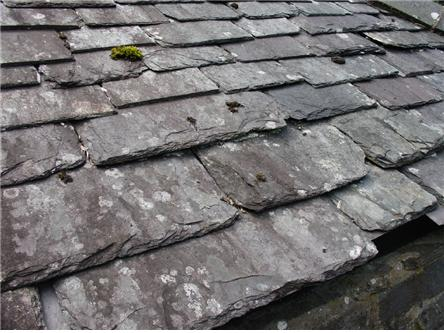
\includegraphics[width=0.8\textwidth]{./fig/slate_0001.jpg}
				\end{center}


		%		\tabulinesep=0.6ex
				\begin{tabu} to 1.0\textwidth { X[l, 1.0] X[l, 3.0] }
				\tabucline[0.2ex]{-}		
				화학  조성		&이질암.\\
				특징				&운모 (흑운모, 백운모), 근청석, 홍주석 등.\\
				광물  조성		&암회색을 띄며, 표면이 반짝거림. 벽개가 잘 발달하여 잘 쪼개짐.\\
				산      출		&이질암의 광역 변성 작용 초기에 형성됨.	\\
				모      습		&반점상 슬레이트\\
				\tabucline[0.1ex]{-}		
				\end{tabu} 

		\clearpage 
		
			점판암은 진흙이 땅 속에서 압력을 받아 굳은 것으로, 검은색 또는 회색의 돌로 얇게 쪼개지므로 지붕의 천연 슬레이트, 외벽, 마루 등에 많이 쓰인다.	\\
			
			셰일이 변성을 받아 형성된 흑색의 변성암, 지붕용 슬레이트, 벼루, 숫돌, 한옥 기와, 구들장으로 이용된다. \\

 
			점토가 굳어서 된 흑색의 치밀한 암석으로 입자의 크기가 작아 육안으로 구별이 되지 않는다. 
			쪼개짐이 특히 잘 발달되어 있어 평행한 얇은 판으로 잘 쪼개진다. 슬레이트라고도 부르며, 이암이나 셰일이 변성 작용을 받아 형성된 변성암이다. 
			그러나 변성 정도가 약해서 재결정 작용이 거의 일어나지 않은 채 쪼개짐만 발달한 것이다. \\

			점판암의 쪼개짐은 편리와 관계없이 발달하며, 때로는 편리와 직각으로 나타나기도 한다. 
			이와 같이 얇은 석판으로 잘 쪼개지기 때문에 건축용 재료로 많이 이용되고 있다. 
			점판암에는 운모(백운모, 흑운모), 홍주석, 석영, 장석, 탄산칼슘 성분 등이 포함되어 있어서 암회색을 띄며 표면이 반짝거린다. 	\\

			









	\clearpage
%	----------------------------------------------------------------------------------------------------------------------- section			천매암
	\section{천매암 千枚巖 Phyllite   }
	


		\subsection{첨매암 phyllite  千枚岩 요약 }

				암석의 조직이나 구조로 보아, 점판암과 결정편암의 중간적인 성질을 가진 변성암으로 매우 세립이지만 편리는 두드러진다. 
				때로는 변성 재결정 작용 때에 생긴 줄무늬 구조를 나타내어, 편리를 옆에서 보면 색의 차이로 생기는 줄무늬를 볼 수 있다.  


				
				\begin{center}
				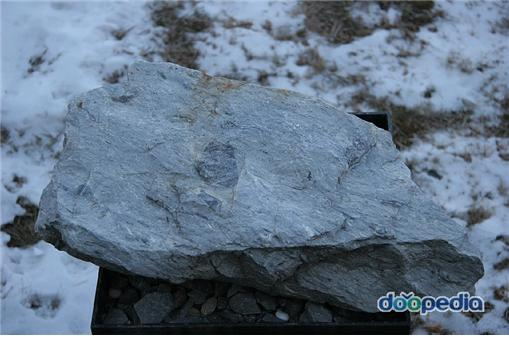
\includegraphics[width=0.8\textwidth]{./fig/Phyllite_0002.jpg}
				\end{center}
				담회색 천매암


				\begin{center}
				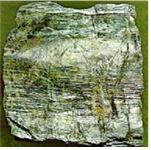
\includegraphics[width=0.8\textwidth]{./fig/Phyllite_0001.jpg}
				\end{center}


		%		\tabulinesep=0.6ex
				\begin{tabu} to 1.0\textwidth { X[l, 1.0] X[l, 3.0] }
				\tabucline[0.2ex]{-}		
				화학조성	&
				이질암.	\\
				특징	&
				석영, 견운모질 운모, 녹니석, (알바이트, 인회석, 전기석, 황철석, 자철석, 적철석, 일메나이트, 흑연 등).	\\
				분류	&
				동력변성암	\\
				산지	&
				충남 온양	\\
				광물조성	&
				무늬가 있고, 녹흑색, 흑색을 띄며 약간 만곡된 엽리를 보인다. 개개의 엽리는 육안으로 구분 불가능하며, 매우 적은 입자들로 구성되어 있다.	\\
				산출	&
				찰흙이 퇴적되어 있는 곳에 약간 강한 압력과 열의 영향(변성작용)을 받아서 생성된 암석이다. 	\\
				모습	&
				석영을 많이 포함한 천매암.	\\
				\tabucline[0.1ex]{-}		
				\end{tabu} 






		\subsection{천매암 어원}

				Phyllite는 ‘잎(Phyll-: 잎의 뜻을 가진 결합사) 모양의 암석’을 뜻한다. 
				이 암석에 대한 한국어와 조선어는 천매암, 일본어와 중국어는 千枚岩이며, ‘수없이 많은 얇은 잎이 겹쳐진 모양으로 된 암석’을 뜻한다.



		\subsection{천매암 성인과 특징}

				셰일의 광역변성과정 중 점판암과 편암 사이에 해당한다. 

				암석 표면에는 작은 주름과 엽리(葉理, foliation)가 수없이 많이 발달되어 있고 석영, 장석, 백운모, 견운모, 녹니석과 같은 광물 결정이 압력 방향에 수직으로 재결정되어 배열되어 있다.

				점판암 → 천매암 → 편암 → 편마암으로 조직이 변화한다. 


		\subsection{천매암}

				매우 세립(細粒)이지만, 편리(片理)는 두드러진다. 
				때로는 변성 재결정 작용 때에 생긴 줄무늬 구조를 나타내어, 편리를 옆에서 보면 색의 차이로 생기는 줄무늬를 볼 수 있다. 
				보통은 점토질 또는 이질(泥質)의 퇴적암에서 비롯된 흑색인 것이 많으며, 그것은 석영 ·장석 ·백운모 ·녹니석 ·방해석 ·석묵 등으로 되어 있다. 
				흔히 원래의 퇴적암의 사립(砂粒) 등을 많이 함유하고 있다. 
				한편, 응회암을 원암(原岩)으로 하는 녹색인 것도 있는데, 석영 ·장석 ·녹니석 ·설석(楔石) ·방해석 등으로 되어 있다. 
				이 경우에도 원래의 암석인 휘석이 잔류광물(殘留鑛物)로서 함유되어 있다. 
				일반적으로 이질암에서 비롯된 변성암은, 변성온도가 높아져서 재결정 작용이 진행함에 따라 점판암 → 천매암 → 편암 → 편마암으로 조직이 변화한다. 










	\clearpage
%	----------------------------------------------------------------------------------------------------------------------- section    편암
	\section{편암 片巖 Schist   }



				\begin{center}
				\includegraphics[width=0.8\textwidth]{./fig/schist_0001.jpg}
				\end{center}


		%		\tabulinesep=0.6ex
				\begin{tabu} to 1.0\textwidth { X[l, 1.0] X[l, 3.0] }
				\tabucline[0.2ex]{-}		
				화학  조성		&\\
				특징				&\\
				광물  조성		&\\
				산      출		&\\
				모      습		&\\
				\tabucline[0.1ex]{-}		
				\end{tabu} 



	\clearpage   \vskip 4em

		\subsection{편암 片岩, Schist }

				변성 퇴적암 
				
				엷은 판 모양으로 쪼개지는 성질(片理 또는 劈開)을 가진 변성암을 총칭하기도 한다. 
				
				
				결정이 성장하여 광물을 육안으로 관찰할 수 있을 정도의 엽리를 보일 때 이를 【 편리 】라 하며, 이러한 편리 구조를 보이는 암석을 편암이라 한다.

		\subsection{어원}
				
				Schist는 ‘쪼개지는’을 뜻하는 그리스어 schistos에서 유래. \\
				이 암석에 대한 한국어와 조선어는 편암, 일본어와 중국어는 片岩이며. ‘얇게 쪼개진 암석’을 뜻한다.
				
				
		\subsection{성인}
				
				화성암이나 퇴적암이 지하에서 심한 열과 압력을 받아 조암 광물들이 압력 방향에 수직 방향으로 재배열된 변성암이다. 
				원암의 종류에 따라 다양한 편암이 만들어진다.
				
				
		\subsection{용도}
		
				
				토목건축 재료
				[네이버 지식백과] 편암 [片岩, Schist] (기본 광물·암석 용어집, 2010.11.15, 한국학술정보(주))
				
				
				\begin{figure}
				\centering
				\caption{운모 편암}
				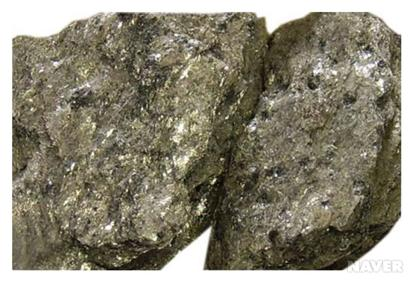
\includegraphics[width=0.8\textwidth]{./fig/schist_0002.jpg}
				\end{figure}
				
				
				\begin{figure}
				\centering
				\caption{장석 편암}
				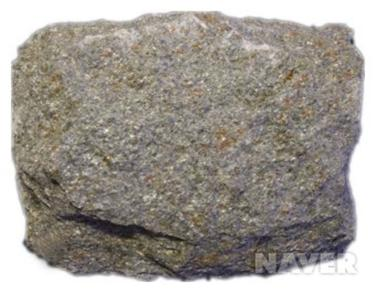
\includegraphics[width=0.8\textwidth]{./fig/schist_0003.jpg}
				\end{figure}
				
				
				
				




















	\clearpage
%	----------------------------------------------------------------------------------------------------------------------- section
	\section{편마암 片麻岩  gneiss }
	


			검은색과 흰색의 교호하는 물무뉘(면구조)가 있다.


				\begin{figure}[h]
				\centering
				\caption{편마암}
				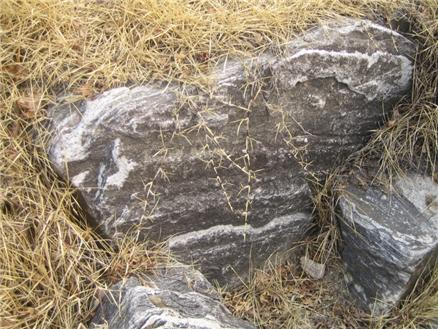
\includegraphics[width=0.8\textwidth]{./fig/gneiss_0001.jpg}
				\end{figure}



				\begin{figure}[h]
				\centering
				\caption{편마암}
				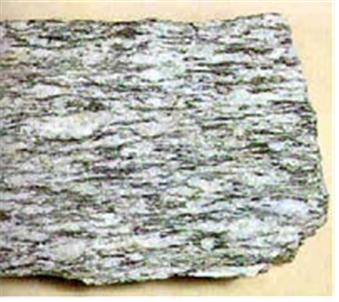
\includegraphics[width=0.8\textwidth]{./fig/gneiss_0002.jpg}
				\end{figure}



		%		\tabulinesep=0.6ex
				\begin{tabu} to 1.0\textwidth { X[l, 1.0] X[l, 3.0] }
				\tabucline[0.2ex]{-}		
				화학조성		&				규장질 내지 이질암. \\
				특징			&				장석 (미사장석 내지 퍼싸이트), 사장석 (알바이트 내지 올리고클래스), 석영, 운모 (흑운모, 백운모), (녹염석, 전기석, 저어콘 등).\\
				분류			&				동력변성암 \\
				산지 		&				전국 \\
				광물조성 		&				화강암 내지 정사암으로부터 형성된 것은 밝은색을 띄나, 이질 성분이 증가할 수록 흑운모 양의 증가로 어두운 색을 띈다. 편마구조를 잘 보인다.  \\
				산출 		&				조립질 암석이 영향을 받아서 구성 광물들이 압력에 수직방향으로 길게 재 배열된 암석의 일종이다. \\
				모습 		&				흑운모 편마암 \\
				\tabucline[0.1ex]{-}		
				\end{tabu} 







		\subsection{편마암}

				변성암의 일종으로, 이질(泥質) 또는 사질(砂質)의 퇴적암이 높은 온도 하에서 광역변성작용을 받은 경우에 생성된다.\\
%				[네이버 지식백과] 편마암 gneiss, 片麻岩 (두산백과)

				어두운색 광물과 밝은색 광물이 교대로 줄무늬를 이루는 편마암의 줄무늬는 암석이 지하 깊은 곳에서 높은 압력을 받으면서 광물들이 압력과 직각인 방향으로 다시 배열되어 만들어 진 것이다.



		\subsection{어원}
		

				Gneiss의 어원은 아직 정확하게 밝혀지지 않았지만 ‘광채가 나는’을 뜻하는 11 $\sim$ 14세기의 독일어 gneist에서 유래한 것으로 알려져 있다. \\
				
				이 암석에 대한 한국어와 조선어는 편마암, 일본어와 중국어는 片麻岩이며, ‘얇게 쪼개진 삼 모양의 암석’을 뜻한다. 
				마(麻)는 대마의 줄기를 발효시켜 섬유다발로 만든 삼이다.\\
				
				[네이버 지식백과] 편마암 [片麻岩, Gneiss] (기본 광물·암석 용어집, 2010.11.15, 한국학술정보(주))







	\clearpage   \vskip 4em

		\subsection{편마 구조}
		

				【 유색광물 】과 【 무색광물 】이 서로 교대로 거친 줄무늬를 보여주는 것을 【 편마(片麻)구조 】라 한다.
				
				편암이 만들어지는 변성온도와 압력보다 더 높은 조건에서는 광물들이 재결정되면서 크기가 커지고, 또 흑운모와 각섬석 같은 【 검은색 계열의 유색광물 】과 석영, 장석 등으로 이루어진 【 흰색 계열의 무색 광물 】이 
				서로 다른 부분으로 나뉘어져 검은 색 띠와 흰색 띠를 형성하는 데 이를 【 편마 구조 】라고 한다. 
				이렇게 편마구조를 보이는 변성암을 【 편마암 】이라 한다. 
				
				이 편마암은 정원석으로 자주 사용되는 암석으로 우리나라에도 매우 넓게 분포한다. 또한 우리나라에 분포하는 다른 암석보다 비교적 먼저 만들어졌기 때문에 우리나라의 기반암을 형성하고 있다.
	




				
	\clearpage   \vskip 4em
				
		\subsection{성인과 조직}

				화성암이나 퇴적암이 지하에서 심한 열과 압력을 받아 조암 광물들이 압력 방향에 수직으로 재결정된 변성암이다. 
				원암과 변성 조건에 따라 특징적인 변성 조직이 생긴다. 
				그 조직의 모양에 따라 안구상 편마암(眼球狀片麻岩, Augen Gneiss), 호상 편마암(縞狀片麻岩, Banded Gneiss), 화강 편마암(花崗片麻岩, Granite Gneiss)으로 구분된다.\\
%				[네이버 지식백과] 편마암 [片麻岩, Gneiss] (기본 광물·암석 용어집, 2010.11.15, 한국학술정보(주))



				①  안구상 편마암
				② 호상 편마암
				③ 화강 편마암
				
				
				편암이나 편마암은 풍화에 비교적 잘 견디지만, 화강암은 풍화에 약하여 쉽게 토양으로 변한다.
				





	\clearpage   \vskip 4em
				
		\subsection{편마암의 구분}

				이 편마암은 【 퇴적암류 】에서 변형된 것과 【 화성암류 】에서 변형된 것으로 나눌 수 있다.


				\begin{figure}[h]
				\centering
				\caption{편마암 : 검은색과 흰색의 교호하는 물무뉘(면구조)가 있다.}
				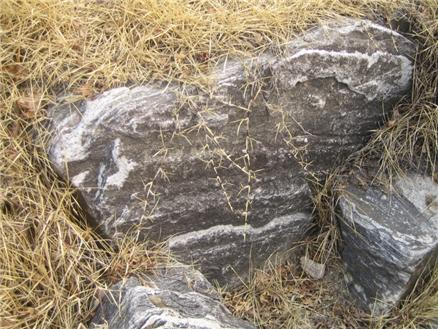
\includegraphics[width=0.4\textwidth]{./fig/gneiss_1003.jpg}
				\end{figure}




				\begin{figure}[h]
				\centering
				\caption{편마암 : 검은색과 흰색의 교호하는 물무뉘(면구조)가 있다.}
				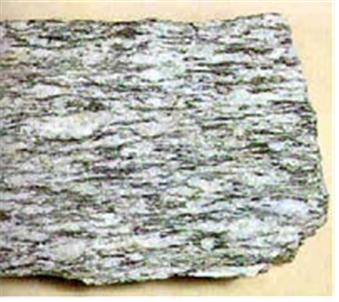
\includegraphics[width=0.4\textwidth]{./fig/gneiss_1004.jpg}
				\end{figure}




		\subsection{화강 편마암 granite gneiss, 花崗片麻岩, 花崗片麻巖  }

				외국어 표기 花崗片麻岩(한자), granite geniss(영어) 
				동의어 결정편마암(正片麻岩), 정편마암 
				
				화강 편마암이란 화강암이 변성 작용을 받아서 형성된 편마암이다.
				
				변성암의 일종으로 화강암이 【 동력 변성 작용 】을 받아서 생성된 것이다. 
				
				
				육안으로는 화강암과 유사하나, 성분이 층상으로 배열되고 편상구조(片狀構造)를 이루고 있는 것으로 구별한다. 정편마암(正片麻岩) 또는 결정편마암이라고도 한다.  \\
				
				[네이버 지식백과] 화강편마암 [granite gneiss, 花崗片麻岩, 花崗片麻巖] (용어해설)


		\subsection{압쇄 편마암}

				양원리 하천가에 분포하는 람석은 어두운색광물과 밝은색 광물이 교대로 줄무늬를 이루는 편마암으로, 본래 이 암석은 선캄브리아시대에 만들어졌다. 
				
				편마암의 줄무늬는 암석이 지하 깊은 곳에서 높은 압력을 받으면서 광물들이 압력과 직각인 방향으로 다시 배열되어 만들어진 것이다.
				
				이곳의 암석은 자세히 보면 보통의 편마암과는 다르게, 밝은색을 띠는 장석 광물이 마치 사람의 눈과 같이 둥근 모양을 하고 있다. 
				이런 형태의 장석을 어떻게 만들어졌을까? 손바닥에 진흙이 묻어 있을 때 진흙은 납작하게 눌림과 동시에 동그랗게 말린다. 
				이곳 암석도 지하 깊은 곳에 있을 때, 양쪽에서 누르며 미는 작용을 받은 것이다. 
				이런 변성작용을 전단작용( 압쇄암화작용 또는 파쇄변성작용 ) 이라고 한다. 
				그래서 이곳의 암석을 【 압쇄편마암 】이라고 한다,.
				
				

































	\clearpage
%	----------------------------------------------------------------------------------------------------------------------- section
	\section{한반도의 편마암}



		\subsection{한반도의 편마암}

			정원 조경석으로 사용되는 편마암은 고생대보다 더 오래된 원생대(선캄브리아)의 암석으로 한반도 땅덩어리가 아주 오랜 역사를 지녔음을 말해준다.

		\subsection{한반도의 편마암}

				흰색과 검은색 물무늬가 물결처럼 이어지며 층을 이루고 있는 이 암석은 【 선캄브리아대 】 【 변성암 】으로 【 마그마타이트(migmatite)질 편마암 】이다. 
				이것은 지하의 고온과 고압에 의해 퇴적암이 변성을 받을 때 암석에 섞여 있던 광물들이 녹은 뒤 같은 종류끼리 다시 모이는 【 재결정 작용 】으로 형성되었다.

				【 석영 】, 【 장석 】 등의 밝은색 광물은 흰줄, 【 흑운모 】와 같은 어두운 색 광물은 검은 중 모양으로 뒤엉켜 있다. 
				마치 나뭇잎을 포개놓은 모양 같아 이를 지질학 용어로 【 엽리 】(엽리, foliation)라 하는데, 
				그 구조가 서로 달라 풍화와 침식에 약한 흑운모 성분이 먼저 떨어져 나가고, 침식에 강한 석영 성분은 상대적으로 높은 곳에 있게 된다. 
				그 결과 기반암이 울통 불퉁한 굴곡을 이루게 되었는데 이는 손으로 만져보면 누구나 쉽게 알 수 있다.



		\subsection{한반도의 편마암}

				한반도에서 발견된 암석 가운데 가장 오래된 것은 약 30억 년 전에 형성 된 【 편마암 】으로, 이를 통해 우리는 한반도의 탄성 연대를 어림잡아 볼 수 있다. 

				선캄브리아대 암석의 대부분을 차지하는 편마암은 지구가 탄생하고 바다가 만들어진 후 원시 바다에서 형성된 퇴적암이 지하 깊은 곳에서 열과 압력을 받아 변성된 것으로 
				고생대 이전에는 한반도가 바다였다는 사실을 보여주는 암석이라고 할 수 있다.

				선캄브리아대 편마암이 분포하는 지역은 【 평북개마지괴 】, 【 경기지괴 】, 【 영남(소백산)지괴 】로 국토의 40\% 정도를 차지한다. 
				그러므로 한반도 땅덩어리는 고생대 이전에 이미 대략적인 윤곽을 갖추었으리라 추정해 볼 수 있다.,


				\begin{figure}[h]
				\centering
				\caption{한반도의 지괴}
				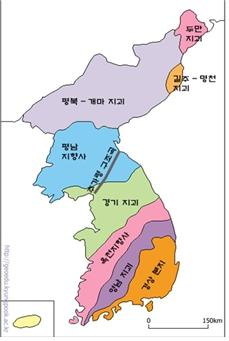
\includegraphics[width=0.4\textwidth]{./fig/gneiss_1002.jpg}
				\end{figure}

				선캄브비아대에는 전 세계적으로 조산 운동은 거의 일어나지 않았고, 주로 지표가 깎여나가는 침식 작용이 일어났다. 
				당시 원시 바다에 떠 있던 초대륙의 일부였던 한반도 역시 큰 지각 변동은 없었고, 지표의 침식으로 방패 모양의 평탄 지형을 이루고 있었다. 
				그러나 이후 선캄브리아대의 암석들이 고생대, 중생대, 신생대를 거치며 여러 차례의 지각변동과 화성 활동으로 심하게 변성되어, 한반도의 지질 구조는 매우 복잡해졌다. 
				게다가 화석이 거의 발견되지 않아 지층의 선후 관계를 밝히기도 대단히 어려운 실정이다.





	\clearpage
%	----------------------------------------------------------------------------------------------------------------------- section
	\section{구상 편마암 片麻岩  gneiss }





		\subsection{구상 편마암}

				변성암 중에서 다소 특이한 형태를 보이는 것이 바로 광물들이 둥글게 동심원 모양을 만들면서 나타나는 【 구상 편마암 】이다. 

				이러한 구성 구조는 경북 상주의 구상 화강암처럼 화성암에서도 나타난다고 한다. 
				이 구상편마암은 전북 무주 부근에서 발견되는데, 천연기념물로 지정되어 있고, 수석의 가치도 비교적 크다고 한다. 
				이 구상편마암은 변성 전 물질이 퇴적암류가 아인 화강암으로 생각되므로 화강편마암의 일종리라고 말할 수 있다.



	\clearpage   \vskip 4em

		\subsection{무주 오산리 구상 화강 편마암}

				무주화강 편마암에 대한 권용안 등(1995)의 연구에 의하면, 
				화강암에 포획되어 있던 이질기원의 퇴적암이 열과 압력에 의한 변성작용을 받게 되고, 
				그로 인해 새로운 광물들이 이 퇴적암을 중심으로 동심원상으로 만들어지면서 이러한 구상구조가 형성된 것이라고 한다. 
				구상구조의 모양은 동심원 형태와 길쭉하게 한 방향으로 늘어난 형태로 구분할 수 있다. 
				구상구조의 암녹색 핵을 이루고 있는 광물은 근청석, 규선석, 흑운모 등이고, 핵을 둘러싸고 있는 어두룬 색의 껍질은 흑운모, 녹리석, 전기석, 그리고 밝은 색의 껍질은 사장석, 석영, 소량의 정장석 등으로 구성되어 있다. 
				구상 구조들 사이의 암상은 물론 화강 편마암이다.





				무주 오산리 구상화강편마암은 전라북도 무주군 무주읍 오산리에 있는, 화강편마암에 생긴 구상암(球狀巖)이다. 
				대한민국의 천연기념물 제249호로 지정되어 있다.

				공처럼 둥근 암석인 구상암은 대부분 화강암 속에서 발견되는데, 전 세계적으로 100여 곳에서만 발견되었으며, 한국에서는 5곳에서 발견되었다. 
				무주 오산리 구상화강편마암의 둥근 핵은 지름이 5∼10㎝이고 색깔은 어두운 회색이거나 어두운 녹색이다. 
				이 구상암은 화강암이 아닌 변성암 속에 있어 매우 희귀한 경우에 속하여 학술적으로 대단히 중요한 가치를 지닌다.








				\begin{figure}
				\centering
				\caption{구상 화강 편마암}
				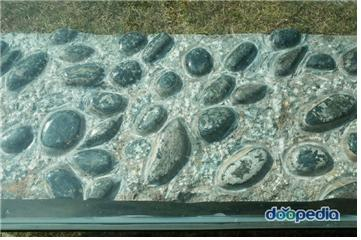
\includegraphics[width=0.8\textwidth]{./fig/gneiss_1001.jpg}
				\end{figure}











	\clearpage
%	----------------------------------------------------------------------------------------------------------------------- section
	\section{규암  硅巖 Quartzite  }




				\begin{figure}[h]
				\centering
				\caption{규암}
				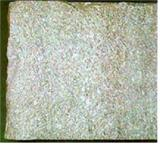
\includegraphics[width=0.4\textwidth]{./fig/Quartzite_0001.jpg}
				\end{figure}



				\begin{center}
				\end{center}



		%		\tabulinesep=0.6ex
				\begin{tabu} to 1.0\textwidth { X[l, 1.0] X[l, 3.0] }
				\tabucline[0.2ex]{-}		
				화학조성		&규질. \\
				특징			&주로 석영으로 구성되어 있으며 약간의 운모 (흑운모, 백운모)나 장석이 있을 수 있다. \\
				분류			&열 변성암\\
				산지			&충묵 옥천 \\
				광물조성		&대개 밝은 색을 띄며, 괴상이나, 운모의 양이 증가하면 쪼개짐을 잘 보이기도 한다. \\
				산출			&점판암과 사암이 관입된 마그마의 열에 의하여 생성된 암석으로 흰색의 유리와 같은 알갱이로 되어 있다.  \\
				모습			&은회색의 규암 \\
				\tabucline[0.1ex]{-}		
				\end{tabu} 



	\clearpage   \vskip 4em

		\subsection{규암}
		

				규소 규(硅) 바위 암(岩)
				
				사암(모래의 퇴적)이 열과 압력을 받은 변성암
				
				규암은 퇴적암의 일종인 【 모래가 쌓여 굳어진 사암 】이 【 열과 압력에 의한 변성 】을 받을 경우 만들어 지는 암석이다. 
				
				규암의 구성 광물은 주로 【 재결정된 석영 】인데, 이 석용은 다른 광물에 비해 비교적 단단하기 때문에 규암끼리 강하게 부딫칠 경우 불꽃이 튄다.


		\subsection{규암의 생성}

				규암은 원래 입자가 매우 고문 모래가 퇴적 작용을 받아 형성된 사암이었다. 그러다 지각 변동에 의해 사암이 지하 깊은 곳으로 들어간 후, 높은 열과 압력으로 변성작용을 받으면서 규암으로 바뀐 것이다.
				
				규암은 모래가 퇴적작용을 받아 형성되는 사암이 지각변동으로 땅속 깊은 곳으로 끌려들어간 후 높은 온도와 압력에 의해 변성작용을 받아 형성된 변성암으로 매우 단단하고 치밀하다.



	\clearpage   \vskip 4em

		\subsection{규암의 모양}


				\begin{figure}[h]
				\centering
				\caption{규암의 모양}
				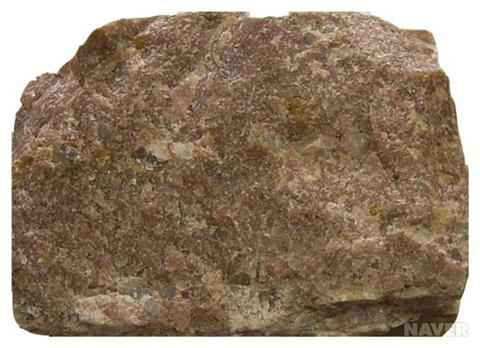
\includegraphics[width=0.8\textwidth]{./fig/Quartzite_0002.jpg}
				\end{figure}

	\clearpage   \vskip 4em

		\subsection{규암의 특징}

				암석은 광물로 이루어지는데 규암은 광물 중에서도 매우 단단한 편에 속하는 석영으로 되어 있다.( 모래의 퇴적으로 형성 ) 
				따라서 규암은 암석 중에서도 단단한 편에 속한다. 이러한 이유로 규암은 침식이나 풍화 작용에 매우 강하여 쉽게 부서지거나 풍화되지 않는 특징을 가진다.


		\subsection{판상 규암층}
		

























	\clearpage
%	----------------------------------------------------------------------------------------------------------------------- section
	\section{대리암  大理巖 Marble   }


		\subsection{대리암 요약}

			변성암 중에는 구성광물이 비교적 단순한 경우도 있는데, 그 예로는 대리암과 규암을 들수 있다. \\
			
			대리암은 【 석회암 】이 열 변성이나, 열과 압력에 의한 변성을 받았을 때 만들어지는 암석으로 재결정된 커다란 【 방해석 네모로 잘 갈라지는 광물을 뜻한다 】 결정이 특징적이며, 고급 건축재로 많이 사용된다.
			
				\begin{center}[h]
				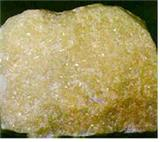
\includegraphics[width=0.8\textwidth]{./fig/Marble_0001.jpg}
				\end{center}
			

	\clearpage   \vskip 4em

		\subsection{대리암}

			대리석이라고도 한다. 변성암 중의 하나로 석회암이 오랫동안 열변성 작용을 받아 만들어진 것이다. 
			암석을 이루는 주된 광물은 방해석이며, 드물게는 흑연이나 황철석 등이 함께 발견되기도 한다. 
			때로는 고회석, 석영, 운모류, 녹니석, 사장석, 활석, 사문석 등이 함께 산출되기도 한다. 
			
			겉보기 색은 흰색, 녹색, 회색, 갈색, 붉은색 등 다양하다. 대리암은 암석을 이루는 알갱이가 특정 방향으로 배열되어 있지 않으므로 엽리 조직은 볼 수 없다. 
			
			석회암이 변성 작용을 받으면 결정질석회암이 되며, 결정질석회암이 변성 작용을 더 받으면 대리암이 된다. 
			대리암의 조직은 입상 변정질이라는 조직과 다이아블라스틱이라는 조직이 나타나는 것이 특징인데, 입상 변정질 조직은 암석을 이루는 알갱이의 크기가 거의 같은 조직이다. 
			서로 크기가 같아서 경계도 없고 알갱이가 이루는 방향도 없다. 
			또 다이아블라스틱 조직은 바늘이나 판 모양 편리를 형성하지 않고 서로 맞닿아 있어 부분적으로는 사방으로 퍼지는 방사형을 이룬다. 
			대체로 덩어리 상태로 산출되며 암석을 이루는 알갱이의 크기는 작은 것부터 큰 것까지 다양하다. 
			
			대리암은 석회암 변성 지대에 폭 넓게 분포한다. 이탈리아 북서부 토스카나주 카라라라는 도시에서 생산되는 대리석은 미켈란젤로의 조각 재료로 이용된 것으로 유명하다. 
			또 미국의 알라바마 주에서는 60m 두께의 대리암이 산출되기도 하였다. 
			미국의 버몬트에서는 130km나 되는 긴 대리암 층이 발견되었다. 
			대리암은 무늬가 아름다워 조각 재료로 이용되며 건물의 내부 장식 재료로 이용된다.
			

		%		\tabulinesep=0.6ex
				\begin{tabu} to 1.0\textwidth { X[l, 1.0] X[l, 3.0] }
				\tabucline[0.2ex]{-}		
				화학조성		&탄산염암.\\
				특징			&주로 방해석 및 돌로마이트 등의 탄산염 광물로 구성되어 있으나, 석영, 투각섬석, 양기석, 금운모, 투휘석 등이 존재하기도 한다.\\
				분류			&열변성암 \\
				산지			&경기, 충북 \\
				광물조성		&불순물의 종류에 따라 틀리나 밝은 회색 내지 황색을 띈다. \\
				산출			&변성과정중에 유색광물의 함유나 석회암의 생성과정에서 성분이 순순하지 못한 암석이 마그마의 열에 의하여 변질 생성된 암석이다. \\
				모습			&주로 돌로마이트로 구성된 대리암 \\
				\tabucline[0.1ex]{-}		
				\end{tabu} 



































	\clearpage
%	----------------------------------------------------------------------------------------------------------------------- section
	\section{	운모 편암 雲母 片岩 mica schist }	



				\begin{center}
				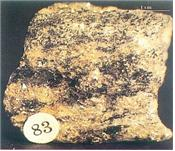
\includegraphics[width=0.8\textwidth]{./fig/mica_schist_0001.jpg}
				\end{center}





주구성광물
흑운모 ․백운모 ․석영 ․칼륨장석 ․사장석 등
특징
점토질 암석이 지하의 온도 ․압력을 받아 변성된 것이다. 운모류는 결정의 밑면이 최대 편압방향으로 향한 평행구조를 가지며, 편상 조직이 뚜렷하다. 
분류
동력변성암
산지
전국
광물조성
불순물의 종류에 따라 틀리나 밝은 회색 내지 황색을 띈다.
산출
세립질 암석 사암, 혈암, 퇴적암이 압력을 받거나 운모와 같은 판상의 광물이 재결정 작용을 받아서 변질되어 생성된 암석이다.
모습
흑운모를 많이 함유한 것은 암적갈색인데, 백운모의 함유량이 많아질수록 색이 엷어진다. 넓은 면에 나뭇잎같은 구조가 있다.




	\clearpage
%	----------------------------------------------------------------------------------------------------------------------- section
	\section{	혼펠스 Hornfels }
	

결정 크기가 작은 세립질 변성암을 통틀어 일컫는 말로, 깨진 부분이 모가 난 뿔같다고 하여 각암이라고도 한다. 셰일이나 이암이 열변성 작용을 받아 만들어진 변성암이다. 조직을 관찰해 보면 암석을 이루는 알갱이의 크기가 비슷하고 방향성이 없으므로 엽리 조직같은 줄무늬가 보이지 않는다. 겉보기 색은 흰색, 분홍색, 갈색, 보라색, 녹색이며, 알갱이가 모여 있는 곳마다 서로 다른 색을 띤다. 

혼펠스는 크게 세 종류가 있으나 이질 퇴적암이 변성되어 만들어진 혼펠스가 가장 대표적이며, 염기성 화성암이 열변성 작용을 받아 혼펠스가 만들어지기도 한다. 이질 퇴적암이 변성되어 만들어진 혼펠스에는 흑운모, 홍주석, 근청석, 정장석 등이 들어 있으며, 높은 열변성 작용을 받았을 때는 규선석, 사방휘석, 석류석도 발견된다.

				\begin{center}
				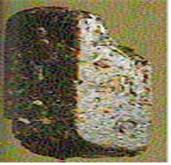
\includegraphics[width=0.8\textwidth]{./fig/Hornfels_0001.jpg}
				\end{center}



화학조성
원암의 종류에 따라 다르다.
특징
원암의 종류에 따라 다름.
광물조성
이질암이 접촉 변성을 받았을 경우는 대개 검은색을 띠며 치밀하다. 탄산염암이 접촉 변성을 받았을 경우는 연녹색을 띄며 투각섬석 및 투휘석 등의 석회 규산염광물이 관찰되기도 한다.
산출
화성암의 관입과 같은 것으로 인한 급격한 열변성을 받아 형성된다.
모습
이질암 기원의 호온펠스



	\clearpage
%	----------------------------------------------------------------------------------------------------------------------- section
	\section{흑운모 편마암}
	

	\clearpage
%	----------------------------------------------------------------------------------------------------------------------- section
	\section{각 섬 암}
	


	\clearpage
%	----------------------------------------------------------------------------------------------------------------------- section
	\section{감 람 암}
	



	\clearpage
%	----------------------------------------------------------------------------------------------------------------------- section
	\section{사 문 암}
	


	\clearpage
%	----------------------------------------------------------------------------------------------------------------------- section
	\section{비 눗 돌}
	


	\clearpage
%	----------------------------------------------------------------------------------------------------------------------- section
	\section{미그마타이트}
	

















%% 	======================================================================================================================= part  퇴적암
	\addtocontents{toc}{\protect\newpage}	
	
	
		\part{퇴적암}
	





	
	
% 	======================================================================================================================= chapter
	\clearpage
	\chapter{퇴적암 일반 \\ sedimentary rock}
	\minitoc				% Creating an actual minitoc
	


	\clearpage
%	----------------------------------------------------------------------------------------------------------------------- section
	\section{퇴적암 개요}

		\paragraph{}
		육지 표면에 분포되어 있는 암석의 75\%는 퇴적암 내지 변성퇴적암으로 이루어져 있고 
		나머지 25\%만이 화성암 내지 화성기원의 변성암으로 되어 있다.

		학자들이 바닷물에 들어 있는 Na(화성암에서 유래된 것으로 추정)의 양 및 기타 또 다른 근거로부터 계산한 바에 의하면 
		육상의 퇴적암층의 평균 두께는 1.5 km 이다.

		그러므로 육지 표면의 4분의 3을 덮고 있는 퇴적암도 지하로 들어감에 따라 그 양이 감소될 것이며 
		해양지각에 가까이 가면 거의 퇴적암을 찾아볼 수 없을 것이다.

		퇴적암은 지각의 표면에 겹겹이 층리를 가지며 얇게 붙어 있는 껍질이라고 생각 할 수 있다.


		\paragraph{}
		퇴적암은 지구의 역사 즉 지사의 연구에 꼭 필요한 암석으로, 
		지질학자들은 이 퇴적암층을 조사하여 수억 년 전부터 지금까지의 지사를 알아내려고 노력하고 있다. 
		지층이 간직한 모든 사실들이 정확하게 해석된다면 우리는 지구의 과거를 자세히 알 수 있을 것이다. 
		뿐만 아니라 퇴적암의 지층 내에 존재하는 화석을 연구함으로써 지구상에 서식했던 생물과 그 진화의 모습 및 현재의 생물에 대한 기원을 밝힐 수 있다.











	\clearpage
%	----------------------------------------------------------------------------------------------------------------------- section
	\section{퇴적암 개요}

			지구표면의 암석이 상온 ·상압 하에서 풍화작용으로 분해 ·이동되어 지구 표면에 침적하는 퇴적작용으로 생긴 암석.
			
			지표에 노출된 암석은 풍화 및 침식작용을 받아 암설 또는 수용액으로 되어 원암에서 분리되는데 
			이렇게 분리된 물질과 생물의 유해가 육상 또는 수저에 쌓여서 만들어진 암석이 퇴적암이다. 
			
			암석이 풍화나 침식을 받아 부서져서 만들어진 자갈이나 모래, 진흙, 화산재, 물에 녹아 있던 물질 등이 쌓인 것을 【 퇴적물 】이라고 한다. 
			이러한 퇴적물이 쌓인 후 굳어져 생긴 암석을 【 퇴적암 】이라고 한다. 
			퇴적암은 암석을 이루는 퇴적물의 종류에 따라 나누며, 역암, 사암, 셰일, 석회암, 응회암 등이 있다.







	\clearpage
%	----------------------------------------------------------------------------------------------------------------------- section
	\section{퇴적암}

				일반적으로는 미고결(未固結) 상태의 것은 퇴적물이라 하고, 고결된 것만을 퇴적암이라고 부른다. 
				
				이에 대하여 수성암(水成岩)은 퇴적암의 대부분이 수성, 즉 수중에서 퇴적이 되기 때문에 
				화성암(火成岩)과 대립적인 수성암이란 말이 사용되는 것이다. 
				그러나 퇴적암에는 수중이 아닌 공기 중에서 퇴적되어 형성되는 것도 있다. 
				퇴적암에는 화성암이나 변성암에서는 볼 수 없는 특수한 성질이 있다. 그 하나는 지층을 형성하고 다른 하나는 때때로 화석을 함유한다.
				
				지구 표면에서 풍화된 암석의 부스러기는 물이나 대기를 매개물로 하여 운반되며, 중력에 의하여 보다 낮은 곳으로 이동된다. 
				물로 이동되는 방법에는 세 가지 종류가 있으며, 모래 알갱이 등의 조립질인 쇄설물은 기계적으로 유수(流水)에 의하여 밀려 내려가고, 
				점토광물과 같은 세립질 물질은 수중에 떠서, 나트륨 ·칼륨 ·마그네슘 ·칼슘 등은 물에 용해된 상태로 각각 운반된다. 
				그 결과 이들 물질은 바다나 호수 같은 곳까지 이동하여, 물의 흐름이 약해지거나 수소이온농도의 영향, 뚜렷한 증발현상 등에 의하여 
				각종 물질이 침전된다. 
				그리하여 어떤 넓이를 가진 평편한 지층(地層)으로 된다. 
				퇴적물은 그 지역의 지반의 침강과 더불어 점점 두껍게 쌓여 지층을 형성하면서 차례차례로 쌓여 마침내는 두꺼운 일련의 지층군을 만든다. 
				지층군은 그 당시의 지형이나 기후 등과 같은 환경이나 지각변동 등에 지배되어 어떤 특정한 퇴적암의 콤비를 이루며, 
				퇴적 당시의 생물의 유해나 유물 또는 그들 생물의 생활흔적 등을 남기기도 한다. 
				지층 중에 포함된 화석군(化石群)의 연구로 생물의 변천사를 명백히 추측할 수가 있다. 
				
				다른 한편으로는 수평으로 쌓인 지층이 습곡(褶曲)이나 단층(斷層)으로 서로 어긋나 있든지 하여 
				본래와는 많이 달라진 상태로 되어 있는 경우가 많다. 
				퇴적암에 반영된 지각 상층부의 변화는 지질구조나 지각변동의 성질 또는 역사를 판단하는 데 중요한 열쇠가 된다. 


	\clearpage
%	----------------------------------------------------------------------------------------------------------------------- section
	\section{퇴적암의 구성}

				퇴적암은 일반적으로 알갱이 상태의 광물 또는 암석의 파편과 이들 사이를 메우는 세립물질 등으로 구성되어 있다.
				
				전자는 쇄설물질이라 하며 지표의 암석이 침식 ·풍화로 생긴 자갈 ·모래 ·점토 등이다. 
				
				후자는 교결물질 또는 화학물질이며 보통은 퇴적 장소에서 형성된다.  \\
				
				이들과 같은 구성 물질 중에서 어떤 것이 중요한가에 따라서 【 쇄설성(碎屑性) 퇴적암 】과 【 화학적 퇴적암 】 등으로 구분한다. 
				이 밖에 생물의 유해가 쌓여서 된 것, 또는 그들의 생활과 관련되어 만들어진 퇴적암을 【 생물성 퇴적암 】이라고 한다. 
				

		%		\tabulinesep=0.6ex
				\begin{tabu} to 1.0\textwidth { X[l, 1.0] X[l, 4.0] }
				\tabucline[0.2ex]{-}		
				구분			&내용\\
				\tabucline[0.1ex]{-}		
				쇄설성퇴적암	&기존 암석 및 기타 다른 고형물의 깨진 부스러기가 쌓여 형성된 암석\\
				화학적퇴적암	&화학적 침전물이 퇴적되어 만들어진 암석\\
				유기적퇴적암	&과거 생존하던 생물의 유해가 쌓여서 만들어진 암석\\
				\tabucline[0.1ex]{-}		
				\end{tabu} 



% 	======================================================================================================================= chapter
	\clearpage
	\chapter{퇴적암의 생성 과정}
	\minitoc
	




	\clearpage
%	----------------------------------------------------------------------------------------------------------------------- section
	\section{퇴적암의 생성 과정}



		\paragraph{퇴적암의 생성 과정}


				\begin{itemize}[topsep=0.0em, parsep=0.0em, itemsep=0em, leftmargin=12.0em, labelwidth=3em, labelsep=3em] 
				\item [1.] 퇴적물의 기원
				\item [2.] 운반 및 퇴적
				\item [3.] 쇄설성 퇴적물
				\item [4.] 화학적 퇴적물
				\item [5.] 유기적 퇴적물
				\item [6.] 속성 작용
				\end{itemize}




	\clearpage
%	----------------------------------------------------------------------------------------------------------------------- section
	\section{퇴적물의 기원}


		지구의 태초, 퇴적암이 생성되기 전의 \textbf{원시 지각}은 화성암 내지는 운석 물질의 집합체 였을 것이다.
		이것이 풍화 및 침식을 받아 자갈, 모래 및 펄과 같은 쇄설물로 만들어져 이들이 물 밑에 쌓여서 최초의 퇴적암이 생성되었다.
		그 후 지각변동으로 생성된 이곳이 육화 되면서 물위에 나타나 퇴적암이 생성되었다. 
		풍화작용은 모든 암석을 지표로부터 파괴하여 여러 가지 \textbf{풍화 생성물}을 만든다. 
		이렇게 만들어진 풍화 및 침식에 의한 생성물은 강이나 호수 등의 물이나 빙하 혹은 바람 등에 의한 운반과 
		이들이 쌓이는 \textbf{퇴적 작용}을 거쳐 \textbf{고화 작용}을 받아 \textbf{퇴적암}으로 변한다.






	\clearpage
%	----------------------------------------------------------------------------------------------------------------------- section
	\section{퇴적물의 운반 및 퇴적}


			퇴적물은 쇄설성 퇴적물, 화학적 퇴적물, 유기적 퇴적물로 크게 나누어지며 이들은 각각 퇴적의 과정을 달리 한다.






	\clearpage
%	----------------------------------------------------------------------------------------------------------------------- section
	\section{쇄설성 퇴적물}

		쇄설성 퇴적물은 암에서 분리되어 처음부터 퇴적될 때까지 알갱이로 존재하다가 퇴적된 물질이다.
		원암으로부터 분리되어 운반되는 도중에 점차 마모되고 변형되어 
		운반 과정의 말기에는 최종적인 형태를 가진 펄에서 왕자갈까지의 크고 작은 입자들로 완성된다.

		이들은 그 크기에 따라 \textbf{환경에 대하여 안정한 위치}에 선택적으로 퇴적된다. 
		입자들의 직경 및 형태는 그들의 퇴적 속도와 퇴적 장소를 정하여 준다. 
		입자의 크고 원형에 가까운 곳은 바로 낙하하여 퇴적되므로 얕은 수저에 쌓이고, 
		직경이 작고 납작한 입자는 침하속도가 늦으므로 떠서 먼 곳까지 운반되어 깊은 곳에 퇴적된다.

		\paragraph{왕자갈}
		왕자갈은 사람의 머리보다 더 큰 돌덩이로서 약간 둥글게 되어 모서리가 없어진 것이다.
		모서리가 떨어지지 않고 예리한 모와 능선이 있는 큰 돌덩어리를 암괴라고 하여 구별한다.
		왕자갈과 잔자갈도 서로 부딪치고 달아서 둥글게 된 것을 말한다.

		학자에 따라서는 2 mm 이상 되는 입자를 자갈로 취급한다.
		그들에 의하면 왕모래는 자갈로 분류되나, 
		암석이 왕모래로 되어 있어도 이를 사암이라고 부르는 사람이 많으므로 
		왕모래를 모래의 일종으로 구분하는 것이 좋을 것으로 생각된다.

		자갈 왕자갈 잔자갈이라고 하면 장경이 2 mm 이상의 큰 알갱이 한 개 한 개를 의미하기도 하고 집합체를 의미하기도 한다.
		그러므로 한 개씩의 자갈을 강조하고 싶으면 '한 개의 자갈'이라고 하는 것이 좋을 것이다. 


		\paragraph{각력}
		모서리가 있는 자갈 크기의 덩어리에는 각력이라는 말을 쓰는데 이것은 집합체로서의 용어이다.
		각력이 굳어진 것이 각력암이다.


		왕모래와 모래에는 물속에서 대체로 모서리가 그대로 보존되어 있다. 
		이는 물의 입자들 사이의 완충 작용을 담당하여 입자들의 마찰을 피하게 하기 때문이다.
		이와 반대로 사막의 모래는 서로 충돌하여 둥글고, 표면은 우유빛 유리처럼 갈려 있다.
		모래는 풍화작용과 마찰에 대한 저항이 큰 광물들로 구성되어 있다.
		풍화에 대한 저항이 가장 큰 광물은 석영이므로 모래의 대부부분은 석영입자로 되어 있다.


		\paragraph{점토}
		세립의 모래 입자는 큰 입자들이 서로 충돌할때에 만들어진 작은 입자들과 2차적으로 생성된 입자들의 혼합으로 되어 있다.
		육안으로도 점토보다는 약간 거칠게 보이므로 점토와 구별이 가능하다.

		점토는 다른 광물이 화학적인 풍화작용과 속성작용으로 변하여 만들어진 2차적인 점토광물들로 되어 있다.
		점토의 주성분인 고령토의 입자는 극히 작으나 전자현미경으로 보면 극히 미세한 결정형으로 나타난다.







		\clearpage  \vskip  4em
		\subsection{쇄설성 퇴적물}

			\paragraph{1) 쇄설 (碎屑)}
				명사, 깨어진 부스러기.
				
			\paragraph{2) 쇄설 광물 [ detrital mineral , 碎屑鑛物 ] }
				모암의 기계적 해체의 결과로 생긴 광물입자. 특히 풍화, 운반된 퇴적물에서 발견되는 표사 광상중의 중사(heavy mineral).
				
			\paragraph{3) 쇄설 퇴적물 [ detrital sediment , 碎屑堆積物 ] }
				기존 암석의 풍화작용에 의해 형성된 퇴적물 입자들이 운반되어 퇴적된 퇴적물.
				
				
				
			\paragraph{4) 쇄설퇴적암}
				
				\begin{figure}[h]
				\centering
				\caption{쇄설퇴적암 : 마이산}
				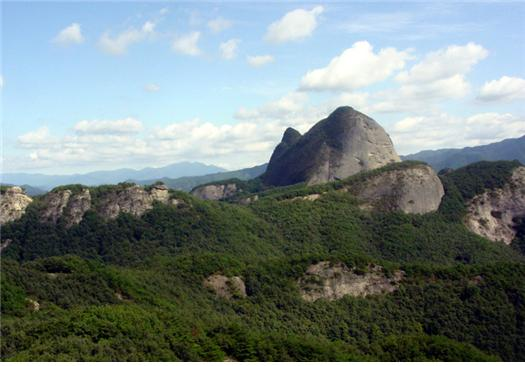
\includegraphics[width=0.8\textwidth]{./fig/SedimentaryRock_0001.jpg}
				\end{figure}

				마이산의 바위들은 운반작용을 통하여 퇴적된 퇴적암을 쇄설퇴적암이라 하는데, 이 쇄설퇴적암중 입자가 2mm 이상의 크기를 갖는 우세한 암석을 역암이라 한다. 
				마이산은 모두 역암이다. 
				마치 자갈과 시멘트를 섞어서 굳힌 것 같은 느낌이다.
				
				
				
			\paragraph{5) 각력암 [角礫岩, breccia]  }
				
				암석편이 퇴적될 때 그 모가 닳지 않고 거의 그대로 퇴적된 암석을 말한다.
				
				암석편이 원마작용(圓磨作用)을 받기 전에 퇴적한 퇴적암을 말한다. 각력암은 일반적으로 입경(粒徑)이 고르지 않고 크며, 여러 종류의 암석편이 섞여 있는 것이 보통이다. 
				단층각력으로 이루어진 단층각력암, 화산성인 응회각력암·화산각력암 등이 있다. 
				또 퇴적시 해저침식에 의해 생긴 셰일, 수중에 있던 이층(泥層)이 물이 마르면서 파쇄된 이암(泥岩), 산호초가 파도에 의해 파쇄되고 그 측면에 암석편이 퇴적하여 생긴 것 등은 모두 층내(層內) 각력암이다. 
				이밖에 애추(崖錐) 퇴적물이나 빙성(氷成) 퇴적물 등에서도 각력암을 볼 수 있다.
				


				\begin{figure}[h]
				\centering
				\caption{화산 각력암}
				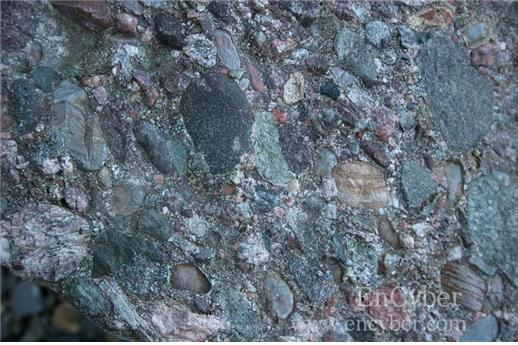
\includegraphics[width=0.8\textwidth]{./fig/SedimentaryRock_0002.jpg}
				\end{figure}

				\begin{figure}[h]
				\centering
				\caption{화산 각력암}
				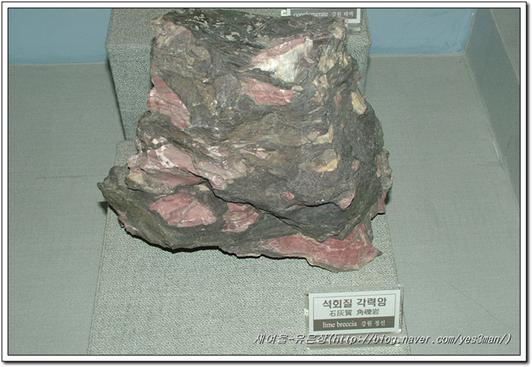
\includegraphics[width=0.8\textwidth]{./fig/SedimentaryRock_0003.jpg}
				\end{figure}


				\begin{figure}[h]
				\centering
				\caption{화산 각력암}
				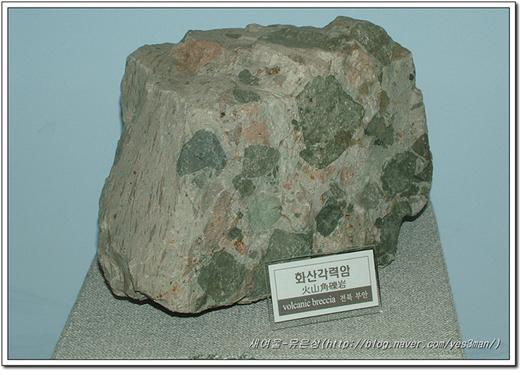
\includegraphics[width=0.8\textwidth]{./fig/SedimentaryRock_0004.jpg}
				\end{figure}



				
	\clearpage
%	----------------------------------------------------------------------------------------------------------------------- section
	\section{화학적 퇴적물}

			\begin{itemize}[	topsep=0.0em, itemsep=0.0em, leftmargin=4em, labelsep=3em ] 
			\item	모암이 풍화작용에 의하였거나 모암에서 분리된 암설로부터 수용성의 물질이 용해되어 일단 용액상태로 존재하는 것이 화학적 퇴적물이다.
			\item	이 퇴적물은 바다나 호수 등의 침전 장소로 이동하여 과포화가 일어난 곳에 침전되어 고화작용이 일어난다.
			\item	침전은 염분의 추가 및 증발로 물의 염분 농도가 커지거나 수온이 변할 때에 일어나며, 
					넓은 바다보다 폐쇄된 바다나 호수에서 침전이 빨리 일어난다.
			\end{itemize}	

		\paragraph{수용성의 물질}
			
		







	\clearpage
%	----------------------------------------------------------------------------------------------------------------------- section
	\section{유기적 퇴직물}

		유기적 퇴적물은 생물의 유해가 쌓여서 만들어진 퇴적물이다.
		동물은 주로 그 껍질이나 뼈를 퇴적물로 공급하는데 그 성분은 물에 용해되어 있던 무기물로서 이들은 생물화학적인 퇴적물이라고 할 수 있다.
		식물은 $CO_2$로 부터 취한 탄소를 포함한 유해를 퇴적하여 탄소를 주성분으로 하는 퇴적암, 즉 석탄을 만드는 경우가 있다.







	\clearpage
%	----------------------------------------------------------------------------------------------------------------------- section
	\section{속성 작용}






		\paragraph{이산화 규소$SiO_2$}





% 	======================================================================================================================= chapter
	\clearpage
	\chapter{퇴적암의 특성}
	\minitoc				% Creating an actual minitoc



	\clearpage
%	----------------------------------------------------------------------------------------------------------------------- section
	\section{퇴적암의 특성}


		퇴적암은 퇴적물이 바다나 호수 및 강바닥과 같은 물 밑이나 육지의 어느 한 곳에 쌓여서 만들어진 것이므로 화성암과는 구별이 가능한 몇가지 특징을 가진다.
		그 중 대부분의 퇴적암이 가진 특징으로 중요한 것은 층상으로 발달되는 평행구조로서 이것이 층리(bedding)이다. 
		이 밖에 결핵체, 사층리, 물결자국, 건열, 빗자국 등과 화석이 포함된다.
		이들은 퇴적암에서만 볼 수 있는 특징이다.



	\clearpage
%	----------------------------------------------------------------------------------------------------------------------- section
	\section{층리}



		퇴적물이 쌓이는 바다 밑바닥은 대체로 수평인 면이며 이 면 위에 퇴적물이 거의 고르게 한 겹 한 겹 쌓여서 점점 두꺼운 지층이 형성된다.
		이 층과 층 사이의 면은 퇴적물이 굳어진 후에도 잘 쪼개지는 면을 형성하며 이 면을 층리면(bedding plane)이라고 한다.

		\paragraph{엽층}
			층리들 중 두께가 1 cm 이하의 얇은 층리를 엽층(lamina)이라 한다.

		\paragraph{괴상 퇴적암}
			1 m 이상 두꺼운 층리를 가지는 퇴적암을 괴상(massive)의 퇴적암이라고 부른다.


		\paragraph{생란 작용 : 층리의 생물에 의한 교란  }
			때로는 퇴적물에 잘 발달된 층리가 생물에 의해 교란되어 층리가 없어지는 경우가 있다.
		생물의 이러한 교란작용을 생란작용(bioturbation)이라고 하며 생란작용이 심하면 퇴적물을 잘 혼합시켜 균일하게 하기도 한다.

		\paragraph{층리의 절리와의 혼동}
			어떤 암석에는 절리가 잘 발달되어 마치 층리와 같아 보이는 일이 있다.
			이런 경우에는 층리에 따른 입자들의 배열 상태에 주의하여 관찰하여 절리와 층리와의 혼동을 피하도록 한다.


		\paragraph{층리의 성인}
			층리의 성인은 시간을 달리하여 순차로 쌓이는 퇴적물의 입자의 크기, 퇴적물의 종류와 색, 운반 매질 등의 변화 때문이다.
			이러한 변화를 일으키는 원인을 보면 다음과 같다.

일기, 계절 및 기후의 변화 :
해저의 심도 변화 :
해류의 변화 :
해수와 호수 농도 및 수온의 변화 :
생물의 성쇠  : 식물 또는 동물이 상기한 환경 변화와 진화에 의한 변화로 번성 또는 쇠퇴할 때 그 유해의 공급이 가감되어 층리가 생성된다.


























	\clearpage
%	----------------------------------------------------------------------------------------------------------------------- section
	\section{사층리}



		\paragraph{사층리의 형성}
		모래가 쌓여 형성된 사암층에는 층리가 일정한 방향을 가지지 않는 경우가 가끔 관찰된다.
		이런 복잡한 층리를 사층리라고 하는데, 이는 모래를 운반한 바람이나 물이 한 방향으로만 움직이지 않는곳에 쌓인 지층임을 표시한다.
		즉 수심이 대단히 얕은 물 바닥이나 사막의 사구에서 볼 수 있는 퇴적구조이다.

		
		\paragraph{사층리의 각도}
		퇴적물이 쌓이며 사층리를 형성할 당시에는 사층리의 각도는 25도 $\sim$ 35도의 안식각을 유지하나 
		퇴적 후의 다짐작용으로 퇴적 당시보다는 휠씬 작은 각도(15도 $\sim$ 20도)를 가지게 된다.
		그러나 지층이 횡압력을 받아서 변형하게 되면 도리어 안식각보다 큰 각도를 보이는 경우도 있다.

		\paragraph{사층리를 통한 퇴적의 순서}
		어는 경우든 사층리가 있으면 퇴적의 순서를 쉽게 알아 낼 수 있다.
		만일 지층이 지작변동으로 뒤집혀 있으면 그 사실을 곧 판단할 수 있으므로 지질학상 중요한 자료가 된다.
		또한 지층에 나타난 사층리를 많이 측정하여 그 방향을 통계적으로 처리하면 
		그 지층이 퇴적할 때의 고수류의 방향과 퇴적물의 공급원을 알 수 있는 주요한 구조이다.


		\paragraph{경상분지의 사층리}
		우리나라 남동부의 경상분지에서는 사층리의 분석을 이용하여 
		중생대 백악기의 퇴적암들이 퇴적 당시 대체로 북서쪽에서 남동쪽으로 물이 흘렀음이 밝혀져 있다.







	\clearpage
%	----------------------------------------------------------------------------------------------------------------------- section
	\section{물결자국(연흔)}


			\begin{itemize}[	topsep=0.0em, itemsep=0.0em, leftmargin=4em, labelsep=3em ] 
			\item	잔물결이나 물결의 흐름이 그 아래 얕게 쌓인 퇴적물의 표면에 미치면 퇴적물의 표면에 파상의 요철, 즉 물결 자국이 새겨진다.
			\item	이것이 퇴적작용이 계속되는 동안에도 파괴되지 않고 있으면 층리면 상에 그대로 보존되어 나타난다.
			\item	경상남북도의 중생대층 퇴적암 중에서 특히 자주 발견된다.
			\item	물결자국에는 정부가 뾰쪽하고 곡부가 평탄한것이 있으며 이런 물결자국을 포함하는 지층은 
					변형작용을 받아 지층이 역전될 경우에도 그 퇴적 순서를 판단하는데 이용된다.
			\item	수심이 깊은 바다나 호수에서 퇴적된 퇴적암에서는 물결자국이 생기기 어려우며, 
					물결자국은  사층리와 함께 퇴적 환경을 연구하는데 중요한 자료가 된다.
			\end{itemize}	







	\clearpage
%	----------------------------------------------------------------------------------------------------------------------- section
	\section{건열}


			\begin{itemize}[	topsep=0.0em, itemsep=0.0em, leftmargin=4em, labelsep=3em ] 
			\item	얕은 물 아래에 쌓인 점토 성분의 퇴적물이 한때 수면 위에 노출되어 건조하게 되면 
					수분의 증발로 퇴적물의 표면이 수축하여 틈이 생긴다.
			\item	이러한 틈을 건열이라고 한다.
			\item	건열이 파괴되지 않고 묻혀서 지층 중에 보존되는 일이 많다.
			\item	건열은 밑으로 향하여 쐐기 모양의 단면을 보여 준다.
			\item	건열구조가 발달하는 지층에서는 지층의 상하판단의 기준이 되기도 한다.
			\end{itemize}	









	\clearpage
%	----------------------------------------------------------------------------------------------------------------------- section
	\section{결핵체}

			\begin{itemize}[	topsep=0.0em, itemsep=0.0em, leftmargin=4em, labelsep=3em ] 
			\item	퇴적암 중에는 자갈모양의 구형이나 반구형 혹은 불규칙한 모양을 가진 단단한 물체가 
					마치 퇴적암 내에 마치 자갈처럼 들어 있는 경우가 관찰되는데 이들을 결핵체라고 한다.
			\item	그 직경은 수 mm에서 수 m에 달하는 것까지 있다.
			\item	그 성분은 인산염, 경석고, 방해석, 규산, 갈철석, 적철석, 능철석 혹은 황철석이 보통이며, 
					이들이 수중에 용해되어 있다가 어떤 입자를 중심으로 침전을 일으키면서 서로 뭉쳐서 만들어진 것이다.
			\item	성인적으로는 두 종류가 존재할 수 있으며, 
					하나는 퇴적물이 쌓일 때에 동시적으로 물밑에서 성장하다가 퇴적물로 덮인 것이고, 
					다른 하나는 퇴적암이 생성된 후에 지층 중의 어떤 입자가 핵이 되어 지하수에 녹아 있는 광물질을 집결시킨 것이다.
			\end{itemize}	








	\clearpage
%	----------------------------------------------------------------------------------------------------------------------- section
	\section{화석}


		\paragraph{화석}
		퇴적물이 침전되던 당시에 수중에 살던 생물의 유해가 지층과 같이 쌓여서 지층 중에 남아 있으면 이들의 화석이라고 한다.

		\paragraph{생흔 화석}
		이밖에도 생물의 유해는 아니지만 퇴적암 속에 생물체의 흔적으로 생물체가 만든 구멍, 발자국, 기어간 자국 등이 남아 있는 경우가 있으며, 
		이들을 통틀어서 생흔화석(trace fossils)이라고 한다.
		생흔화석은 퇴적 속도, 퇴적 양상, 퇴적 환경, 고생물의 생태 등에 관한 여러 가지 지질학적 정보를 제공한다.






% 	======================================================================================================================= chapter
	\clearpage
	\chapter{퇴적암의 특성 2}
	\minitoc				% Creating an actual minitoc




	\clearpage
%	----------------------------------------------------------------------------------------------------------------------- section
	\section{퇴적암의 특성}


		
		\subsection{퇴적암의 분류 및 특성}

			\subsubsection{쇄설성 퇴적암}
		%		\tabulinesep=0.6ex
				\begin{tabu} to 1.0\textwidth { X[l, 2.0] X[l, 4.0] X[l, 4.0] X[l, 4.0] X[l, 4.0]}
				\tabucline[0.2ex]{-}		
				암종		&구성 물질		&입 경(mm)		&조성				&퇴적 환경 	\\
				\tabucline[0.1ex]{-}		
				역암		&표력			&>256			&모암과 동일			&하천바닥 기반암에는 잘 나타나지 않음\\
						&왕자갈			&256~64			&모암과 동일			&하천바닥 충적선 상지 하천유로에 퇴적	\\
						&잔자갈			&64~4			&왕자갈 모래와 동일		&왕자갈과 동일 해변에도 퇴적		\\
						&왕모래			&4~2			&왕자갈 모래와 동일		&잔자갈이나 모래와 동일	\\
				사암		&모래			&2~0.02			&석영이 가장우세, 장석, 석류석,  마그네타이트로 구성 부분적으로 각섬석, 휘석, 조개조각 포함
																		&충적퇴적층 하천유로, 선상지, 범람원, 해안, 삼각주에 퇴적 간혹 풍성퇴적 \\
				실트스톤	&실트			&0.02~0.002		&모래와 동일 간혹 점토포함	
																		&삼각주 범람원	\\
				셰일		&점토			&<0.002			&불안정광물이 변질되어 최종적으로 형성 함수규산염생성 \\
						&				&				&					&정수, 해수 : 점토가 덩어리로 되어 신속하게 바닥에 침전, 층리가 발달하지 않음. \\
						&				&				&					&담수 : 천천히 침전, 층리가 발달 \\
				\tabucline[0.1ex]{-}		
				\end{tabu} 

			\subsubsection{비쇄설성퇴적암(화학적, 유기적 퇴적암)}
		%		\tabulinesep=0.6ex
				\begin{tabu} to 1.0\textwidth { X[l, 2.0] X[l, 4.0] X[l, 4.0] X[l, 4.0] X[l, 4.0]}
				\tabucline[0.2ex]{-}		
				암종		&구성 물질		&입 경(mm)		&조성				&퇴적 환경 	\\
				\tabucline[0.1ex]{-}		

				석회암	&석회질 침전물		&				&괴상 방해석			&심해, 정수상태 \\
				패각암	&석회질 침전물		&				&고결된 조개류			&해변, 온수	\\
				백악		&석회질 침전물		&				&유기물 잔재			&천재, 정수상태, 온수 \\
				백운암	&석회질 침전물		&				&백운암 - CaMg(CO3)2	&해수 침전 또는 석회암 교대작용 \\
				석고		&석회질 침전물		&				&석 고 - CaSO4․2H2O	&염수	\\
				쇄설성 퇴적물\\
				경석고	&석회질 침전물		&				&경석고 - CaSO4		&염수\\
				암염		&염분 침전물		&				&염화나트륨			&염수 \\
				석탄		&유기물			&				&탄산염				&늪지\\
				규질암	&규산염			&				&규산오팔				&침전 \\
				
				
				\tabucline[0.1ex]{-}		
				\end{tabu} 

			\subsubsection{쇄설성 퇴적물}
		%		\tabulinesep=0.6ex
				\begin{tabu} to 1.0\textwidth { X[l, 2.0] X[l, 4.0] X[l, 4.0] X[l, 4.0] X[l, 4.0]}
				\tabucline[0.2ex]{-}		
				암종		&구성 물질		&입 경(mm)		&조성				&퇴적 환경 	\\
				\tabucline[0.1ex]{-}		

				경석고	&석회질 침전물		&				&경석고 - CaSO4		&염수\\
				암염		&염분 침전물		&				&염화나트륨			&염수 \\
				석탄		&유기물			&				&탄산염				&늪지\\
				규질암	&규산염			&				&규산오팔				&침전 \\
				
				
				\tabucline[0.1ex]{-}		
				\end{tabu} 



	\clearpage
%	----------------------------------------------------------------------------------------------------------------------- section
	\section{쇄설성 퇴적암의 특징}


		\paragraph{1. 조 립 질(직경 2mm 이상)}

			\begin{itemize}[topsep=0.0em, parsep=0.0em, itemsep=0em, leftmargin=10.0em, labelwidth=3em, labelsep=3em] 
			\item [역암 일반] 	암종에 관계없이 원마도 양호. 석영성분 우세.\\
							고결물질은 주로 규산염이지만 간혹 산화철, 점토, 석회질 물질인 경우도 있음 
			\item [역암]		세립질 바탕에 굵은 입자가 발달
			\item [기저역암]	층중에 제일 처음나타나는 층. 부정합면 형성
			\item [각력암]		암종에 관계없이 각진 암편. 빙하작용, 낙석, 공동붕괴, 단층작용에 의해 형성
			\end{itemize}


		\paragraph{2. 중 립 질(입경 0.02~2mm 50\%이상)}

			\begin{itemize}[topsep=0.0em, parsep=0.0em, itemsep=0em, leftmargin=10.0em, labelwidth=3em, labelsep=3em] 
			\item [사암]		주로 규산염이나 산화철, 점토, 방해석과 같은 탄산염으로 고결된 석영성분으로 구성.\\
							고결물질에 의해 암색 결정. 산화철이 우세할 경우 황색, 갈색, 적색을 띠며 규산염이나 석회질이 우세할 경우 담색을 띰.  \\
							투수성 암석으로 간극률이 5~30\%이상임. \\
							암층이 비교적 단단하고 층후가 두꺼움.
			\item [야코스사암]	사암과 비슷하나 장석이 최소한 25\% 이상임.
			\item [경사암]		점토 바탕에 석영과 장석이 우세하게 나타나며 비교적 각진 다른 광물이 다양하게 존재
			\end{itemize}
			
			
		\paragraph{3. 세립질}

			\begin{itemize}[topsep=0.0em, parsep=0.0em, itemsep=0em, leftmargin=10.0em, labelwidth=3em, labelsep=3em] 
			\item [실트스톤] 	구성이 사암과 비슷하나 50\% 이상되는 입자의 입경이 0.002~0.02mm 임.
							층후가 비교적 두꺼우며 단단함.
			\item [셰 일 일반] 입경이 대부분 0.002mm(콜로이드) 이하임. 잘 갈라짐. 산화철이 포함되면 적색을 띠   고 탄산염이 포함되면 회색 내지 흑색을 띰. 일반적으로 사암과 호층을 이루는 경우   가 많고 비교적 연약함. 비교적 변종이 많음.
			\item [아질라이트] 단단하게 굳은 셰일이나 셰일보다 덜 갈라짐. 점판암과 유사하나 점판암에 발달하는   벽개는 발달하지 않음. 
			\item [석회질셰일] 방해석과 같은 탄산염 포함. 석회질 성분이 증가하면 셰일질 석회암으로 분류
			\item [탄질셰일]	흑색셰일은 탄소와 같은 유기물질을 많이 포함하고 있기 때문에 탄층으로 변화하는   경우가 많이 있음.
			\item [오일셰일]	탄산염 성분이 포함되며 이 부분이 파괴되어 증류되면 석유 형성
			\item [해성셰일]	일반적으로 포화시나 건조시에 부피변화가 매우 큰 팽창성점토(몬모릴로나이트)가 포   함되어 있음. 
			\item [점토질셰일]	중간정도 굳은 단단한 셰일
			\item [이암]		점토크기의 입자들이 암석에 가까울 정도로 다져져 있으나 균열이 발생하지는 않음.   지질적인 관점에서는 단단한 점토를 의미하기도 함.
			\end{itemize}

	\clearpage
%	----------------------------------------------------------------------------------------------------------------------- section
	\section{비쇄설성 퇴적암의 특징}
		

		\paragraph{1. 석회질 침전물}

			\begin{itemize}[topsep=0.0em, parsep=0.0em, itemsep=0em, leftmargin=10.0em, labelwidth=3em, labelsep=3em] 
			\item [석회암 일반]	암종에 관계없이 원마도 양호. 석영성분 우세. 고결물질은 주로 규산염이지만 간혹    산화철, 점토, 석회질 물질인 경우도 있음 
			\item [결정질 석회암]	세립질 바탕에 굵은 입자가 발달
			\item [micrite] 		층중에 제일 처음나타나는 층. 부정합면 형성
			\item [어란상 석회암]	암종에 관계없이 각진 암편. 빙하작용, 낙석, 공동붕괴, 단층작용에 의해 형성
			\item [화석질 석회암]	연체동물이나 바다나리 같은 무척추동물이나 탄산칼슘으로 고결된 산호와 같은 유기   물로 이루어짐. 
			\item [패각암]			조개나 조개파편이 약하게 고결되어 형성한 간극률이 높은 암석. 남대서양 쪽 미국   해안이나 바하마군도를 따라 많이 분포
			\item [백악]			간극률이 높고 약하며 세립질임. 조개나 극소형의 유기물로 구성 일반적으로 백색을   띠며 백악기층에 널리 분포.
			\item [백운암]			석회암보다 단단하고 무거움 (단위중량 : 석회암 2.71㎏/㎤, 백운암 2.87㎏/㎤)
								해수에서 직접 침전되어 형성되거나 석회암의 교대작용으로 백운암화되어 형성. 분   말로 만들 경우 염산과 반응하여 거품형성. 경도 5이상
			\item [석고]	 		증발잔류암으로 괴상구조를 나타냄. 백색이고 약함.
			\item [강석고]			 증발잔류암. 약하기는 하나 석고보다는 강함. 경석고 입자로 이루어짐. 은미장질 내   지는 현정질. 일반적으로 찢어진 조각같은 구조를 나타내며 백색에 진주광택을 보임.
			\item [암염]			증발잔류암. 결정질 소금입자가 모여 형성. 약하고 저온저압 상태에서 유동하는 성질을 보임. 
								암염돔을 형성함. 
								주변 암반에 비중이 훨씬 작기 때문에 상부암반이 침식되면 지표로 솟아올라와 돔형의 지각변형 발생. \\
								주변 암반도 변형이 일어나며 암염으로 이루어진 암주가 상승함에 따라 균열발생. \\
								이 과정에서 원유를 가두어 둘 수 있   는 지질구조 형성
			\end{itemize}
 
		\paragraph{2. 탄질물질로 이루어진 유기질 퇴적암}
			\begin{itemize}[topsep=0.0em, parsep=0.0em, itemsep=0em, leftmargin=10.0em, labelwidth=3em, labelsep=3em] 
			\item [석탄]			심하게 변질된 식물잔유물과 점토로 이루어지며 흑색내지 갈색을 띰. 온도와 압력에   따라 이탄이 탄화하는 정도가 다름. 갈탄이 역청질 석탄으로 변하며 최종적으로 무   연탄으로 변함
			\end{itemize}

		\paragraph{3. 생화학적 기원의 규질 퇴적암}
			\begin{itemize}[topsep=0.0em, parsep=0.0em, itemsep=0em, leftmargin=10.0em, labelwidth=3em, labelsep=3em] 
			\item [규질암]			증발이나 수중에 생존하는 유기물의 작용으로 규산이 퇴적하여 형성. 화학반응에 의   해서도 형성. 
								소규모 결핵체로 산출되거나 넓은 지역에 걸쳐 두꺼운 퇴적층 형성. 
								석회암층이나 백악층에 잘 발달. 경도가 7이며 이로 인해 석회암이 풍화로 제거되어도   규질암은 변화되지 않은 채 그대로 남아 있으며 적색 또는 적갈색 규질암을 특히 벽옥이라함 .
			\item [규조암]			약하고 백색을 띠며 백악과 유사함. 아주 작은 규조 껍질로 이루어져 매우 가벼움.    간극률이 높음. 
			\end{itemize}



	\clearpage
%	----------------------------------------------------------------------------------------------------------------------- section
	\section{퇴적암의 공학적 특성 : 1. 일반적인 공학적 특성}


			
				\tabulinesep=0.6ex
				\begin{tabu} to 1.0\textwidth { X[l, 2.0] X[l, 4.0] X[l, 3.0] X[l, 4.0] X[l, 3.0]}
				\tabucline[0.2ex]{-}		
				암종			&특성								&투수계수			&변형정도							&강도				\\
				\tabucline[0.1ex]{-}	
				사암			&간극이 고결물질로 채워짐				&낮음			&낮음							&높음				\\
							&고결물질이 간극을 부분적으로 충진			&매우높음			&중간 - 높음						&중간 - 낮음				\\
				\tabucline[0.1ex]{-}		
				셰일			&암석화 정도에 따라 다름					&불투수성			&높음 - 낮음						&낮음 - 높음				\\
							&									&				&팽창성이 높을 수 있음				&				\\
				\tabucline[0.1ex]{-}		
				석회암		&순수할수록 공동 발달					&공동주변이 높음	&동굴 아치부를 제외하고는 낮음.		&동굴 아치부를 제외하고는 높음.				\\
							&불순물								&불투수성			&일반적으로 낮음.					&일반적으로 높음				\\
				\tabucline[0.1ex]{-}		
				백운암		&공동이 거의 발달하지 않음				&불투수성			&석회암보다 낮음.					&석회암보다 높음				\\ 
				\tabucline[0.1ex]{-}		
				\end{tabu} 




	\clearpage
%	----------------------------------------------------------------------------------------------------------------------- section
	\section{퇴적암의 공학적 특성 :  2. 암종에 따른 일축압축강도, 단위중량, 변형계수}  


		%		\tabulinesep=0.6ex
				\begin{tabu} to 1.0\textwidth { X[l, 2.0] X[l, 2.0] X[l, 2.0] X[l, 2.0] X[l, 2.0] X[l, 2.0] }
				\tabucline[0.2ex]{-}		
				\tabucline[0.1ex]{-}		
				
				암종		&구조			&조직			&γd, 			&Uc,				&Er		\\
						&				&				&g/㎤			&㎏/㎠			&㎏/㎠		\\
				\tabucline[0.1ex]{-}		
				\tabucline[0.1ex]{-}		
				
				역암		&조립-원형		&층상, 고결		&2.48			&350~1050		&7~35		\\
				각력암	&조립-각형		&층상, 고결		&2.53			&350~1050		&7~35		\\
				사암		&중립			&층상, 고결		&2.35			&280~840			&7~21		\\
				이암		&세립			&층상, 고결		&1.8~2.4			&7~350			&3~14		\\
				셰일		&매우세립			&박편상, 다져진 셰일- 불안정	고결된 셰일 - 안정
														&1.6~2.2			&7~350			&3~14		\\
				석회암	&세립			&괴상, 층상, 용해성, 용해공동
														&2.64			&350~1050		&14~42		\\
				백운암	&세립			&괴상 간혹 재결정	&2.67			&490~1400		&28~56		\\
				\tabucline[0.1ex]{-}		
				\end{tabu} 




			

% 	======================================================================================================================= chapter
	\clearpage
	\chapter{퇴적암류}
	\minitoc				% Creating an actual minitoc
	


	\clearpage
%	----------------------------------------------------------------------------------------------------------------------- section
	\section{퇴적암류}

				퇴적암류는 국토의 약 20\%를 덮고 있다. 
				고생대 이전에 쌓인 퇴적암류는 모두 변성암류로 변질되었다. 

			\paragraph{(1) 조선누층군}
			고생대 초에 평안 분지에서 해성층으로 쌓인 조선누층군(組鮮累層群)은 평남과 황해도에 가장 넓게 분포하며, 
			남한에서는 옥천지향사에 속한 강원도 남동부와 이에 인접한 충북, 경북의 일부 지역에도 넓게 나타난다. 
			조선누층군은 대부분 석회암으로 이루어졌다. 
			이 석회암은 시멘트의 원료로 쓰이며, 삼척·동해·영월·단양·문경 등지의 시멘트공업은 이를 바탕으로 발달했다. 
			석회암의 분포 지역에서는 석회 동굴·돌리네·라피에와 같은 카르스트 지형이 형성되어 있다. 


			\paragraph{(2) 개결층}
			조선누층군이 퇴적된 이후 한반도는 융기하여 석탄기 초에 이르기까지 오랫동안 육지로 남아 있어서 지층이 쌓이지 않았다. 
			이 기간을 지질학에서는 대결층(大缺層)이라고 부른다. 


			\paragraph{(3) 평안누층군}

			대결층 다음 고생대 말∼중생대 초에 걸쳐 퇴적된 평안누층군(平安累層群)은 조선누층군과 거의 같은 지역에 분포하나 그 면적이 보다 협소하다. 
			주요분포지역은 평남 북부와 평양 부근, 황해도 남동부, 강원도 남동부, 충북 북동부, 전남 중부 등이다. 
			평안누층군은 육성층으로 이루어졌으며, 평양 탄전을 위시하여 삼척·영월·정선·단양·문경 등지의 탄전에 매장된 무연탄을 포함하고 있다. 
			전남 화순 탄전의 무연탄도 평안누층군에 속한 것이다. 
			그런데 평안누층군은 송림변동(松林變動)에 의한 습곡·단층작용을 받아 심하게 교란되었으며, 따라서 무연탄의 부존상태가 연속적이지 않다. 



			\paragraph{(3) 대동누층군}
			중생대의 지층은 대동누층군(大同累層群)과 경상누층군으로 나뉜다. 
			중생대 중기의 대동누층군은 평안누층군이 퇴적된 다음 
			넓은 지역이 육지로 변함에 따라 생긴 소규모의 호분(湖盆 분지 안의 호수?)에 쌓인 육성층으로서 
			충남의 보령을 중심으로 그 주변의 서천·부여를 포함한 지역에 주로 분포한다. 
			충남 탄전의 무연탄은 대동 누층군에 매장되어 있다. 
			대동누층군이 쌓인 후에는 한반도의 지사(地史)에서 가장 격렬했던 대보조산운동(大寶造山運動)이 일어나서 지층의 교란이 더욱 심해졌다. 


			\paragraph{(4) 경상누층군}
			경상누층군(慶尙累層群)은 백악기에 형성되었고, 이의 퇴적 장소가 경상남·북도에 걸친 경상분지이다. 
			경상누층군은 경상남·북도 이외에 전북의 동부 산간 지방, 충북의 영동·진천 등지에도 소규모로 분포한다. 
			경상누층군의 하부층은 역암·사암·셰일 등으로 이루어졌고, 
			상부층은 위로 올라갈수록 화산 활동에 의한 안산암·유문암·응회암 등의 화산암이 늘어나다가 
			결국 퇴적암은 그 사이에 끼어 있는 상태로 나타난다.  
			이러한 암석은 퇴적암으로 보기가 어려워서 과거에는 화산암으로 분류했었으나 지금은 경상누층군의 '유천층군'에 포함시키고 있다.  \\


			백악기 말에는 한반도 남부에서 화산 활동이 격심하게 일어났다. 
			유천층군(楡川層群)의 화산암류는 호남지방에도 널리 분포한다.
			청송의 주왕산, 의성의 금성산, 정읍의 내장산, 고창의 선운산, 목포의 유달산 등은 백악기의 화산암류로 이루어졌다.
			광주의 무등산에서는 안산암의 주상 절리에 의한 지형(立石臺·瑞石臺)도 볼 수 있다.
 
			백악기 말에서 신생대 제3기초에 걸쳐 일어난 불국사 변동(佛國寺變動)은 습곡 작용을 경미하게 수반했다. 
			그래서 지층이 기울어지기는 했으나 대구 부근의 경부 고속도로 연변에서 보이는 바와 같이 원래의 수평 구조를 보존하고 있는 것이 보통이다. 

			신생대 제 3기층은 포항 분지와 두만 분지에 비교적 넓게 나타난다. 함북의 아오지·명천 등지의 제3기층에서는 갈탄이 산출된다. 





% 	======================================================================================================================= chapter
	\clearpage
	\chapter{퇴적암의 분류}
	\minitoc				% Creating an actual minitoc
	


	\clearpage
%	----------------------------------------------------------------------------------------------------------------------- section
	\section{퇴적암의 분류}


		퇴적암은 퇴적물들이 강이나 바다 혹은 호수 등지나 풍력에 의해 쌓여서 된 암석이다.
		그러니만큼 퇴적물의 크기 즉 구성물질의 입자크기가 퇴적암을 명명하는데 첫 번째 기준이 된다.

		또한 퇴적물의 종류에 따라 쇄설성 퇴적물에서 유래된 쇄설성 퇴적암과 
		그 외 화학적 내지 유기적 퇴적물에서 유래된 비쇄설성 퇴적암이 그 분류기준이다.




	\clearpage
%	----------------------------------------------------------------------------------------------------------------------- section
	\section{퇴적암의 종류}
	
	
				
		\subsection{쇄설성 퇴적암}


			\paragraph{1) 해성,유성 쇄설암}
				주로 유수에 의하여 운반, 퇴적 \\

				쇄설성 퇴적암은 암석을 구성하는 입자의 크기에 따라 역암에서 이암까지 분류되며 
				자갈과 같이 비교적 입자가 큰 퇴적물이 운반되고 쌓여서 암석화가 된 것을 \textbf{역암}이라 하며,
				반대로 입자가 매우 적은 펄 등이 암석화가 된 것을 \textbf{이암} 혹은 \textbf{셰일}이라 하며, 
				모래가 암석이 된 것을 \textbf{사암}이라 한다.

				\begin{itemize}[topsep=0.0em, parsep=0.0em, itemsep=0em, leftmargin=6.0em, labelwidth=3em, labelsep=3em] 
				\item [역암]	퇴적암의 한 가지. 자갈이 해안 $\cdot$ 물바닥에 퇴적하여 석회질 $\cdot$ 점토질 또는 규질의 응결 물질에 의하여 굳어진 것. 
							특히 둥글지 아니한 것을 각력암(角礫岩)이라 함. 자갈돌 
				\item [사암]  	모래가 뭉쳐서 단단히 굳어진 암석. 흔히 모래에 점토가 섞여 이루어지는데 건축 재료나 숫돌로 쓴다.
				\item [이암]  	미세한 진흙이 쌓여서 딱딱하게 굳어 이루어진 암석. 뻘돌 $\cdot$ 진흙 바위.
				\item [셰일] 	점토가 굳어져 이루어진 수성암(水成巖). 회색이나 검은 갈색을 띠며, 흔히 얇은 층(層)으로 되어 잘 벗겨지는 성질이 있다. 
							이판암 $\cdot$ 혈암(血巖).
				\end{itemize}
		

			\paragraph{2) 화산쇄설암} \tab \tab
					화산 쇄설암은 화산활동과 수반하여 발생한 쇄설물들이 공중으로 분출하였다가 중력에 의해 지표에 쌓인 것으로 
					쇄설물의 크기에 따라 화산 각력암에서 화산재로 이루어진 응회암까지 분류 된다.

					화산 분출물이 쌓여 굳으면서 이루어진 암석을 통틀어 이르는 말. 화산력, 각력암, 응회암 따위로 나눈다. 
					[비슷한 말] 화성 쇄설암 $\cdot$ 화쇄암.

				\begin{itemize}[topsep=0.0em, parsep=0.0em, itemsep=0em, leftmargin=6.0em, labelwidth=3em, labelsep=3em] 
				\item [화산력]
				\item [각력암]
				\item [응회암]
				\end{itemize}

		\subsection{비쇄설성 퇴적암}

			\paragraph{1) 유기적 퇴적암 (생물 유해의 집합)} 

			\paragraph{2) 화학적 퇴적암 (화학적 침전물의 집합)}


	
	
	
	
	
	
	
	
	
	
	
	
	
	
	
	
	
	
	
	
	
	
	
	
	
	
	
	
	
	
	
	\clearpage
%	----------------------------------------------------------------------------------------------------------------------- section
	\section{셰일  shale }


		\subsection{셰일 shale}
		
			퇴적암 중 특히 얇은 엽층리가 발달하며 이 면을 따라 판상의 쪼개짐이 있으면 셰일이라 한다.

				\begin{figure}[h]
				\centering
				\caption{화산 각력암}
				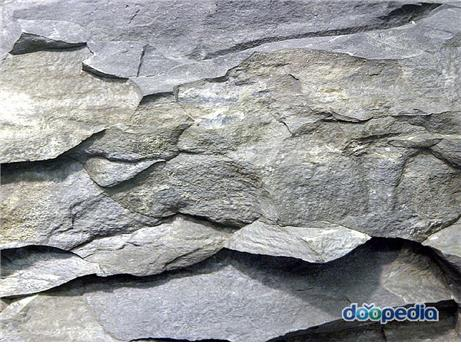
\includegraphics[width=0.8\textwidth]{./fig/shale_0001.jpg}
				\end{figure}

		\clearpage  \vskip  4em
		\subsection{셰일}

			운반작용으로 생성되는 퇴적암 중 입자의 크기가 63㎛(마이크로미터)보다 작고, 층과 평행하게 벗겨지는 암석.

			입자의 크기가 63㎛보다 작은 세립질의 암석으로, 전형적 층상구조를 보여 쪼개짐이 나타난다. 

			성층면(成層面)을 따라 평행하게 얇은 층으로 쪼개지는 성질을 가지는데, 이것은 입자의 크기가 다르거나 구성광물의 색이 다를 경우 나타난다. 
			흰 쌀과 검은 쌀을 층층이 쌓은 것을 생각하면 된다. 
			붉은색, 녹색, 검은색, 회색 등 여러 색이 나타난다.\\
			
			[네이버 지식백과] 셰일 [shale] (두산백과)



		


		\clearpage  \vskip  4em
		\subsection{적색 셰일}

				1/16 크기 이하의 진흙 입자들이 쌓여 굳은 암석, 결을 따라 쉽게 벗겨지며 지각의 70\%를 구성한다.

	
	
	
	
	\clearpage
%	----------------------------------------------------------------------------------------------------------------------- section
	\section{이판암}
	
	
	
	\clearpage
%	----------------------------------------------------------------------------------------------------------------------- section
	\section{혈암}
	



	

	\clearpage
%	----------------------------------------------------------------------------------------------------------------------- section
	\section{이암}







	
	
	
	\clearpage
%	----------------------------------------------------------------------------------------------------------------------- section
	\section{사암}
	







	
	
	
	
	
	
% 	======================================================================================================================= chapter
	\clearpage
	\chapter{역암 礫巖 Conglomerate}
	\minitoc				% Creating an actual minitoc
	

	
	\clearpage
%	----------------------------------------------------------------------------------------------------------------------- section
	\section{역암 礫巖 Conglomerate}
	


		\subsection{요약}
				크기가 2mm 이상인 둥근 알갱이가 30\% 이상 들어 있는 쇄설성 퇴적암.



		\clearpage   \null \vskip 1em
		\subsection{역암}


				역암은 크기가 2mm 이상인 둥근 알갱이가 30\% 이상 들어 있는 쇄설성 퇴적암이다. 
				크기가 2~4mm의 퇴적 알갱이를 그래뉼(Granule), 4~64mm의 퇴적 알갱이를 자갈, 
				64~256mm의 퇴적 알갱이를 왕자갈, 256mm 이상의 알갱이를 거력(Boulder)이라고 하는데, 
				역암에는 크기가 2mm 이상인 알갱이들이 많이 들어 있는 것이다. 

				경우에 따라서 2mm 이상의 퇴적 알갱이가 10\%만 되어도 역암으로 분류하기도 하지만 
				일반적으로는 2mm 이상의 알갱이가 30\% 이하이면 역질사암, 역질석회암, 거력점토암 등으로 분류한다. 

				역암은 암석에 들어 있는 자갈이 둥근 모양이며, 각력암은 암석에 들어 있는 자갈이 각이 져 있는 모난 모양이다. 
				역암은 정역암과 준역암으로 분류되기도 하며, 
				정역암은 역지지역암이고, 준역암은 기질지지역암이다. 정역암을 역암, 준역암을 잡역암이라고도 한다. 
		
				정역암은 해변이나 하천 등 물의 흐름이 빨라 광물 알갱이의 크기가 5mm 이상으로 큰 조립질 퇴적 알갱이가 풍부한 곳에서 만들어지며, 
				준역암은 선상지가 만들어지는 곳처럼 물의 흐름이 갑자기 느려져서 빠르게 퇴적이 일어나는 곳에서 만들어진다. 
				그 결과 정역암은 '역'이라고도 하는 알갱이의 지름 2 mm 이상인 암석 파편들이 서로 접촉하고 있는 골격 구조가 나타나는 반면, 
				준역암은 역들이 서로 간에 접촉하지 않고 기질 내에 흩어져서 존재하는 구조를 갖게 되는 것이다. 

				정역암을 이루는 역들은 크기가 비슷하고 준역암을 이루는 역들은 크기가 다양하다. 
				역암을 구성하는 역들은 대체로 석영, 규암, 석영질사암, 처트 등과 같이 안정된 광물로 이루어져 있으므로, 
				역암은 잘 변하지 않고 내구성이 높은 암석이다. 

				우리 나라에서는 대부분의 퇴적 분지에서 역암이 산출된다. 
				삼척 태백 지역의 고생대 지층인 세송층에서는 석회질 역암이 산출되고, 
				중생대 백악기 지층인 진안 지역의 마이산의 역암층에서는 왕자갈, 거력질 역암이 산출된다. 
				또한, 경상남·북도 서부 지역에는 중생대 백악기의 지층인 경상 누층군 에서 긴 띠 모양으로 신라역암층이 분포되어 있다.



	\clearpage
%	----------------------------------------------------------------------------------------------------------------------- section
	\section{역암의 특징}


				역암을 관찰하면 자갈이 들어 있는 것을 볼 수 있다. 
				자갈은 지름이 2mm 이상인 알갱이이다. 
				자갈의 모양은 둥근 것도 있고 모난 것도 있으며, 자갈의 색도 흰색, 붉은색, 검은색 등 다양하다. 
				자갈이 들어 있는 모양도 달라서 자갈과 자갈이 서로 닿은 것도 있고, 자갈과 자갈이 떨어져 있어 그 사이에 진흙이 들어가 있는 것도 있다. 

				역암에 들어 있는 자갈은 주로 석영, 규암, 처트가 많은데, 이것은 이들이 다른 광물에 비해 비교적 단단하기 때문이다. 
				또 역암을 구성하는 알갱이 중에서 진흙이나 모래 성분이 매우 적은 종류의 역암을 정역암이라고 한다. 
				이것은 역암이 만들어질 때 자갈이 충분히 있었기 때문에 진흙이나 모래 성분이 적이이다. 
				따라서 역암을 이루는 알갱이의 성분으로부터 역암이 만들어진 환경을 짐작할 수 있다. 
				이러한 역암이 만들어진 곳은 해빈이나 하천이다. 
				진안의 마이산에는 25cm 이상의 큰 자갈이 들어 있는 역암을 볼 수 있다. 
				이러한 큰 역암이 산출될 수 있는 곳은 선상지 또는 선상지에서 퇴적이 일어난 곳이다.
				
				
				



	\clearpage
%	----------------------------------------------------------------------------------------------------------------------- section
	\section{역암의 생성 과정}
		
				역암은 물의 흐름이 갑자기 느려지는 곳에서 만들어진다. \\
				
				선상지 또는 삼각주에서는 물의 흐름이 갑자기 느려지므로 자갈, 모래, 진흙 등이 뒤섞여 쌓이는 퇴적 작용이 일어나 역암이 만들어진다. 
				계곡에서 평지로 흘러나오는 물이 속도가 느려지면서 자갈, 진흙 등이 쌓여 부채꼴 모양의 선상지를 이루며, 선상지의 윗부분에서 퇴적된 거친 자갈들이 모여서 역암을 만든다. 
				강과 바다가 만나는 강의 하구, 강물의 흐름이 갑자기 느려지는 삼각주에서는 무거운 자갈부터 퇴적되어 바다로 갈수록 퇴적물 알갱이의 크기가 점점 작아지므로 역암층은 삼각주의 윗부분에서 만들어진다. 
				역암층이 발견되면 이 곳은 과거에 선상지이거나 삼각주였음을 알 수 있으며, 알갱이의 크기 분포를 조사하면 과거에 물이 흘렀던 방향도 짐작할 수 있다. 


				\paragraph{각력암과 원력암}
				역암은 역암에 들어 있는 자갈이 깎인 정도에 따라 \textbf{각력암}과 \textbf{원력암}으로 구분할 수 있다. 
				각력암은 암석에 들어 있는 자갈이 모가 나있고 덜 깍인 모습을 하고 있다. 원력암은 암석에 들어 있는 자갈이 둥글고 잘 깎인 모습을 하고 있다. 
				이것은 역암이 만들어질 때 암석의 운반 거리가 다르기 때문이다. 
				운반 거리가 짧을 때는 각력암이 만들어지고, 운반 거리가 길 때는 원력암이 만들어진다. 
				따라서 역암을 이루는 암석의 원마도로부터 암석이 만들어진 위치를 예측할 수 있다.
				
				
				
		\clearpage   \null \vskip 1em
		\subsection{역암의 산출 }
				우리 나라는 삼척, 영월 지역에 고생대 퇴적층이, 변산 반도, 진안, 무주, 경상도 지역에 중생대 퇴적층이 널리 분포한다. 
				퇴적암이 분포하는 곳에서는 역암이 흔히 산출된다. 
				삼척-태백 지역에서는 석회질역암이 산출된다. 
				진안 마이산에서는 25cm 이상의 큰 자갈이 들어 있는 역암이 산출된다. 
				또한, 경상남·북도 서부 지역에는 긴 띠 모양으로 분포하는 신라 역암층이 있다.				
				

		\clearpage   \null \vskip 1em
		\subsection{미인폭포의 역암}
		
				한여름철 30여m  아래로 힘차게 덜어지는 미인폭포는 그야말로 장관이다. 
				폭포 바로 아래와 그 물줄기가 흘러가는 계곡 바닥을 보면 사람보다 휠씬 큰 바위 덩어리들이 절벽에서 떨어져 나와 뒤엉켜 있는 것을 볼 수 있다. 
				그 바위 덩어리들을 자세히 들여다보면 마치 자갈과 모래, 시멘트를 함께 버무린 콘크리트 덩어리와 같은데, 이것이 바로 역암(礫岩)이다. 
				역암은 해안이나 강가에 퇴적된 암석으로 이 지역이 과거에는 바다나 호수 또는 강가였음을 말해준다. 
				협곡의 양쪽 암벽을 보면 그러한 사실이 더욱 분명해진다. 
				풀 한 포기 자라지 않는 붉은색 수직 절벽이 시루덕을 층층겹겹 포개놓은 듯한 퇴적층을 이루고 있기 때문이다.


				
				
		\clearpage   \null \vskip 1em
		\subsection{청량산 역암}
		

				거대한 암봉들이 연이어 솟아올라 멀리서도 험준한 산세임이 느껴지는 청량산은 그 안으로 들러서면 길이 잘 나 있어 의외로 편안한 산행을 즐길 수 있다.
				
				거대한 암봉에 바짝 다가서보면 바위 곳곳에 주먹만 한 크기에서 사람 머리 크기만 한 여러 색깔의 자갈이 수없이 박혀 있는 것을 볼 수 있다. 
				마치 시멘트와 자갈을 함께 버무려놓은 콘크리트 같은 이 돌들은 청량산 형성의 비밀을 담고 있는 역암이다.
				
				역암은 자갈과 진흙, 모래 성분이 물속에서 함께 퇴적, 고화되어 형성된 퇴적암으로 수성암(水成岩)의 일종이다. 
				
				우리나라에서 가장 전형적인 역암 지형을 관찰 할 수 있는 곳은 전라북도 진안고원에 자리한 마이산으로, 산 전체가 마치 콘크리트로 이루어진 모양새이다. 
				마이산이 호남의 대표 역암 산지라고 한다면, 이에 필적할 영남의 대표 역암 산지는 단연코 이곳 청량산이다. 
				청량산의 암봉들이 역암으로 이루어진 것은 과거에 이 지역이 바다나 호수와 같은 환경이었음을 말해준다. 
				이 지역은 중생대 백악기 말 1억~7,000만 년 전 경상도 일대가 거대한 호수들로 저지대를 형성했을 때 그 일부였던 곳이다. 
				여러 차례의 엄청난 홍수로 주변 산지에서 흘러내린 막대한 양의 자갈, 진흙, 모래 등이 호수에 퇴적되어 청량산의 암봉들을 만든 것이다.
				
				
				한반도에 공룡이 서식하던 백악기 말에는 여러 차례의 화산 폭발로 지각의 일부가 솟아올라 산을 이루기도 하고, 일부는 내려앉아 저지대인 분지를 이루기도 하는 등 지츠의 교란이 심했다. 
				이때 저지대가 된 곳으로 물이 흘러 들어와 여러 호수가 생겨났다. 
				청량산이 있는 경상도 북부 봉화 지역도 이렇게 형성된 호수였는데, 여기에 쌓인 퇴적층을 【 청량산층 】이라고 한다.
				
				암봉 곳곳에는 1.5m가 넘는 거대한 암석이 곳곳에 박혀 있다. 
				이 정도 크기의 거대한 암석이 이동할 정도라면 엄청난 규모의 홍수가 여러 차례 일어났을 것이다. 
				앞에서 설명했듯이 거대한 홍수는 주변 산지의 막대한 양의 토사 물질을 호수에 공급해 역암층을 형성했다.
				
				청량산층은 역암이 대부분을 차지하지만 자세히 들여다보면 이암, 사암, 그리고 이들이 자갈과 함께 섞여 형성된 역암이 반복적으로 나타난다. 
				따라서 간헐적인 홍수가 반복되는 과정에서 호수의 수심이 계속 변하면서 퇴적이 이루어 졌다고 볼 수 있다. 
				아직까지 청량산 일대에 대한 구체적인 연구와 조사가 이루어지지 않아 그 층후는 정확히 알수 없지만, 청량산 암봉들의 해발고도와 지하에 묻힌 깊이를 고려해볼 때 적어도 600M는 훨씬 넘으리라 생각된다.
				
				
				이후 청량산은 오랜 지질 시대를 거치며 지반의 융기와 육화(陸化)되었고, 빗물과 바람 등에 의해 지속적으로 침식과 풍화를 받았다. 
				역암은 침식에 대한 저항력이 무척 강하기 때문에 청량산 일대는 화강암이 주를 이루는 봉화(춘양화강암)와 안동(안동화강암)에 비하여 침식을 덜 받아 높은 산지를 이루었다. 
				또한 같은 이류로 사암과 이암이 교호하는 경상계 퇴적암 지대인 임하(신덕리), 임도(중평리), 예안(정산리) 일대레 비하여 높은 고도에 있게 되었다.
				
				한편 역암층 상부로는 현무암이 산재해 있는데, 이는 백악기 말의 화산 활동으로 분출한 용암이 퇴적층을 여러 차례 번갈아가며 덮는 과정에서 형성된 것으로 보인다.
				
				화산 활동과 함께 일어난 지반의 융기와 침강으로 청량산층의 암반에 구조선과 절리가 발생했다. 
				이 후 이 틈새를 따라 수분이 침투하며 침식과 풍화가 진행되어 암반의 틈새가 넓어졌다. 
				그 결과 하나의 거대한 암체였던 청량산층은 차츰 여러 개의 암봉으로 분리되었고, 그 사이로 침식이 지속적으로 일어나 계곡이 생겨났다. 
				이 계곡을 타고 양 옆으로 능선이 만들어지면서 36개의 암봉들이 솟아오른 지금의 청량산 만들러졌다.
				
				청량은 동서 방향으로 발달한 균열선 때문에 남쪽의 축육봉 산군(山郡)과 북쪽의 주 산군으로 양분되었다. 
				축육봉 산군에는 공민왕이 홍건적의 안을 피해 머물렀던 공민왕당과 청량산성이 있으며, 주 산군에는 의상봉과 청량사가 있다. 
				태백에서 발원하여 남으로 흘러가는 낙동강이 청량산 아래 북곡리에서 갑자기 서쪽으로 물길을 바꿔 가송리를 지나 안동댐으로 흘러 들어가는 것도 청량산을 양분한 이 동서 방향의 균열선 때문이다.
				





 

		\clearpage   \null \vskip 1em
		\subsection{마이산 역암}
		






























	
	\clearpage
%	----------------------------------------------------------------------------------------------------------------------- section
	\section{응회암질 퇴적암}
	
	
	
	
	
		\subsection{응회암질 퇴적암}

				화산이 폭발하면서 분출된 화산재가 물 또는 바람 등에 의해 이동해 쌓여서 만들어진 것을 응회암질 퇴적암이라 한다.



	
	
	
	
	
	
	
	
	
% 	======================================================================================================================= chapter
	\clearpage
	\chapter{탄산염 퇴적암}
	\minitoc				% Creating an actual minitoc
	
	
	\clearpage
%	----------------------------------------------------------------------------------------------------------------------- section
	\section{탄산염 퇴적암}
	
	
	
	
		\subsection{탄산염 퇴적암}

				퇴적암은 암석이 부서진 입자들이 쌓여서 생성된 것 말고도 다른 종류의 것들도 있다. 
				탄산염 퇴적암인 석회암은 따뜻한 얕은 바다에서 서식하는 산호와 같은 탄산염 껍질을 갖는 생물의 유해가 부서져서 쌓이거나, 바다에 놓아 있던 칼슘성분이 탄산이온과 결합, 침전되어 굳어진 것이다.

				이러한 탄산염 퇴적암은 지구의 모든 곳에서 만들어지는 것이 아니라 탄산염 껍질을 갖는 생물이 많이 서식하는 곳, 즉 열대-아열대 지방에서 만들어진다. 
				다시 말해 적도를 중심으로 남북 30 지역의 따뜻한 10  미만의 얕은 바다 환경에서 만들어진다. 
				또한 수심이 4 내지 5 인 깊은 바다에서는 탄산염이 해수에 용해되기 때문에 탄산염 퇴적물이 퇴적되지 않는다. 
				이러한 탄산염 퇴적암을 이루고 있는 광물로는 아라고나이트와 방해석이다. 
				이 두 광물은 모두 화학식이 으로 서로 같지만, 결정의 모양과 물리적 성질은 다르다.



	
	
	
	
	
	
	
	
	
	
	

	
	
	\clearpage
%	----------------------------------------------------------------------------------------------------------------------- section
	\section{석회암 limestone  石灰岩 }




		\subsection{석회암 limestone, 石灰岩 }

				\begin{itemize}[topsep=0.0em, parsep=0.0em, itemsep=0em, leftmargin=12.0em, labelwidth=3em, labelsep=3em] 
				\item [石] 돌 석
				\item [灰] 재 회
				\item [巖] 바위 암
				\end{itemize}


			석회암은 물속에서 석회질 성분이 쌓여 굳어진 암석이다.\\
			탄산칼슘($CaCO_3$)를 50\% 이상 함유한 회색빛 퇴적암. \\
			시멘트의 원료로 사용되는 석회암은 양질의 석회암일수록 짙은 회색을 띤다. \\
			주요성분은 방해석, 점토판이며 강원, 충북, 경북 지역에 분포한다.



		\subsection{석회암의 특징}

				석회암은 【 이산화탄소 】가 뭉쳐 바위가 된 결정체이기 때문에 물에 잘 녹는다.


		\clearpage  \null \vskip 1em
		\subsection{석회암}

			\begin{itemize}[topsep=0.0em, parsep=0.0em, itemsep=0em, leftmargin=6.0em, labelwidth=3em, labelsep=3em] 
			\item 석회암은 5억~4억년 전 고생대 캄브리아기에서 오르도비스기 사이에 바다에 살던 산호와 조류, 패류의 껍질이나 골격이 퇴적되어 만들어진 암석이다.

			\item 석회암은 해저퇴적물이 융기한 지역에서 잘 발견 된다.
			
			\item 석회암 지형은 다른 말로는 유고슬라비아 아드리아해 북구 카르스트지방의 이름을 본떠 【 카르스트 (Karst) 지형 】이라고 합니다. 그 지역에 아주 많은 석회암이 분포되어 있다.
			
			\item 석회암은 오랜 기간 얕은 바다 속에서 침전된 【 탄산칼슘 】()이라는 석회질 성분이 50\% 이상 포함된 퇴적암을 말한다.
			
			\item 지구 전체 표면적의 15\% 정도가 석회암으로 이루어져 있는데 우리나라에는 충청북도(단양, 제천)와 강원도(영월, 삼척, 동해)에 걸쳐 분포되어 있다.
			
			\item 시멘트는 석회암에다 점토를 섞어 만드는데 단양과 삼척은 대규모 공장들이 들어서 있습니다.


			\item 석회암 지형에는 재미난 볼거리가 아주 많이 있습니다. 
			\item 대표적인 것이 우리가 잘 아는 석회동굴입니다. 
			\item 석회암의 가장 큰 특징은 물에 잘 녹는다는 점인데(이를 용식이라 한다) 대표적인 예가 성류굴, 환선굴 등 석회동굴입니다. 
			\item 하지만 석회암 조각을 컵 속에 담근다고 금방 녹지는 않습니다. 
			\item 석회암은 지하수와 아주 오랜 시간 동안 접촉했을 경우 물속에 포함된 탄산가스와 반응해 녹게 되는 것이다. 
			
			
			\item 탄산칼슘을 주성분으로 하는 퇴적암을 말한다. 백색, 회색 또는 암회색, 흑색을 띠며, 괴상 또는 층상을 이룬다. 
			\item 입자의 크기에 따라 석회질 루다이트, 석회질 아레나이트, 석회질 루타이트로 분류된다.  
			\end{itemize}



		\clearpage  \null \vskip 1em
		\subsection{석회암}

				석회석이라고도 한다. 일반적으로 세립(細粒)·괴상의 무구조의 암석이다. 
				백색 또는 회색인데, 불순한 것은 암회색이나 흑색 등을 띤다. 
				초상(礁狀)이라 하는 산호초 같은 괴상 또는 돔상의 암체를 이루는 경우와 지층 사이에 끼워져 층상(層狀)을 이루는 경우가 있다. 
				육지로부터 공급되는 쇄설물(碎屑物)이 적고, 비교적 pH가 높은 곳에서, 탄산석회질의 껍데기를 분비하는 생물에 의하여 유기적으로 침전 고정되거나, 바닷물에서 직접적으로 무기적 화학작용에 의하여 침전하여 생성된 것으로 생각된다. 
				그러나 그 작용의 과정이나 대량 침전이 왜 이루어졌는지에 대해서는 확실히 알려져 있지 않다.
				
				이밖에 석회질 쇄설물 및 화석의 파편으로 된 것도 있으며, 입도(粒度)로 보아 석회질 루다이트(지름 2mm 이상), 석회질 아레나이트(1~2/16mm), 석회질 루타이트(1/16mm 이하)로 분류된다. 
				
				지질시대 전반을 통하여 보면, 석회암은 오르도비스기(紀)에서 실루리아기까지, 석탄기에서 페름기 전기까지, 쥐라기에서 백악기에 걸쳐 잘 발달되어 있다. 
				
				화석은 유공충·석회조(石灰藻)·바다나리·산호·쌍패류(雙貝類) 등 탄산칼슘의 껍데기를 가진 것이 많아서 지질시대를 결정하는 데 사용된다. 
				퇴적 당시의 고환경이나 생물계의 모습을 암시하므로 지사학적·고생물학적으로 중요하다. 석회암의 이용면은 넓으며, 시멘트·제철·카바이드·비료·석재 등에 대량으로 사용된다. 




	\clearpage
%	----------------------------------------------------------------------------------------------------------------------- section
	\section{우리나라의 석회암}

				석회암은 5억$\sim$4억 년 전 고생대 【 캄브리아기 】에서 【 오르도비스기 】 사이에 바다에 살던 산호와 조류, 패류의 껍질이나 골격 들이 퇴적되어 만들어진 암석이다. 
				그러므로 우리나라에서 석회암이 나오는 강원도 남부와 충청북도 북동부 일대는 고생대 당시 모두 바다였음을 알 수 있다. \\
				

				좀더 확실한 증거는 고생대 당시 바다를 주름잡았던 삼엽충 화석의 발견지점과 석회암 분포 지역이 일치한다는 사실이다. 
				삼엽충 화석은 석회암과 석회암 사이에 끼어 있는 셰일층에서 발견되는데, 석회암이 노두에 드러난 지역에서 흔히 볼 수 있다. 
				석회암을 만드는 생물들은 남북 위도 25$\sim$30사이의 따뜻한 바다에서만 산다. 따라서 석회암이 나타난다는 것은 그 지역이 고생대 무렵 적도 부근의 따뜻한 바다 속이었다는 뜻이다.  \\
				
				

				고생대에 적도 부근에 있었던 한반도는 초래륙이었던 판게아(Pangaea)가 분열하면서 점차 북상하여 2억 연 전인 중생대 쥐라기 때 현재의 북반구 중위도에 자리하게 된다, 
				그리고 바다에서 수천만년 동안 퇴적된 석회암층은 중생대 2억$\sim$1억 5,000만년에 대륙이 융기하면서 육지로 올라왔다. 
				이어 약 2,500만 년 전 신생대 \textbf{경동성 요곡운동}으로 강원도 남부와 충청도 북동부 지역이 높이 솟아올라 석회암 산지가 형성된 후 빗물과 지하수에 의한 침식이 계속되면서 석회동굴이 생겨나게 된 것이다.


		\clearpage  \null \vskip 1em
		\subsection{석회암 동굴의 생성}


				석회암은 이산화탄소()가 뭉쳐 바위가 된 결정체이기 때문에 이산화탄소가 녹아 있는 물에 닿으면 다시 녹아버린다. 

				그러나 물의 힘만으로는 석회암의 주성분인 탄산칼슘()을 충분히 녹일 수 없다. 
				석회암 용해에 결정적인 작용을 하는 것은 바로 탄산()이다. 
				탄산은 식물이 부식되거나 동물이 호흡할 때 생기는 이산화탄소가 물과 결함하여 생기는 성분으로 미량일지라도 지속적으로 장기간 공급되면 석회암의 침식과 풍화에 큰 위력을 발휘한다. 
				그러나 대기 속에 있는 0.03\%의 이산화탄소에 의해 만들어지는 탄산은 동굴 형성에 아주 미미한 역할을 할 뿐이다. 
				석회암 용식에 필요한 이산화탄소는 대부분 대기보다는 토양에서 얻어진다. 
				낙엽이나 죽은 동물이 부패할 때 나오는 이산화탄소는 그 곁을 흐르는 지하수에 탄산과 유기산을 다량 공급 한다. 
				이 지하수가 석화암에 발달한 층이롸 절이를 타고 스며들면 암석의 화학적 풍화, 즉 용식 작용이 활발해져 1차적으로 큰 홈이 파인다. 
				이 홈이 시간이 지날수록 켜져 지하수의 길이 되고. 마침내는 거대한 동굴이 되는 것이다.

				일단 동굴이 만들어지고 나면, 석회암을 녹였던 물속의 이산화탄소는 대부분 다시 가스가 되어 공기 중으로 날아간다. 
				그렇게 되면 물속의 석회암 성분이 가포화 상태가 되는데, 그 가운데 순수한 화학적 성분인 탄산칼슘만 괄물의 결정의 침전된다.
				이후 침전된 광물의 결정이 동굴 천정에서 물방울로 떨어지다가 굳어져 고드름처럼 자라면 종유석이 되고, 바닥에 떨어진 물방울이 촛농이 쌓이듯 자라면 석순이 된다. 
				또 종유석과 석순이 연결되어 기둥인 석주를 만들기도 한다. 
				그리고 이 물이 벽을 타고 흘러 폭포와 같은 종유벽이나 베이컨의 결 모양, 커튼처럼 생긴 무늬, 눈꽃처럼 하얗게 피어나는 석화 등을 만들기도 한다.





	\clearpage
%	----------------------------------------------------------------------------------------------------------------------- section
	\section{석회암 카르스트 지형}



		\subsection{석회암  석회암 카르스트지형}


			석회암은 빗물이나 지하수에 쉽게 녹기 때문에 석회암이 넓게 분포하는 지역에서는 독특하고 다양한 형태의 지형을 볼 수 있다. 
			이를 통칭하여 \textbf{카르스트(Karst) 지형}이라고 하며, 대표적인 지형으로 \textbf{돌리네(doline)}, \textbf{우발라(uvala)}, \textbf{폴리예(polie)}, \textbf{라피에(lapies)} 등이 있다.
			
			
			\paragraph{카르스트}
			카르스트는 험한 바위산이라는 뜻으로 아드리아해 북동 연안에 있는 구 유고슬라비아 석회암지대의 지명에서 유래한 말이다.
			
			\paragraph{둘리네}
			실제로 우리나나의 석회암분포 지역에는 움푹 파인 웅덩이 모양의 지형이 여기저기 모여 있는데 이것이 바로 둘리네이다. 
			카르스트 지형 중에서 가장 흔하게 볼 수 있는 둘리네는 지하에 동굴이 형성되어 지표를 흐르던 물이 지하로 빠져나가면서 깔대기 모양의 커다란 웅덩이가 생겨난 것이다. 
			둘리네 중앙에는 대개 물이 잘 빠지는 배수구가 있는데 평면의 모양은 원형 또는 타원형이며, 지름은 수~수백m, 깊이는 1m 미만에서 100여m 까지 다양하다.
			
			\paragraph{우발라}
			둘리네는 위와 같이 석회암이 녹으면서 형성되기도 하민, 지하에 동굴이 있을 때 동굴 내의 암석이 붕괴되면서 성장할 수 도 있다. 그리고 그 성장이 계속되면서 인접한 다른 둘리네와 결합하여 우발라를 만들기도 한다. 
			
			\paragraph{폴리에}
			또한 석회암 밑에 다른 종류의 암석이 넓게 분포해 땅 밑을 흐르던 지하수가 다른 암석을 녹이지 못하고 옆으로 흘러나오면 넓고 편평한 지형인 폴리에가 형성된다.
			
			돌리네는 주로 경작지로 이용되며, 관서 지방에서는 【 덕 】, 강원도 평창군 대화 지방에서는 【 구단 】, 삼척지반에서는 【 움밭 】, 충청북도 단양 지방에서는 【 못밭 】 으로 곳에 따라 부르는 이름이 다르다.
			
			강원도 정선군의 백봉령 부근에는 돌리네, 우발라 등 다양한 카르스트 지형이 좁은 지역에 원시 상태로 밀집해 있다. 
			지질학적 가치가 높을 뿐만 아니라 경관 또한 뛰어나 그 일대 6,040가 2004년 4월 9일 천연기념물 제440호 ( 정선 백복령 카르스트 지대 )로 지정되어 보호, 관리되고 있다.




		\clearpage  \null \vskip 1em
		\subsection{석회암  돌리네}
		

				석회암(탄산칼슘 50\% 이상 함유) 지대에서 주성분인 탄산칼슘이 물에 녹으면서 깔때기 모양으로 패인 웅덩이를 형성하기도 하는데, 
				이러한 와지 안에서 경작할 수 있는 크기를 【 돌리네 】라 부른다. 테라로사라 불리는 토양이 발달하며, 돌리네가 연결된 경우 【 우발레 】라 한다.  
				
				
				
				\begin{figure}[h]
				\centering
				\caption{석회암 돌리네}
				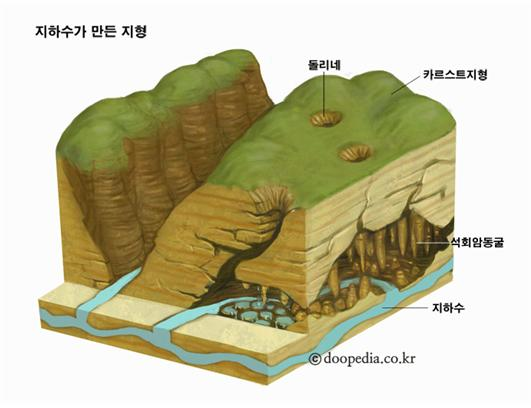
\includegraphics[width=0.9\textwidth]{./fig/doline_0001.jpg}
				\end{figure}
				
			
		
		\clearpage  \null \vskip 1em
		\subsection{민둥산 돌리네}
		

				강원도 정선군. 석회암 내 탄산칼슘이 빗물에 용해되어 지반이 침하된 카르스트 지형을 볼 수 있다. 민동산 일대에는 총 12개의 돌리네가 있다.

				석회암 지대의 갈라진 틈으로 이산화탄소를 포함한 빗물이 스며들면 석회암의 주성분인 탄산칼슘이 녹아서 깔때기 모양 또는 작은 양념절구 모양의 오목하게 패인 웅덩이를 형성한다. 
				크기는 지름 1m 내외에서 100m에 이르는 등 다양하나, 최근의 국제적인 정의(定義)에 따르면 그 와지 저면(底面)에서 경작할 수 있는 토양이 발달할 정도의 크기를 돌리네라고 하기로 하였다. 
				돌리네의 저면에는 테라로사(terra rossa)라고 불리는 토양이 발달된 곳이 많으며, 경작지로 이용되고 있다.

			또한 돌리네가 더욱 용식(溶蝕)되어 인접된 돌리네와 연결되어 좁고 긴 와지를 이루는 경우를 우발레(uvale)라고 한다. 
			아드리아해(海) 동안의 카르스트 지방, 일본의 야마구치현[山口縣] 아키요시다이[秋吉臺]가 세계적으로 알려졌으며, 한국의 충북 단양(丹陽) 일대에도 매포(梅浦)를 중심으로 하여 다수의 돌리네가 형성되어 있다. 

	

	

		\clearpage  \null \vskip 1em
		\subsection{석회암  라피에 lapie}

				기반암이 석회암인 지역에서 석회암이 용식되어 울퉁불퉁해진 후 토양층이 제거되면 석회암은 원추형의 암석기둥이나 능 모양의 소기복 지형을 이루게 되며, 이를 프랑스어로 라피에라고 한다. 
				독일어로는 카렌(karren)이라고 하며, 영국에서는 그리크(grike), 클린트(clint)라고 부른다. 

				토양층 위에 솟아 있는 모양이 공동묘지의 비석처럼 보이므로 ‘묘석지형’이라고도 불린다. 

				라피에는 피복식물 파괴지역이나 농업활동지역에서 잘 나타나며, 용식 기반면이 그대로 노출된 경우도 많다. 

				한편 라피에 군집을 라피아즈(lapiaz), 카렌펠트(karrenfeld)라고 한다. 
				과거 고생대의 해저환경에서 생성된 대석회암지대인 중국 화남지방의 구이린(桂林)의 라피에 군(群)은 세계적 관광명소가 되고 있으며, 우리나라의 강원도 삼척시 추암(楸岩) 해안에서도 소규모의 라피에가 관찰된다.


				\paragraph{1) 나출 라피에}




				\paragraph{2) 피복 라피에}




	
	\clearpage
%	----------------------------------------------------------------------------------------------------------------------- section
	\section{석회암 풍화토 terra rossa }



		\subsection{석회암 풍화토 terra rossa }


				석회암(탄산칼슘이 \%이상 함유) 이 용식을 받으면 탄산칼슘 성분은 제거되고 규산과 철, 알루미늄의 산화물 그리고 점토 광물 같은 비가용성 불순물은 제자리에 남게 된다. 
				이와 같은 불순물로 이루어진 석회암지대의 붉은 점토질 토양을 테라로사라고 한다. \\


				석회암은 고생대에 형성된 퇴적암을 말하며, 비가용성 물질이란 말은 물에 녹지 않는 성분이라고 보면 된다. 
				그래서 석회암 성분 중에서 다른 것들은 용탈(녹아서 밑으로 빠져버리는 것)되는데, 【 철 】, 【 알루미늄 】성분들은 녹지 않고 제자리에 남게 된다. 
				그러면 공기와 접하기 때문에 녹이 쓸어 붉은색을 갖는 것처럼 산화되어 적색을 갖게 된다. 
				그래서 테라고사는 색깔은 붉은 색이며 석회암지대에 나타나는 간대토양이라고 볼 수 있다. \\

				석회암은 특히 카르스트 지형이 형성되는 중요한 암석이기도 하다. 결론적으로 카르스트 지형이 많이 분포하는 석회암지대에 형성된 붉은 색의 간대토양을 테라로사로 한다.





% 	======================================================================================================================= chapter
	\clearpage
	\chapter{화산 쇄설암}
	\minitoc				% Creating an actual minitoc





	\clearpage
%	----------------------------------------------------------------------------------------------------------------------- section
	\section{화산 쇄설암}


			화산이 폭발할 때 방출되는 암편을 화산쇄설물(pyroclast)라고 하며, 화산쇄설물로 구성된 암석을 화산쇄설암이라고 한다. 
			
			화산쇄설물은 크기에 따라 화산암괴, 화산력, 화산회, 화산진 등으로 나뉜다. 
			
				화산암괴(火山巖塊, volcanic block, 64mm 이상)
				화산력(火山礫, lapilli, 2~64mm)
				화산회(火山灰, volcanic ash, 1/16~2mm)
				화산진(火山塵, volcanic dust, 1/16mm 이하)
			
			
			화산 분출물이 쌓여 굳으면서 이루어진 암석을 통틀어 이르는 말. 화산력, 각력암, 응회암 따위로 나눈다. [비슷한 말] 화성 쇄설암ㆍ화쇄암.
			
			\paragraph{1) 화산력 lapilli } \tab \tab
			
					화산력은 지름이 2~64mm에 해당하는 것으로 역질 응회암(Lapilli tuff)으로 고결된다. \\
					화산이 분출할 때에 터져 나오는 용암의 조각. 이미 굳어진 암석이 폭발하여 파괴된 것으로, 지름은 4~32mm이다.
					
					\begin{figure}[h]
					\centering
					\caption{화산력 lapilli }
					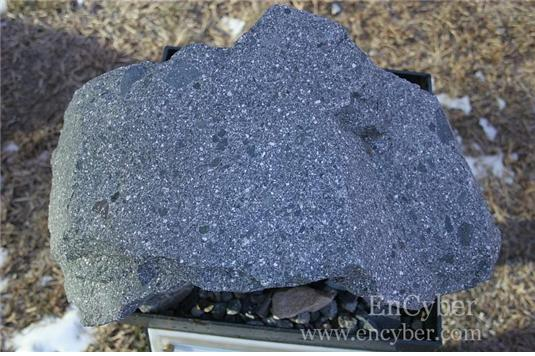
\includegraphics[width=0.8\textwidth]{./fig/lapilli_0001.jpg}
					\end{figure}
					
			
			\paragraph{2) 각력암 breccia } \tab \tab
			
					화산이 분출할 때에 터져 나오는 용암의 조각. 이미 굳어진 암석이 폭발하여 파괴된 것으로, 지름은 4~32mm이다.
					
					\begin{figure}[h]
					\centering
					\caption{각력암 breccia }
					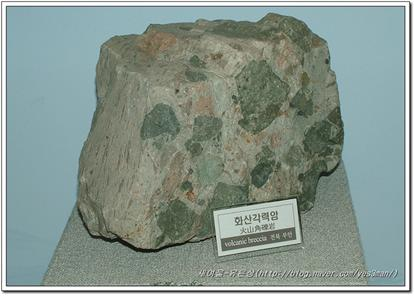
\includegraphics[width=0.8\textwidth]{./fig/breccia_0001.jpg}
					\end{figure}
					
					
			
			\paragraph{3) 응회암} \tab \tab
			
			화산이 분출할 때 나온 화산재 따위의 물질이 굳어져 만들어진 암석.



	\clearpage
%	----------------------------------------------------------------------------------------------------------------------- section
	\section{화산력}




	\clearpage
%	----------------------------------------------------------------------------------------------------------------------- section
	\section{각력암}
	
	
	
	
	\clearpage
%	----------------------------------------------------------------------------------------------------------------------- section
	\section{응회암}
	

		\paragraph{천성산 용연리 }
		이곳은 중생대 백악기 유문암과 안산암질암을 볼 수 있으며, 안산암질암이 유문암을 암맥상으로 관입하였다. 
		유문암은 암회색 또는 암갈회색의 반상조직을 보이며 반정은 사장석과 알칼리장석으로 구성되고 기질은 매우 치밀한 은미정질이다. 
		부분적으로 흰색의 암편이 함유되기도 하며, 이들 암편과 반정이 일정한 방향성을 보이는 유상구조로 되어 있다. 
		또 지표에서 굳어지면서 수평절리와 수직절리가 높은 밀도로 발달되어 심한 파쇄대처럼 보인다. 
		이 유문암을 관입한 암회색 또는 흑색의 안산암질암은 반정이 사장석으로 구성된 반상조직을 보이며 
		부분적으로는 각력질 안산암(brecciated andesite)이 산출되기도 한다. \\

		용연리 백악기 유문암과 안산암질 응회암 [Cretaceous rhyolite and andesitic tuff at Yongyeon-ri, Yangsan] (한국의 지질노두, 초판 2004., 개정판 2013., 한국지질자원연구원)








	\clearpage
%	----------------------------------------------------------------------------------------------------------------------- section
	\section{규질암 chert}


				이산화규소가 많이 들어 있는 암석.
				

	\clearpage
%	----------------------------------------------------------------------------------------------------------------------- section
	\section{규조암 diatomite  硅藻岩 }

	
				규질연니가 고화된 퇴적암으로 처트같은 치밀한 규산질 퇴적암.



			\paragraph{규조}
				평균 크기 50 내지 100 마이크로미터 크기의 규조류(diatome)라고 불리는 부유성 조류(藻類; algae) 껍데기로 이루어진 퇴적물의 집합체이다.

				이들 규조는 살아 생전에 물에서 실리카를 흡수해 세포벽을 만든다. 
				이러한 규조들의 퇴적물이 속성 작용을 받아 굳어져 퇴적암을 만들면 규조암(diatomite)라고도 하는데, 통상적으로 이것도 함께 광석의 의미로 규조토로 합쳐 부른다.



				규조는 diatom, 규조연니(토)는 diatomaceous ooze(earth)이다. 
				규조연니가 대부분인 암석을 규조암(diatomite)이라 하며, 이 암석이 단단하게 규질화된 것을 규조 처트라고 한다. 
				방산충 처트와 같이 유기질 퇴적암에 속한다. 
				
				북미의 지명 Tripoli에서 나온 tripolite도 같은 의미로 쓰이는 지역 암석명이다.  \\
				
				규조암은 규조의 껍데기로 구성된 규질 퇴적암이며 단백석은 규조암의 기본 구성광물이다. 
				육안으로 보면 이 암석은 우백색이고 부스러지기 쉬우며 미세한 공극을 갖는다. 
				규조암은 일종의 유기질 처트이다.

				해수의 수심 4,000~5,000m를 탄산염의 보상심도(compensation depth)라고 하는데 이보다 깊은 심해는 탄산염이 불포화상태이기 때문에 녹아 없어져 해저에 퇴적된 생물기원 연니에는 탄산염이 함유되지 않는다. 
				따라서 깊은 곳에는 규산염 연니, 낮은 곳에는 탄산염 및 규산염 연니가 발달된다.

			• 산출지 : 독일의 Celle, L. Saxony 부근의 Unterlüss













% 	======================================================================================================================= chapter
	\newpage
	\chapter{해식 이암 Sea Stack}


	% -------------------------------------- page -------------------
	%	\nomtcrule         		% removes rules = horizontal lines
	%	\nomtcpagenumbers  % remove page numbers from minitocs
%		\newpage
		\minitoc				% Creating an actual minitoc
	%	\doublespace





	\clearpage
%	----------------------------------------------------------------------------------------------------------------------- section
	\section{해식 이암 Sea Stack}



	\subsection{해식 이암}
	
	

				조석 간만의 차에 의해 해안가에 드러나는 기암 지형을 지형학 용어로는 시스택(Sea stack), 또는 해식이암(海蝕離岩)이라고 한다. \\
				
				시스택은 해풍에 오랫동안 침식을 받아 암석의 약한 부분은 침식되어 바다속으로 사라지고 강한 부분만 남은 것이다. 이러한 지형은 우리나라 해안 곳곳에 널리 발달해 있는데 특히 바다로 돌출한 암석 해안에 잘 나타난다. \\
				
				백령도의 두무진, 울릉도의 코끼리바위, 홍도의 독립문바위, 제부도의 매바위, 서귀포의 외돌개, 동해의 추암 등이 대표적인 예이다.





	\clearpage
%	----------------------------------------------------------------------------------------------------------------------- section
	\section{해식 이암 부산 오륙도}
	

	\subsection{	부산 오육도}
	

			부산에는 밀물 때와 썰물 때 암석의 수가 달라 보여 흥미를 끄는 시스택 ( sea stack )이 있다. 
			그것은 바로 부산의 상징이자 자랑거리인 오륙도(五六島)이다.  \\
			
			오륙도는 부산만의 북쪽 해안인 승두말에서 부산만을 향해 가지런히 뻗어 있는 5개의 시스택으로 이루어진 바위섬이다. 
			\textbf{우삭도} (32m), \textbf{수리섬} (33m), \textbf{송곳섬}(37m), \textbf{굴섬} (68m), \textbf{등대섬} (27m) 
			이렇게 옹이종기 모여 있는 5개의 섬이 밀물 때는 6개, 썰물 때는 5개로 보여 오륙도라는 이름이 붙었다. \\
			
			오륙도라고 불리게 된 이유는 5개의 섬 가운데 육지에서 가장 가까운 우삭도의 지형적 특징과 조차 때문이다. 
			\textbf{우삭도}를 자세히 살펴보면 섬 중간으로 나 있는 폭 1m, 높이 9m의 해식동에 의해 \textbf{방패섬}과 \textbf{솔섬}으로 분리되어 있다. 
			이들 섬은 물이 들면 해식대 위로 바닷물이 올라와 2개의 섬으로 완전히 분리되고, 물이 빠지면 해식동의 기저를 이루는 해식대가 해수면 위로 나타나 하나의 섬이 된다. 
			이렇게 때로는 5개의 섬으로, 때로는 6개의  섬으로 보이니 오륙도만큼 어울리는 이름도 없을 것이 \\
			
			
			
			그러나 1740년에 편찬된 《동래부지(東萊府誌)》〈산천(山川)〉조에 나타난 다음의 기록을 보면 ja 이음에 대한 해석이 나온다. 
			“절영도(지금의 영도) 동쪽에 있는 오륙도는 기이한 봉우리를 이루며 바다 가운데 나란히 섰는데 동쪽에서 보면 여섯 봉우리가 되고, 서쪽에서 보면 다섯봉우리가 되어 그리 이름했다”  \\
			
			이 기록으로 보아 예전에는 동과 서의 위치와 방향에 따라 한 섬이 보였다가 보이지 않았다가 하여 오륙도라고 불렀음을 알 수 있다. 
			어쨌든 1740년 이전부터 이미 오륙도라는 이름이 사용되고 있었던 것은 분명하다.
			



	\subsection{오륙도의 지질}
	

			오륙도가 위치한 부산만 북안 일대의 지질은 태종대의 해식 암벽에서 볼 수 있는 퇴적암과 거의 같은 시기인 약 1억년 전을 전후한 \textbf{ 중생대 } \textbf{ 백악기 }에 형성된 \textbf{ 퇴적암 }이다.
			\textbf{역암층}이 주를 이루며 그 사이에는 약 10 cm 두께의 \textbf{사암층}이 끼어 있다. 
			이러한 퇴적암은 부산만 북안에 위치한 승두말과 오륙도에 걸쳐 동일하게 나타난다. 
			이는 오륙도가 해식 작용을 받아 현재의 해식이암으로 분리되기 이전에는 승두말과 이어진 하나의 반도로서 바다로 돌출된 헤드랜드( head land ) 였음을 뜻한다. 
			그렇다면 오륙도는 어떤 과정을 거쳐 지금의 시스택이 된 것일까 ? \\
			
			오륙도의 섬들은 거의 수직에 가까운 80~85의 해식 절벽을 이루는데, 그 절벽면에는 많은 절리가 발달해 있다
			. 이런 절리면에는 파도에 의한 침식이 집중되어 암석이 깎여나간다. 
			과거 승두말에서 바다로 돌출한 반도 전역에 해식이 진행되었다고 볼 수 있다. 
			먼저 암석에 난 수직의 절리면을 따라 침식이 강하게 진해되어 암석의 일부분이 떨어져 나가면서 해식동이 여러 개 생겨났다. 
			이후 이것이 더욱 확대되어 5개의 시스택으로 분리되었다. 
			이와 동시에 수평의 역암층 사이에 끼인 사암층이 침식에 약해 보다 쉽게 분리, 제거되면서 여러 개의 파식대가 형성되었다. 
			이렇게 오륙도는 절리면을 따라 작용한 수직적 파식과 암석의 경연(硬軟)에 따른 수평적 파식 작용이 함께 만들어낸 것이라 할 수 있다. \\
			
			승두말과 오륙도가 하나의 반도로 연결되어 있던 시기는 해수면이 현재보다 6m 가량 높았던 12만 년 전이라고 한다. 
			그러므로 오륙도는 12만년 이라는 긴 시간동안 바다의 지속적인 침식을 받아 지금의 모습이 된 것이다. \\
			
			해식애의 기저에는 규모는 작지만 파식에 의해 형성된 해식동이 여러 개 나타난다. 
			그 중 가장 뚜렷한 모양은 \textbf{굴섬}과 \textbf{우삭도}에 나타나는데, 우삭도의 해식동은 폭이 1m  정도이고 굴섬의 해식동은 폭이 5m 에 달한다, 
			이 해식동 앞쪽으로 파식이 계속 이루어지고 있기 때문에 머지않아 오륙도는 8개 혹은 9개의 해식이암으로 변할 것이다. \\
			


	\subsection{오륙도의 파식대}
	

			오륙도는 \textbf{역암층}이 주를 이루는 퇴적암으로 그 사이에는 \textbf{사암층}이 끼어 있다. 
			모래는 자갈에 비하여 침식에 매우 약하기 때문에 사암층은 역암층보다 파도에 쉽게 씻겨나간다. 
			오륙도에는 이와 같은 지질 조건이 수평적으로 반영되어, 규모는 크지 않지만 여러 개의 파식대가 나타난다. \\
			 
			오륙도의 파식대는 모두 4개로 해발고도 27m, 17m, 9m, 0.5m 부근에 나타나는데 0.5m 파식대를 제외한 나머지 3단의 파식대에는 육상 식물이 자생하고 있다. 
			이 파식대들은 과거의 바다 환경에서 침식을 받은 후 융기한 것이다. 따라서 오륙에는 현재와 같은 해식 지형이 형성되기 이전에 적어도 세차례의 간헐적인 지반 상승이 있었던 것으로 보인다. \\
			
			과거의 해수면에서 침식을 받아 평탄해진 파식대가 어느 시기에 융기했는지에 대해서는 아직까지 유효한 자료가 없어 단정 짓기 어렵다. 
			이와 관련하여 고 오건환 교수는 27m 파식대는 오륙도가 육지의 승두말과 연결되었을 당시의 해수면에서 파도의 침식을 받아 형성된 것으로, 그 시기를 최종 간빙기 최성기였던 약12만 년 전으로 보았다. 
			그리고 9m 파식대는 최종 간빙기인 3만~2만 5,000년 전에 해수면이 일시 정체했던 시기에 형성된 것으로, 그 중간에 위치한 17 m 파식대는 27 m 파식대와 9 m 파식대의 중간시기인 약 5만~3만 5,000년 전에 형성된 것으로 보았다. 
			한편 최저위의 0.5m 파식대는 현재의 바다에 의해 형성된 현성(現成) 파식대로 육지와 가장 가까운 우삭도에서 넓게 나타난다. \\
			
			이를 통해 볼 때 지반 융기에 의한 단구성 파식대가 여러 개 나타나는 오륙도는 과거의 지반 융기 운동과 해수면 변화 등의 영향을 받은 화석 지형임과 동시에 현재도 계속적인 변화를 겪고 있는 현성 지형이기도 한다.




% ------------------------------------------------------------------------------
% End document
% ------------------------------------------------------------------------------

\end{document}


		%		\tabulinesep=0.6ex
				\begin{tabu} to 1.0\textwidth { X[l, 1.0] X[l, 2.0] X[l, 2.0] X[l, 2.0] }
				\tabucline[0.2ex]{-}		
				품명				&규격		&단가	&비고\\
				\tabucline[0.1ex]{-}		
				결명자			&				&		&\\
				\tabucline[0.1ex]{-}		
				\end{tabu} 



				\paragraph{필수 재료}
				\begin{itemize}[topsep=0.0em, parsep=0.0em, itemsep=0em, leftmargin=12.0em, labelwidth=3em, labelsep=3em] 
				\item [두부] 		1/2 모
				\item [녹말가루] 	3
				\item [무] 		1/2 토막
				\item [쪽파] 		1 대
				\end{itemize}

				\begin{itemize}[topsep=0.0em, parsep=0.0em, itemsep=0em, leftmargin=12.0em, labelwidth=3em, labelsep=3em] 
				\item 
				\end{itemize}

				\begin{figure}[h]
				\centering
				\caption{화산 각력암}
				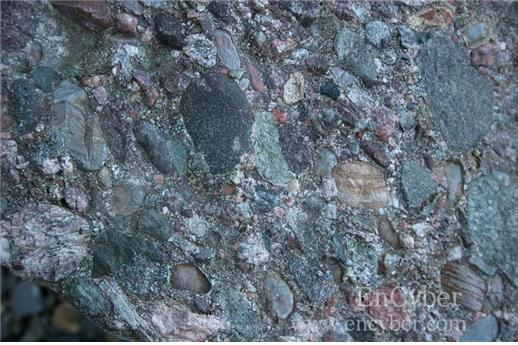
\includegraphics[width=0.8\textwidth]{./fig/SedimentaryRock_0002.jpg}
				\end{figure}


% 	======================================================================================================================= chapter
	\newpage
	\chapter{베거너}


	% -------------------------------------- page -------------------
	%	\nomtcrule         		% removes rules = horizontal lines
	%	\nomtcpagenumbers  % remove page numbers from minitocs
%		\newpage
		\minitoc				% Creating an actual minitoc
	%	\doublespace


	\clearpage
%	----------------------------------------------------------------------------------------------------------------------- section
	\section{베거너}




